% xelatex
\documentclass[12pt]{article}

\usepackage{polyglossia}
\usepackage{pgfplots}
\setmainlanguage{czech}

\usepackage{graphicx, xevlna, minted} %graphics files inclusion
\usepackage{url}
\usepackage{hyperref}
\usepackage[style=iso-numeric]{biblatex}

\usepackage{hyperref}
\hypersetup{
    colorlinks=true,
    linkcolor=blue,
    filecolor=magenta,      
    urlcolor=cyan,
}

\title{
\includegraphics[width=8cm]{cvut-logo-bw.pdf}\\\vspace{2cm}NI-KOP \\ Exaktní a heuristická řešení konstruktivního problému batohu}
\author{\small Petr Pondělík} %doplňte své jméno, jméno vedoucího a svůj studijní obor
\date{\small Fakulta informačních technologií Českého vysokého učení technického v Praze, \\ Thákurova 9, 160 00 Praha 6 \\ \url{pondepe1@fit.cvut.cz}} %doplňte svůj email

\addbibresource{ref.bib}

\begin{document}

\maketitle              

\newpage

\section{Specifikace úlohy}

(plná verze dostupná na: \href{https://moodle-vyuka.cvut.cz/mod/assign/view.php?id=89697}{Zadání Moodle})

Jsou dány sady instancí (známe jejich optimální řešení) konstruktivní verze optimalizačního 0/1 problému batohu, a to:

\begin{itemize}
    \item sada NK náhodně vygenerovaných instancí \\ pro \(n=4, 10, 15, 20, 22, 25, 27, 30, 32, 35, 37, 40\)
    \item sady ZKC a ZKW ve stejném rozsahu n, o jejichž generování není nic známo
\end{itemize}

Naprogramujte řešení konstruktivní verze problému batohu:

\begin{itemize}
\item hrubou silou
\item metodou větví a hranic
\item metodou dynamického programování (dekompozice podle kapacity nebo podle cen),
\item jednoduchou greedy heuristikou
\item modifikací této heuristiky (redux)
\item FPTAS algoritmem
\end{itemize}

Na zkušebních instancích experimentálně vyhodnoťte závislost výpočetního času a u všech heuristických algoritmů také relativní chyby (průměrné i maximální)  na velikosti instance. Proveďte testování na všech sadách instancí (NK, ZKC, ZKW). Jednotlivé sady instancí vyhodnocujte zvlášť. Pozorujte rozdíly mezi nimi.

\newpage

\section{Varianty řešení}

V základu problému batohu máme zadány následující proměnné: 

\begin{itemize}
    \item celé číslo n (počet věcí)
    \item celé číslo M (kapacita batohu) 
    \item konečná množina \( V=\{v_1,v_2,…,v_n\} \) (hmotnosti věcí) 
    \item konečná množina \( C=\{c_1,c_2,…,c_n\} \) (ceny věcí)
\end{itemize}

V konstruktivní verzi optimalizačního 0/1 problému batohu hledáme množinu \( X=\{x_1,x_2,…,x_n\} \) (konfigurace) kde každé \( x_i \in \{0,1\} \) tak, aby platila nerovnost \( \sum_{i=1}^{n} x_i v_i \leq M \) (omezení) a suma \( \sum_{i=1}^{n} x_i c_i \) byla maximální (optimalizační kritérium).

\subsection{BruteForce}

\subsubsection{Rozbor řešení}

Pro nalezení optimálního řešení vyhodnotíme všechny konfigurace problému. V případně nalezení lepšího řešení aktualizujeme stávající optimum. Vzhledem k definici množiny X, představující množinu konfigurací, je složitost této varianty řešení $2^n$.

\subsubsection{Postup řešení}

Strom konfigurací rekurentně procházíme celý, během průchodu jsou zaznamenávány volby $x_i$ a v případě nalezení lepšího řešení je aktualizováno aktuální optimum. Aktualizace optimálního řešení probíhá pouze v případě, že konfigurace splňuje podmínku $ \sum_{i=1}^{n} x_i c_i > C_{opt} $ či obě podmínky $ \sum_{i=1}^{n} x_i c_i = C_{opt} $ a $\sum_{i=1}^{n} x_i v_i < M_{opt}$, kde $C_{opt}$, resp. $M_{opt}$ jsou cena, resp. hmotnost aktuálního optimálního řešení.

\newpage

\subsubsection{Kostra algoritmu}

\begin{listing}[ht]
    \begin{minted}[fontsize=\footnotesize]{python}
# Globálně dostupná proměnná opt (defaulně nulová cena, nekonečná hmotnost)

# První krok rekurze 
vyhodnotInstanci():
    zpracujStav(uroven = 1, prvni predmet nepridan, konfigurace = [])
    zpracujStav(uroven = 1, prvni predmet pridan, konfigurace = []) 
    return optimalni reseni
 
zpracujStav(uroven, stav, konfigurace): 
    konfigurace.append(stav.x)
    if uroven >= n: 
        updatujOptimum(stav, konfigurace) 
        return 
    zpracujStav(uroven++, predmet nepridan, konfigurace.add(True))
    konfigurace.pop()
    zpracujStav(uroven++, predmet pridan, konfigurace.add(False))
    konfigurace.pop()

updatujOptimum(stav, konfigurace): 
    if (
        stav.hmotnost < M and (
            stav.cena > opt.cena or ( stav.cena == opt.cena and stav.hmotnost < opt.hmotnost)
        )
    ):
        updatuj optimalni reseni aktualnim stavem a konfiguraci
    \end{minted}
\end{listing}

\subsection{Branch\&Bound}

\subsubsection{Rozbor řešení}

Řešení problému je možné optimalizovat prořezáváním stavového prostoru. Pro dosažení rozumné optimalizace je nutné prořezávat prostor jak shora (překročení kapacity batohu), tak zdola (stávající řešení nemůže být lepší než nejlepší dosud nalezené). Asymptotická složitost řešení je stále $O(2^n)$.

\subsubsection{Postup řešení}

Ořezávání shora je implementováno testováním podmínky na aktuální hmotnost v každém rekurentním volání. Ořezávání zdola je implementováno testováním, zda v dané větvi rekurze potenciálně lze dosáhnout lepšího řešení, než je aktuální optimální řešení. Testování spočívá v přičtení sumy cen všech zbývajících předmětů k ceně aktuálního stavu a její srovnání s cenou aktuálně nejlepšího řešení.

\subsubsection{Kostra algoritmu}
\begin{listing}[ht]
    \begin{minted}[fontsize=\footnotesize]{python}
# Globálně dostupná proměnná opt (defaulně nulová cena, nekonečná hmotnost)
vyhodnotInstanci():
    zpracujStav(uroven = 1, prvni predmet nepridan, konfigurace = [])
    zpracujStav(uroven = 1, prvni predmet pridan, konfigurace = []) 
    return optimalni reseni
 
zpracujStav(uroven, stav, konfigurace): 
    konfigurace.append(stav.x)
    if stav.hmotnost > M: return
    if not potencialneLepsi(uroven, stav): return
    if uroven >= n: 
        updatujOptimum(stav, konfigurace) 
        return 
    zpracujStav(uroven++, predmet nepridan, konfigurace.add(True))
    konfigurace.pop()
    zpracujStav(uroven++, predmet pridan, konfigurace.add(False))
    konfigurace.pop()

potencialneLepsi(uroven, stav):
    ziskej zbyvajici predmety dle urovne
    pCena = stav.cena + suma cen zbyvajicich predmetu
    pHmotnost = stav.hmotnost + suma cen zbyvajicich predmetu
    return pCena > opt.cena or (pCena == opt.cena and pHmotnost < opt.hmotnost)

updatujOptimum(stav, konfigurace): 
    if (
        stav.hmotnost < M and (
            stav.cena > opt.cena or (stav.cena == opt.cena and stav.hmotnost < opt.hmotnost)
        )
    ):
        updatuj optimalni reseni aktualnim stavem a konfiguraci
    \end{minted}
\end{listing}

\newpage

\subsection{Greedy heuristika}

\subsubsection{Rozbor řešení}

Greedy heuristika staví na plnění batohu předměty v sestupném pořadí dle poměru \(\frac{cena}{hmotnost}\). Nevýhodou je, že její chyba není shora omezena.

\subsubsection{Postup řešení}

Pro instanci o vel. $n$ je definována konfigurace $\{x_1=0,...,x_n=0\}$. Předměty jsou seřazeny dle poměru \(\frac{cena}{hmotnost}\). Následně jsou iterovány a dokud řešení po zahrnutí předmětu nepřekročí kapacitu $M$, je předmět přidán do řešení. V případě přidání i-tého předmětu je v konfiguraci nastavena hodnota $x_i=1$ a cena řešení je inkrementována o jeho hmotnost.

\subsubsection{Kostra algoritmu}

\begin{listing}[ht]
    \begin{minted}[fontsize=\footnotesize]{python}
solution # Globální proměnná (defaulně nulová cena a hmotnost)
X = [0, ..., 0] # Pole o velikosti instance
for item in items:
    if solution.weight + item.weight <= M:
        solution.cost += item.cost
        solution.weight += item.weight
        X[item.inx] = 1
    \end{minted}
\end{listing}

\subsection{Greedy heuristika (redux)}

\subsubsection{Rozbor řešení}

Cena řešení nalezeného pomocí základní greedy heuristiky je porovnána s cenou řešení, které se skládá z jediné věci, a to nejcennější takové, že se do batohu vejde. Lepší z této dvojice je pak finálním řešením. Chyba heuristiky je shora omezena na 50 \%.

\subsubsection{Postup řešení}

Stejný jako v případě základní heuristiky. Navíc je vyhledána druhá varianta řešení (viz rozbor) a výsledkem je lepší z nalezených řešení.

\subsubsection{Kostra algoritmu}

\begin{listing}[ht]
    \begin{minted}[fontsize=\footnotesize]{python}
solution, solutionRedux # Globální proměnné (defaulně nulová cena a hmotnost)
X = [0, ..., 0], XRedux = [0, ..., 0] # Pole o velikosti instance
findBasicSolution() # viz předchozí heuristika
reduxSolutionInx = -1
for item in items:
    if item.weight <= self.M and item.cost > solutionRedux.cost:
        solutionRedux.weight = item.weight
        solutionRedux.cost = item.cost
        reduxSolutionInx = item.inx
XRedux[reduxSolutionInx] = 1
return betterSolution(solution, solutionRedux)
    \end{minted}
\end{listing}

\subsection{Dynamické programování}

\subsubsection{Rozbor řešení}

Dynamické programování (DP) využívá dekompozici instance problému. Řešení podproblémů vzniklých dekompozicí jsou ukládána do paměti a znovupoužita v případě potřeby řešit již známý podproblém. DP tedy převádí časovou složitost na složitost paměťovou.

Pro řešení problému batohu pomocí DP lze využít dekompozici dle váhy či ceny. V případě dekompozice dle ceny pak hledáme řešení inverzního problému batohu. Tedy pro daný počet předmětů n a cenu C hledáme konfiguraci \( X=\{x_1,x_2,…,x_n\} \) takovou, aby \( \sum_{i=1}^{n} x_ic_i = C \) (omezení) a suma \( \sum_{i=1}^{n} x_iw_i \) byla minimální (optimalizační kritérium).

Velikost potřebné paměti je \(n \sum_{i=1}^{n}c_i\). Každý prvek lze spočítat v konstantním čase. Nechť \(C_M = max\{c_1, c_2, ..., c_n\}\). Pak \(\sum_{i=1}^{n}c_i \leq n C_M\). Asymptotická složitost této varianty je tedy \( O(n^2 C_M) \). Parametr $C_M$ nezávisí na velikosti instance, tudíž se jedná o pseudopolynomiální algoritmus.

\subsubsection{Postup řešení}

Využita je dekompozice dle ceny. DP je vyřešeno iterativně. Alokována je tabulka \textbf{memory} hmotností (hodnoty $\infty$) o velikosti $(n+1)(C_{sum}+1)$, kde $C_{sum}=\sum_{i=1}^{n}c_{i}$. Z optimalizačního důvodu jsou ceny předmětů s hmotností přesahující M nastaveny na 0 (nižší $C_{sum}$). Definujeme $memory[0][0]=0$. Následně jsou řešeny postupně rostoucí podproblémy o $n^{'}$ prvcích z množiny $\{1,...,n\}$ plnění batohu tak, aby $\sum_{i=1}^{n^{'}} x_ic_i = C$ (omezení) a suma $\sum_{i=1}^{n^{'}} x_iw_i$ byla minimální. Opakující se podproblémy nejsou opakovaně počítány, ale je využíváno již vyřešených podproblémů. Minimální váha, pomocí které lze dosáhnout ceny $c$ pro instanci o $i+1$ prvních předmětech, je získána vztahem $memory[c][i+1] = min(memory[c][i], memory[c-c_{i+1}][i] + w_{i})$. Tedy zkoumáme, odkud jsme na aktuální pole tabulky mohli přistoupit v případě, že nový předmět nepřidáme ($memory[c][i]$), či přidáme ($memory[c-c_{i+1}][i] + w_{i}$) a vybíráme hodnotu s nižší hmotností.

Výslednou cenu $C_{res}$ nalezneme jako maximální řádkový index $c$ prvku posledního sloupce tabulky, jehož váha je $\leq M$. Konstrukce konfigurace řešení získáme pomocí backtrackingu z pozice ceny $C_{res}$. Vycházíme ze souřadnic optimálního řešení a postupně zmenšujeme řešený problém odebíráním předmětů. Pokud se při zmenšení problému nezmění minimální hmotnost (porovnání $memory[c][i] = memory[c][i-1]$), předmět nepatří do konfigurace řešení.

\newpage

\subsubsection{Kostra algoritmu}

\begin{listing}[ht]
    \begin{minted}[fontsize=\footnotesize]{python}
# Globální proměnné
n, M, C, W, cSum, solution
memory = [[inf for i in {0, ..., n+1}] for j in {0, ..., cSum+1)]
memory[0][0] = 0
for i in {1, ..., n+1}:
    for cost in C:
        memory[cost][i+1] = min(memory[cost][i], memory[cost - C[i+1]][i] + W[i])

findSolution(memory):
    return memory[c,n], kde memory[c,n] <= M a c je maximalni

findSolutionConf(memory, cost):
    conf = [0 for i in {0, ..., n}]
    actualCost, actualItem = cost, n
    for i in {1, n + 1}:
        originItem, originCost = actualItem-1, actualCost
        originWeight = self.memory[actualCost][originItem]
        actualWeight = self.memory[actualCost][actualItem]
        if actualWeight != originWeight:
            originCost = actualCost - C[n-i]
            conf[n-i] = 1
            actualCost, actualItem = originCost, originItem
    return conf

solution.cost = findSolution(memory)
solution.configuration = findSolutionConf(memory, solution.cost)

return solution

    \end{minted}
\end{listing}

\newpage

\subsection{FPTAS algoritmus}

\subsubsection{Rozbor řešení}

Tento aproximativní algoritmus staví nad exaktním pseudopolynomiálním algoritmem pro řešení problému se složitostí $O(n^2 C_M)$, v našem případě se jedná o řešení problému batohu pomocí DP za využití dekompozice dle ceny.

Algoritmu je zadána požadovaná maximální relativní chyba $\epsilon$. Na základě $\epsilon$ je určena konstanta $k = \frac{\epsilon C_M}{n}$ sloužící pro redukci součtu cen, a tedy pro zmenšení paměťového prostoru.
Redukované ceny jsou získány vztahem $c_i^{'}~=~\lfloor\frac{c_i}{k}\rfloor$ pro $\forall i \in \{1, ..., n\}$.

Finální řešení je založeno na řešení instance $\{n, M, c_1^{'}, ..., c_n^{'}, w_1, ...,w_n\}$ získaném pomocí DP s dekompozicí dle ceny.

\subsubsection{Postup řešení}

Nejprve z důvodu optimalizace nastavíme nulovou cenu předmětům, jejichž hmotnost překračuje M, počet takto zredukovaných cen označíme $n_{reduced}$.

Vytvoříme zjednodušený model problému na základě zadané maximální relativní chyby $\epsilon$. Tedy získáme konstantu $k=\frac{\epsilon C_{M}}{n-n_{reduced}}$ ($k$ neovlivní předměty, jejichž cena byla redukována na 0). Následně získáme ceny $c_i^{'}$ dle postupu z rozboru.

Pomocí DP získáme konfiguraci ${x_1, ..., x_n}$ řešení zjednodušené instance $\{n, M, c_1^{'}, ..., c_n^{'}, w_1, ...,w_n\}$. Cenu řešení získáme jako $\sum_{i=1}^{n}x_ic_i$.

\newpage

\subsubsection{Kostra algoritmu}

\begin{listing}[ht]
    \begin{minted}[fontsize=\footnotesize]{python}
solution, eps, n, C, maxC W, nReduced # Globální proměnné

k = (eps * maxC)/(n - nReduced)
reducedC = [int(c/k) for c in C]
sumC = sum(reducedC)
memory = [[inf for i in {0, ..., n+1}] for j in {0, ..., sumC+1)]
memory[0][0] = 0

# DP nad zjednodušeným modelem
configuration = solveInstanceByDP(memory, reducedC, sumC)
solution.configuration = configuration
solution.cost = sum([configuration[i] * C[i] for i in {0, ..., n-1}])

return solution

    \end{minted}
\end{listing}

\newpage

\section{Naměřené výsledky}

\subsection{Specifikace platformy}

Procesor: Intel Core i5-10210U, 1.6 GHz (TurboBoost 4.2 GHz) \\
Operační systém: Kubuntu 20.04.1 LTS \\
Programovací jazyk: Python 3.8

\subsection{Sada NK}

\subsubsection{Závislost CPU času na velikosti instance}

Naměřené hodnoty reprezentují průměrný a maximální CPU čas potřebný k vyřešení jedné instance problém v milisekundách. Naměřené údaje jsou k dispozici v tabulce \ref{tab:nk_cpu_times}. Závislosti jsou vizualizovány v grafech \ref{fig:nk_cpu_time_avg}, \ref{fig:nk_cpu_time_avg_without_brute_force}, \ref{fig:nk_cpu_time_max} a \ref{fig:nk_cpu_time_max_without_brute_force}.

\begin{table}
    \begin{center} 
         \begin{tabular}{|c | c | c | c| c | c | c | c | c|} 
         \hline
         n & BF & BF max & B\&B & B\&B max & DP & DP max & Redux & Redux max \\ [0.1ex] 
         \hline\hline
        4 & 0,007 & 2 & 0,001 & 0,001 & 8,179 & 20 & 0,001 & 1 \\
        \hline
        10 & 4,573 & 5 & 0,401 & 2 & 55,309 & 100 & 0,001 & 1 \\
        \hline
        15 & 128,107 & 170 & 2,999 & 19 & 128,352 & 214 & 0,001 & 1 \\
        \hline
        20 & 4241,569 & 5075 & 23,533 & 287 & 269,604 & 439 & 0,001 & 0,001 \\
        \hline
        22 & 16682,322 & 18015 & 66,750 & 1032 & 329,721 & 505 & 0,001 & 1 \\
        \hline
        \end{tabular}
        \caption{CPU časy dle velikosti instance (sada NK)}
        \label{tab:nk_cpu_times}
    \end{center}
\end{table}

\begin{figure}[ht]\centering
    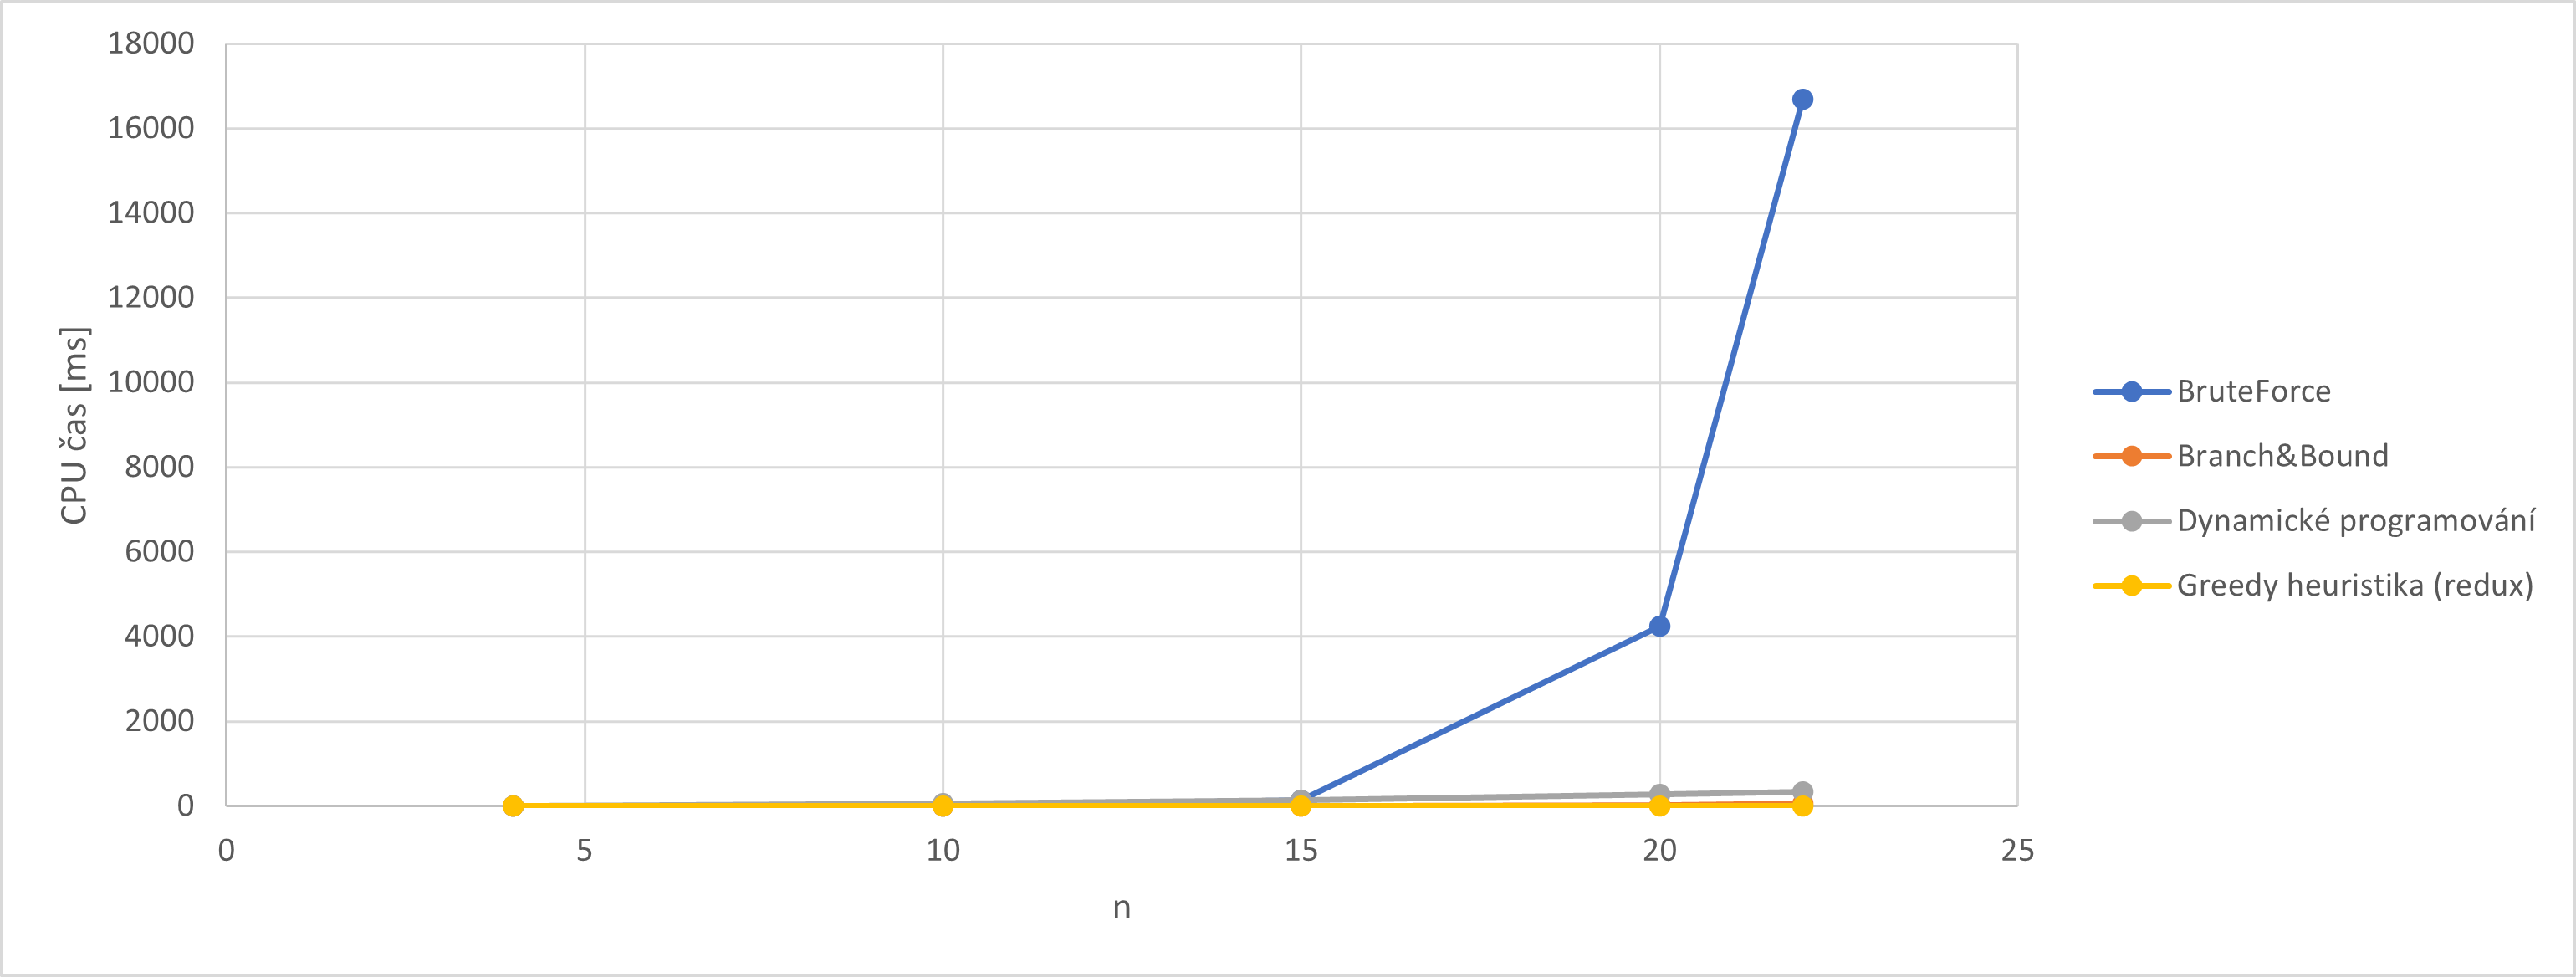
\includegraphics[width=1\textwidth, keepaspectratio]{graphs/NK/times/nk_cpu_time_avg.png}
    \caption{Závislost průměrného CPU času na n (sada NK)}
    \label{fig:nk_cpu_time_avg}
\end{figure}

\begin{figure}[ht]\centering
    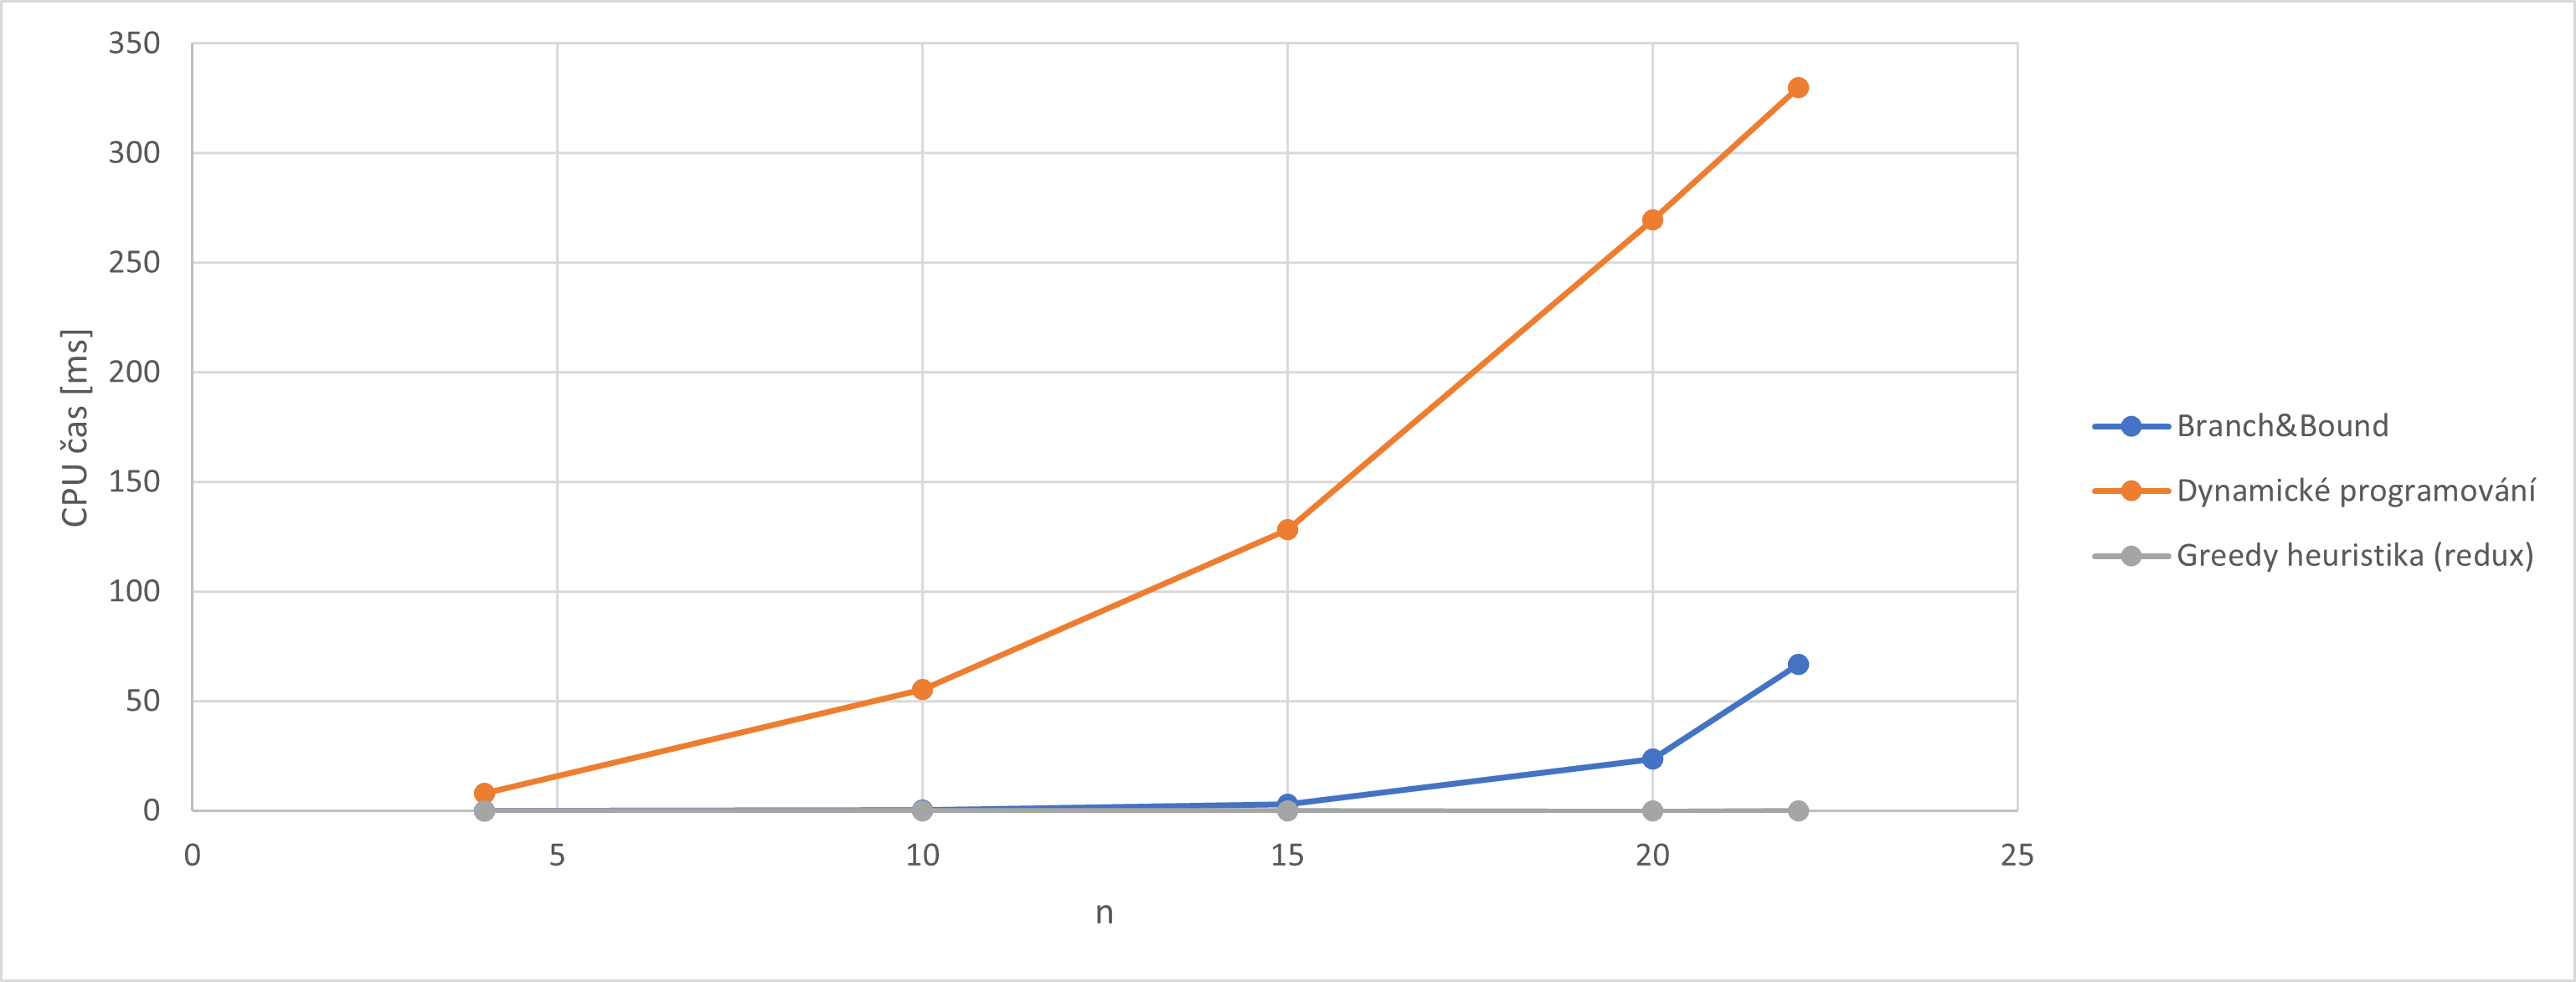
\includegraphics[width=1\textwidth, keepaspectratio]{graphs/NK/times/nk_cpu_time_avg_without_brute_force.png}
    \caption{Závislost průměrného CPU času (bez BruteForce) na n (sada NK)}
    \label{fig:nk_cpu_time_avg_without_brute_force}
\end{figure}

\begin{figure}[ht]\centering
    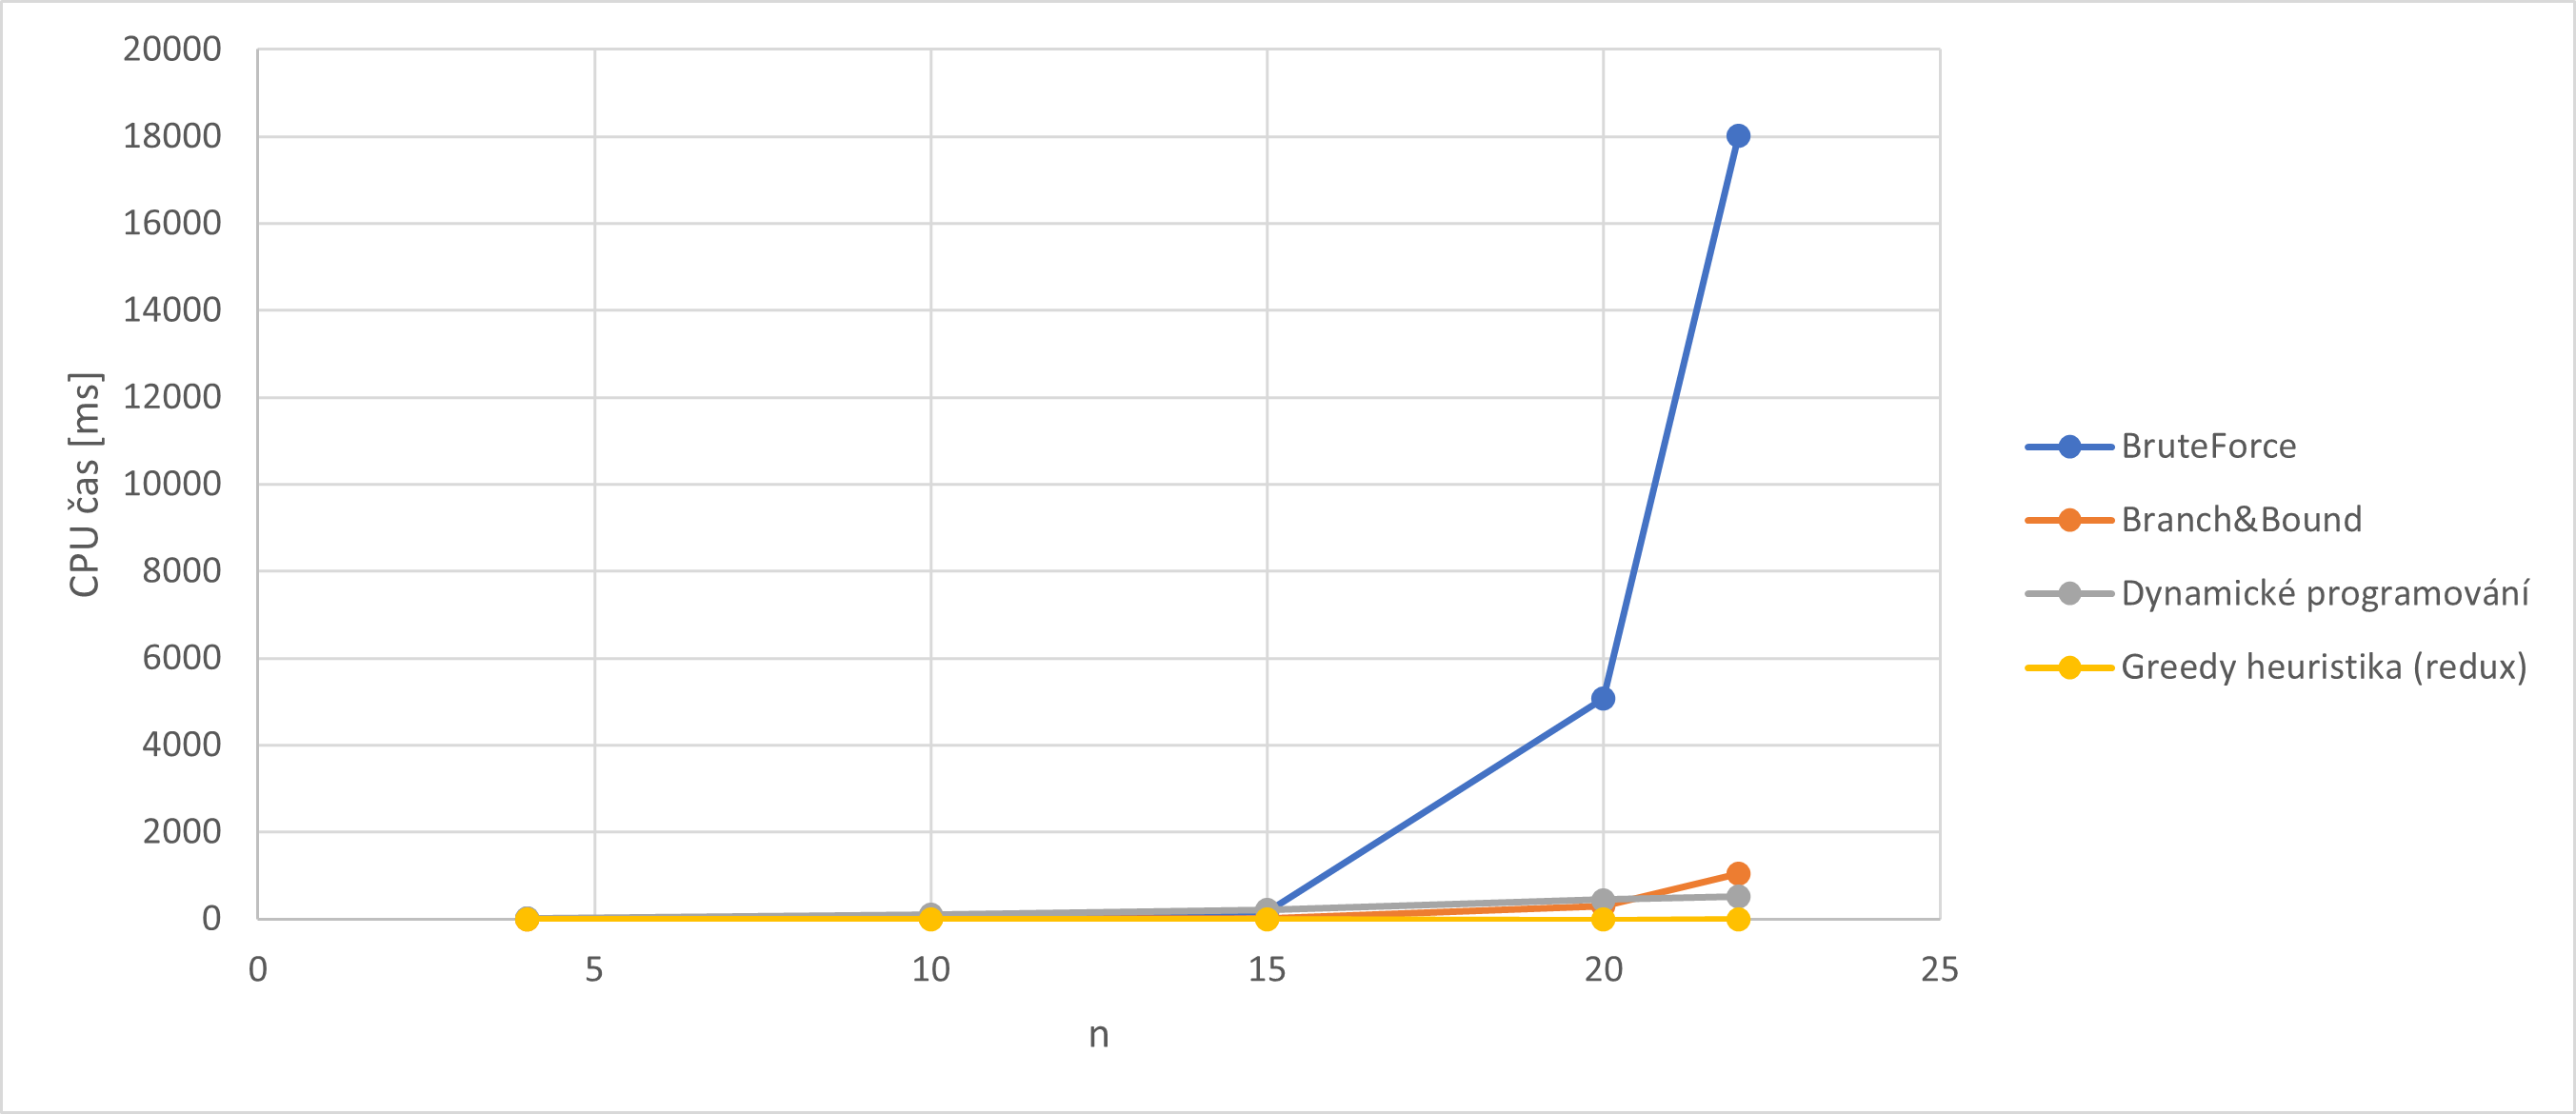
\includegraphics[width=1\textwidth, keepaspectratio]{graphs/NK/times/nk_cpu_time_max.png}
    \caption{Závislost maximálního CPU času na n (sada NK)}
    \label{fig:nk_cpu_time_max}
\end{figure}

\begin{figure}[ht]\centering
    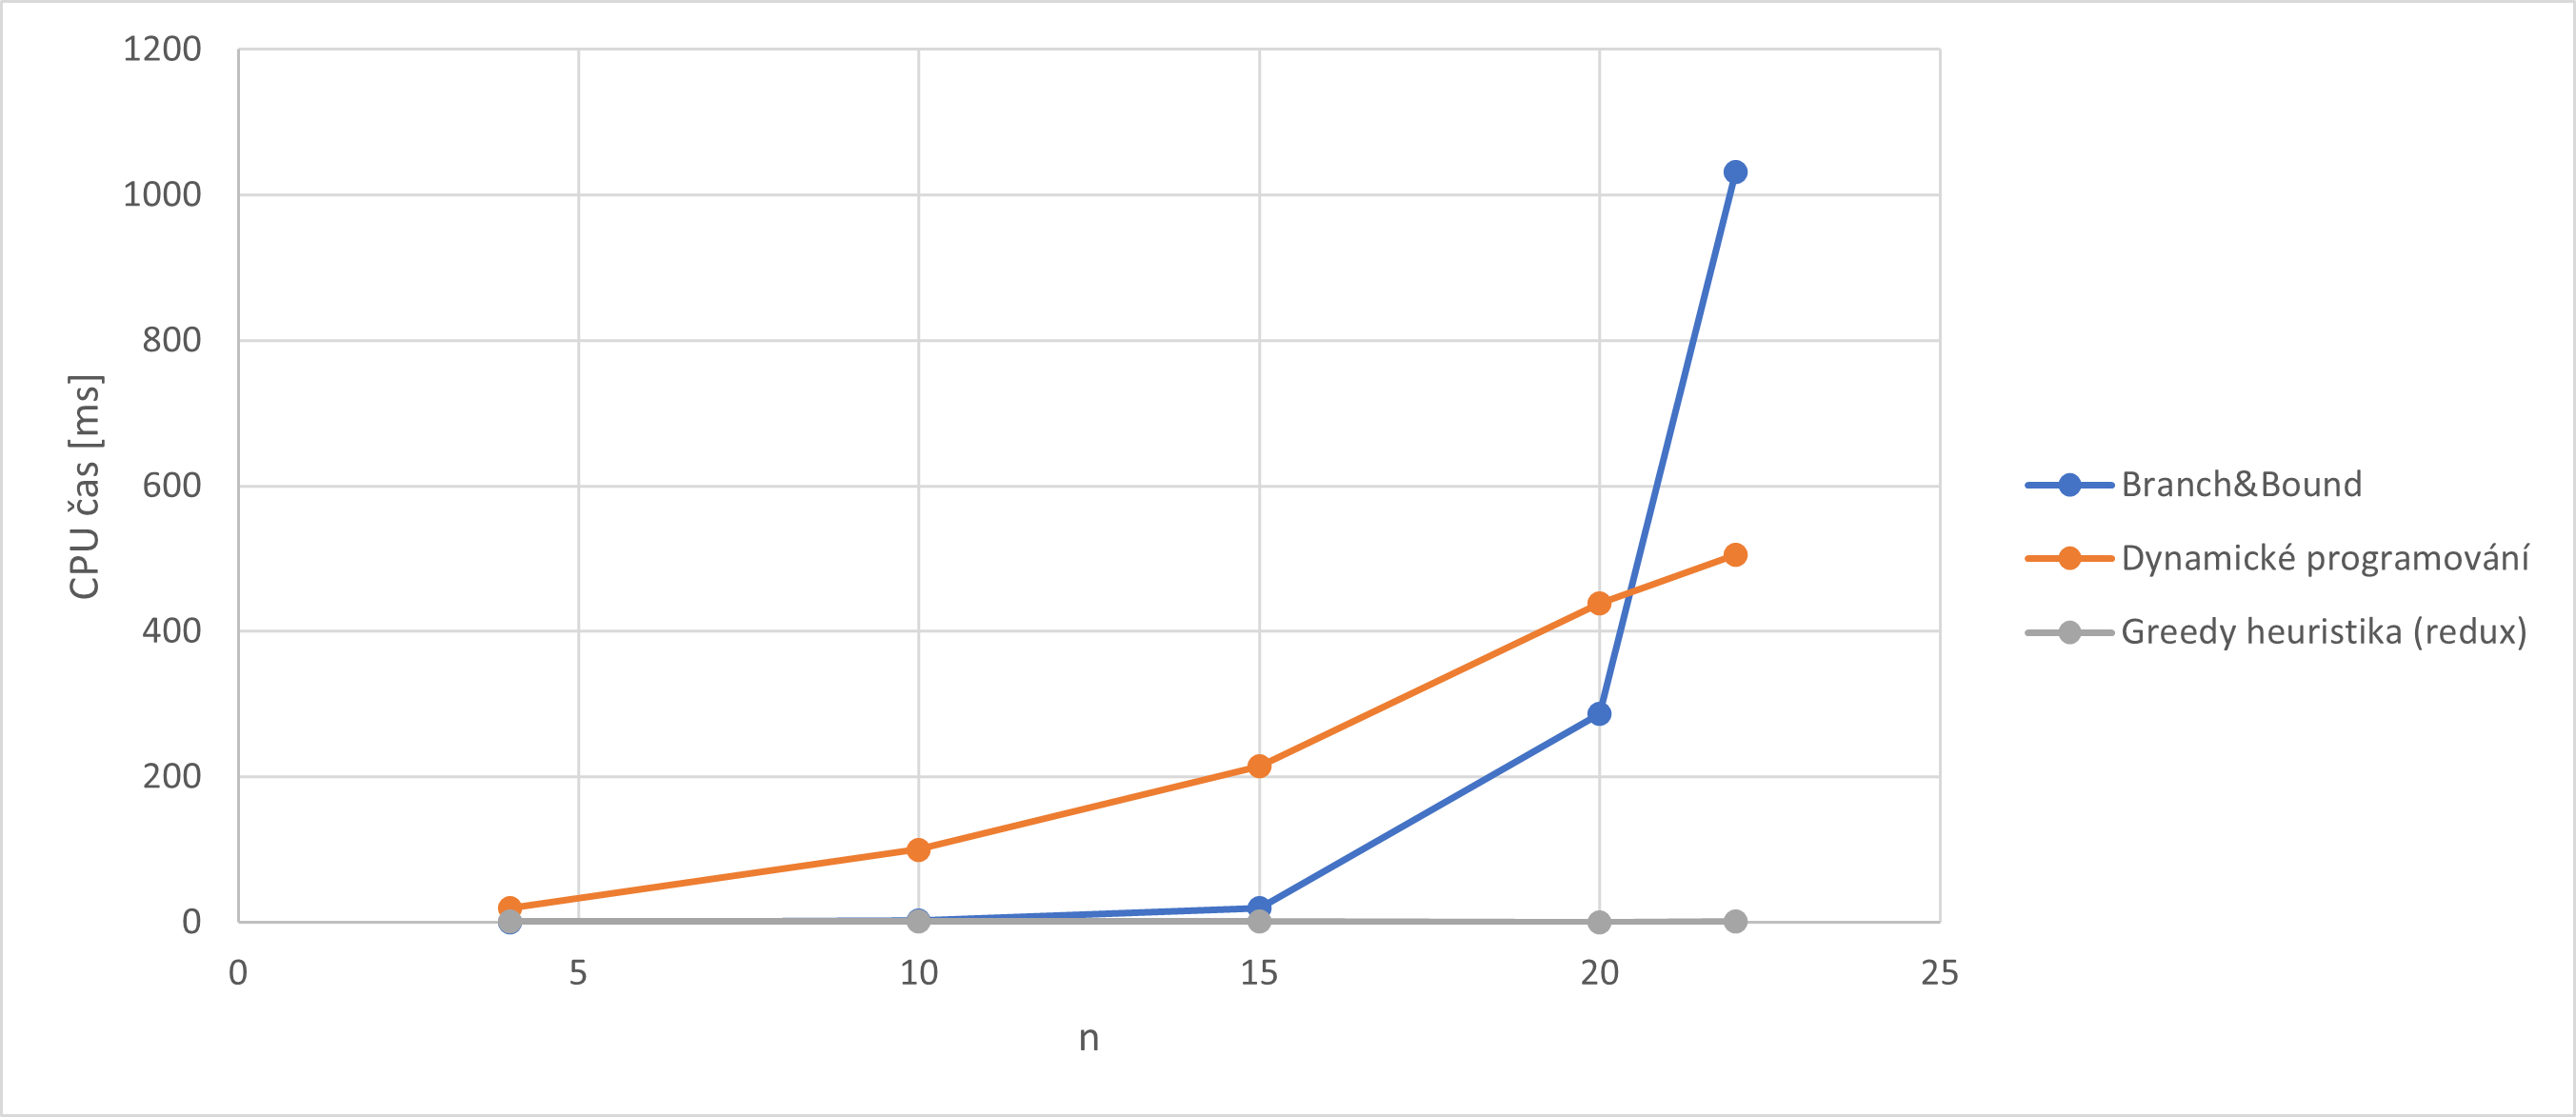
\includegraphics[width=1\textwidth, keepaspectratio]{graphs/NK/times/nk_cpu_time_max_without_brute_force.png}
    \caption{Závislost maximálního CPU času (bez BruteForce) na n (sada NK)}
    \label{fig:nk_cpu_time_max_without_brute_force}
\end{figure}

\subsubsection{Relativní chyby greedy heuristik}

Relativní chyba obou heuristik pro instanci problému $I$ byla získána vztahem $err_I = 1 - \frac{APR(I)}{OPT(I)}$, kde $APR(I)$ reprezentuje cenu řešení instance $I$ získaného heuristikou a $OPT(I)$ cenu optimálního řešení instance $I$. Naměřené údaje jsou k dispozici v tabulce \ref{tab:nk_greedy_error}. Závislosti jsou vizualizovány v grafech \ref{fig:nk_greedy_avg} a \ref{fig:nk_greedy_max}.

\begin{table}
    \begin{center}
         \begin{tabular}{|c | c | c | c | c|} 
         \hline
         n & Greedy & Greedy max & Greedy redux & Greedy redux max \\ [0.1ex] 
         \hline\hline
        4 & 1,453 & 35,919 & 1,219 & 35,919 \\
        \hline
        10 & 1,304 & 53,145 & 1,044 & 16,421 \\
        \hline
        15 & 0,968 & 23,683 & 0,926 & 23,683 \\
        \hline
        20 & 0,860 & 43,005 & 0,774 & 13,556 \\
        \hline
        22 & 0,779 & 40,385 & 0,663 & 13,181 \\
        \hline
        \end{tabular}
        \caption{Relativní chyby greedy heuristik (sada NK)} \label{tab:nk_greedy_error}
    \end{center}
\end{table}

\begin{figure}[ht]\centering
    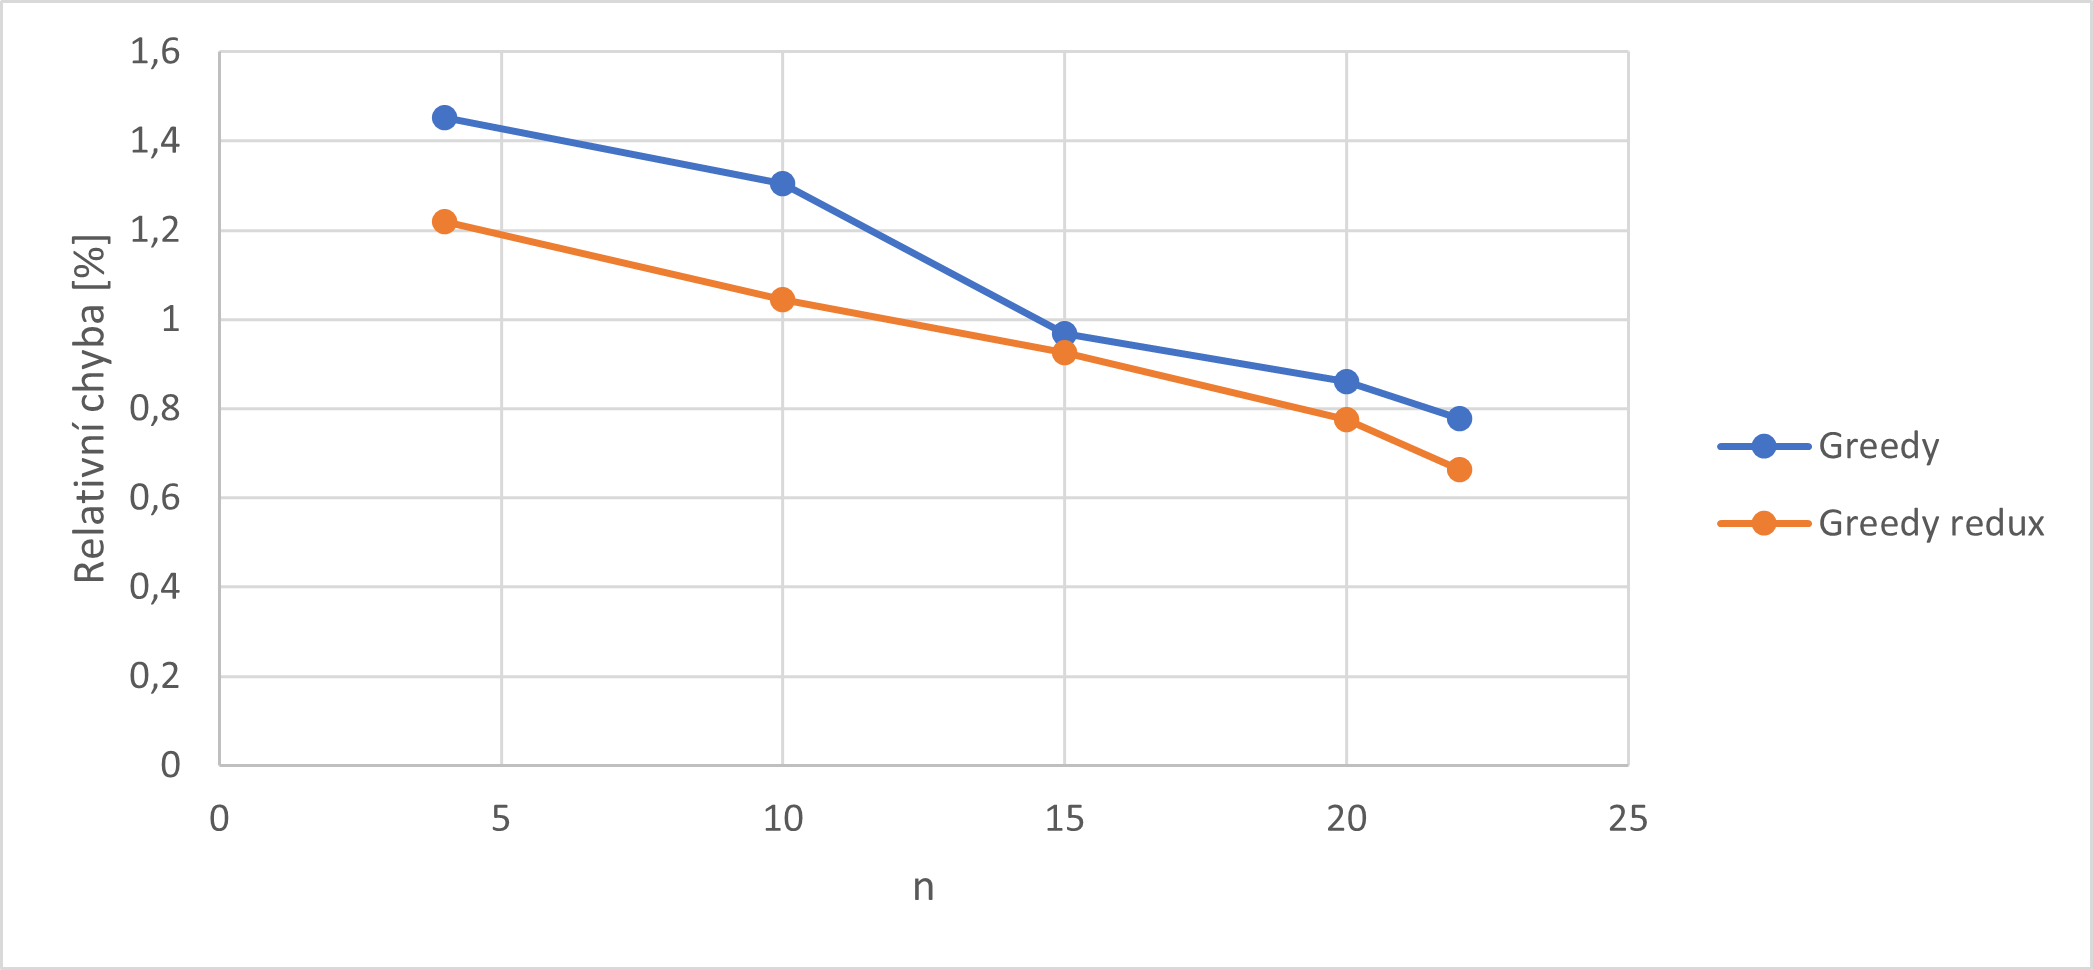
\includegraphics[width=1\textwidth, keepaspectratio]{graphs/NK/heuristics/nk_greedy_avg.png}
    \caption{Průměrná relativní chyba heuristik (sada NK)}
    \label{fig:nk_greedy_avg}
\end{figure}

\begin{figure}[ht]\centering
    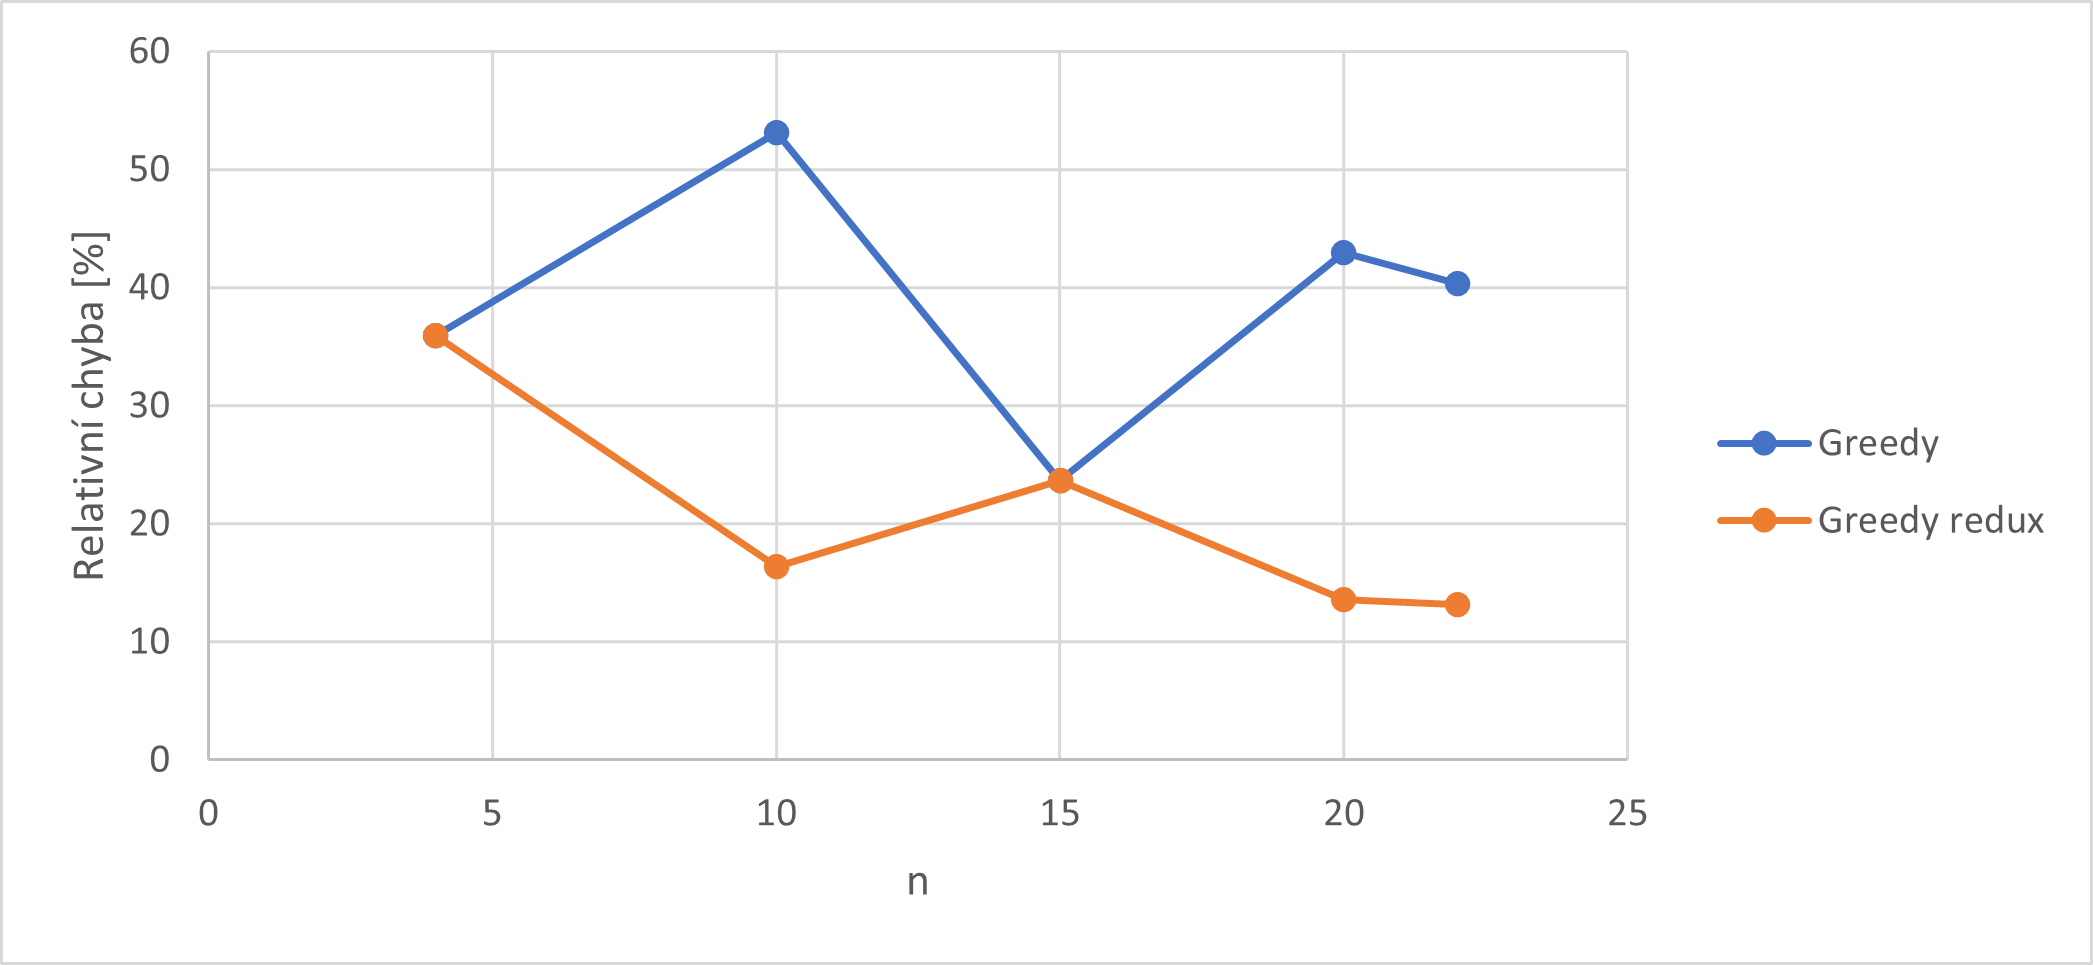
\includegraphics[width=1\textwidth, keepaspectratio]{graphs/NK/heuristics/nk_greedy_max.png}
    \caption{Maximální relativní chyba heuristik (sada NK)}
    \label{fig:nk_greedy_max}
\end{figure}

\subsubsection{CPU čas a chyby algoritmu FPTAS}

Naměřené hodnoty CPU času reprezentují průměrný a maximální CPU čas potřebný k vyřešení jedné instance problému v milisekundách. Pro účely měření byly zvoleny tři různé hodnoty n, pro něž byla pozorována závislost CPU času na $\epsilon$. Naměřené údaje jsou k dispozici v tabulce \ref{tab:nk_fptas_eps_times}. Závislosti CPU času jsou vizualizovány v grafech \ref{fig:nk_fptas_eps_time_avg} a \ref{fig:nk_fptas_eps_time_max}.

Hodnoty reálné maximální chyby $err_{real}$, resp. předpokládané maximální chyby $err_{upper}$ pro sadu instancí o velikosti $n$ s požadovanou maximální relativní chybou $\epsilon$ byly získány vztahem $err_{real} = max \forall I \{|OPT(I) - APR(I)|\}$, resp. $err_{upper} = \epsilon.OPT(I_{inx})$, kde $inx$ představuje id instance s maximální reálnou chybou.
Naměřené údaje jsou k dispozici v tabulce \ref{tab:nk_fptas_eps_error}. Závislosti reálné chyby FPTAS algoritmu jsou vizualizovány v grafu \ref{fig:nk_fptas_eps_error}. Srovnání reálné a maximální předpokládané chyby algoritmu FPTAS je k dispozici v grafu~\ref{fig:nk_fptas_eps_error_comparison}.

\begin{table}
    \begin{center}
         \begin{tabular}{|c | c | c | c | c | c | c|} 
         \hline
         $\epsilon$ & n=15 & n=15 (max) & n=20 & n=20 (max) & n=22 & n=22 (max) \\ [0.1ex] 
         \hline\hline
        0,1 & 8,215 & 15 & 19,615 & 29 & 25,740 & 41 \\
        \hline
        0,2 & 4,168 & 7 & 9,931 & 16 & 12,901 & 21 \\
        \hline
        0,3 & 2,805 & 5 & 6,656 & 12 & 8,629 & 14 \\
        \hline
        0,4 & 2,106 & 4 & 4,995 & 8 & 6,515 & 14 \\
        \hline
        0,5 & 1,763 & 3 & 3,985 & 7 & 5,594 & 15 \\
        \hline
        0,6 & 1,436 & 3 & 3,315 & 7 & 4,591 & 8 \\
        \hline
        0,7 & 1,085 & 2 & 2,851 & 6 & 3,921 & 7 \\
        \hline
        0,8 & 0,951 & 2 & 2,498 & 5 & 3,437 & 6 \\
        \hline
        0,9 & 0,925 & 2 & 2,146 & 4 & 3,071 & 6 \\
        \hline
        \end{tabular}
        \caption{CPU časy algoritmus FPTAS v závilosti na $\epsilon$ (sada NK)} \label{tab:nk_fptas_eps_times}
    \end{center}
\end{table}

\begin{figure}[ht]\centering
    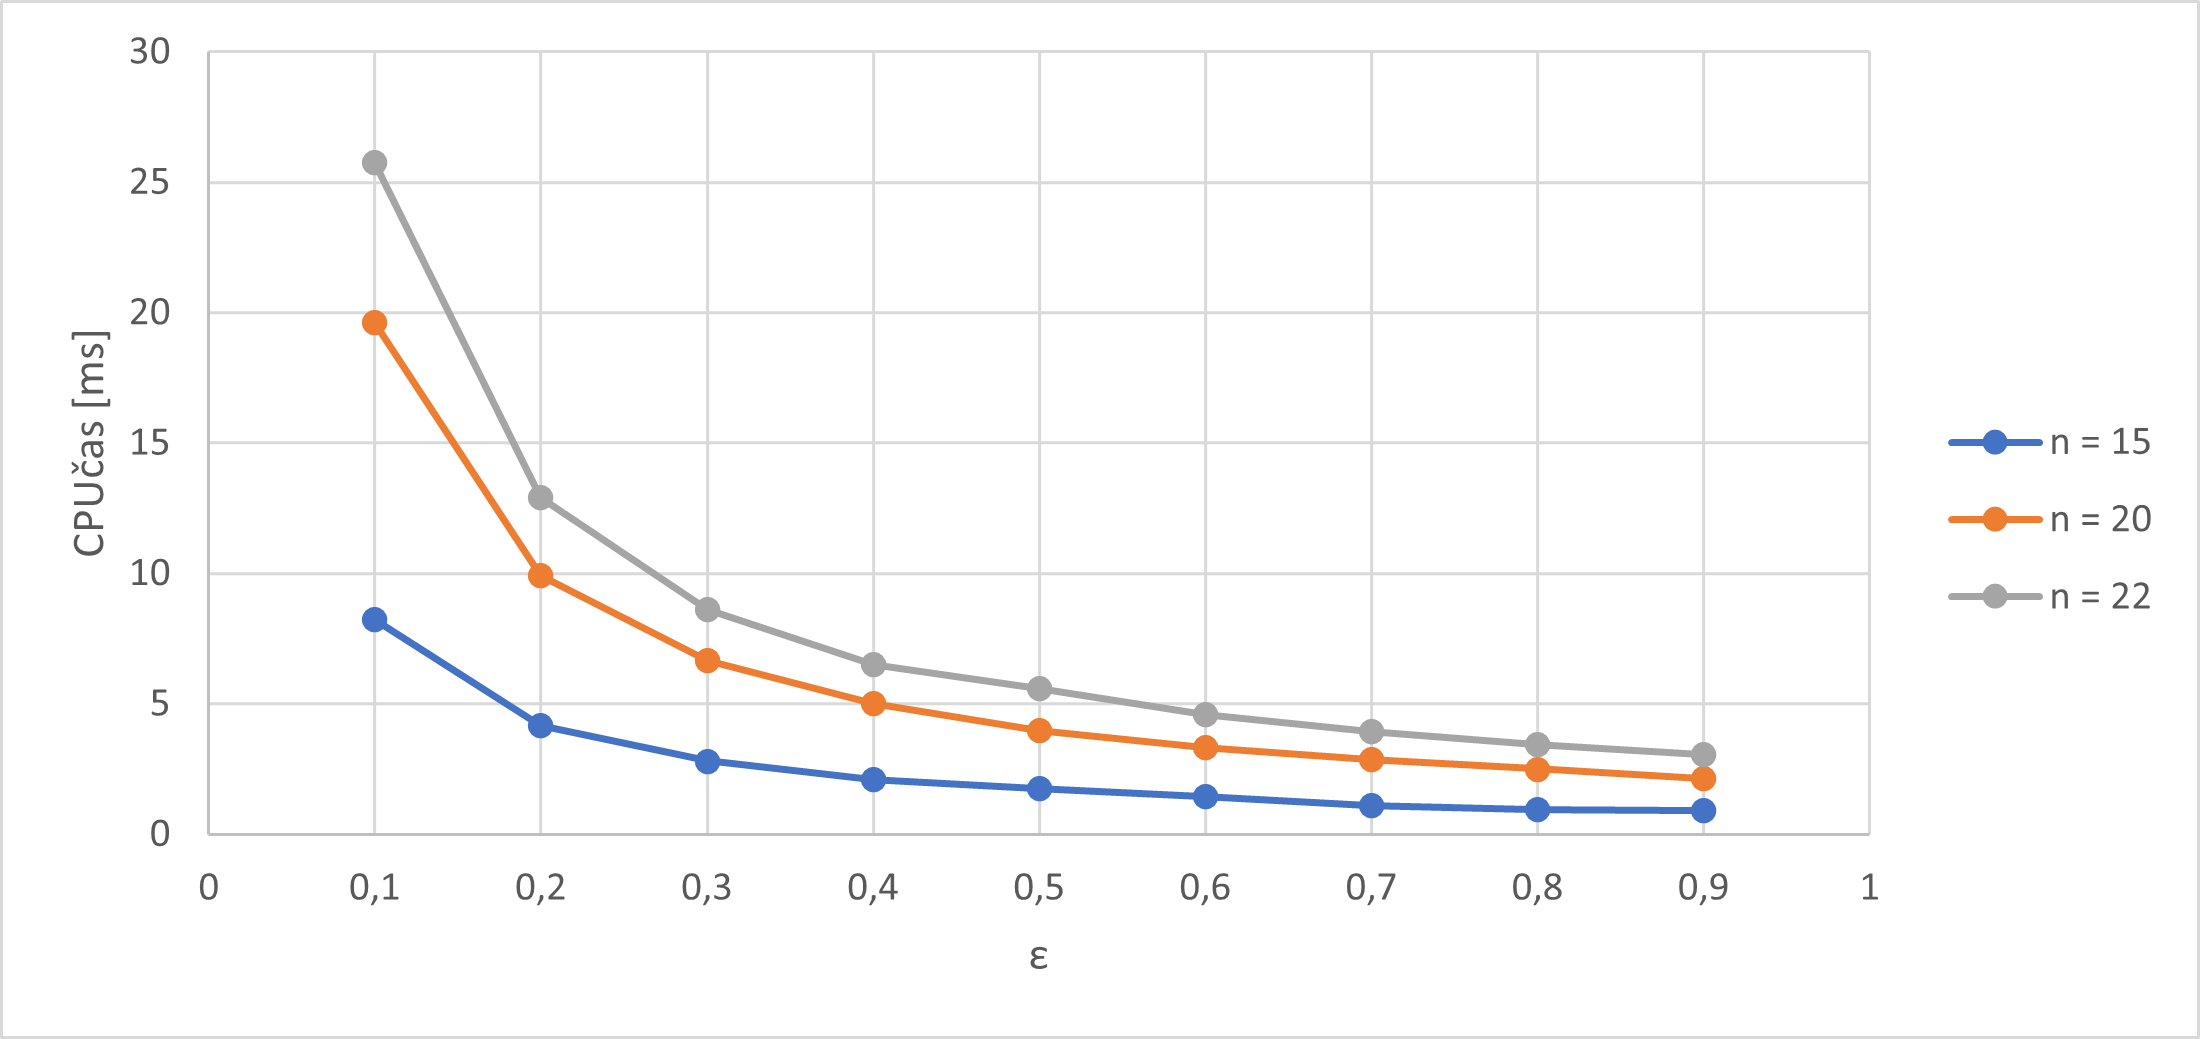
\includegraphics[width=1\textwidth, keepaspectratio]{graphs/NK/fptas/nk_fptas_eps_time_avg.png}
    \caption{Závislost průměrného CPU času FPTAS na $\epsilon$ (sada NK)}
    \label{fig:nk_fptas_eps_time_avg}
\end{figure}

\begin{figure}[ht]\centering
    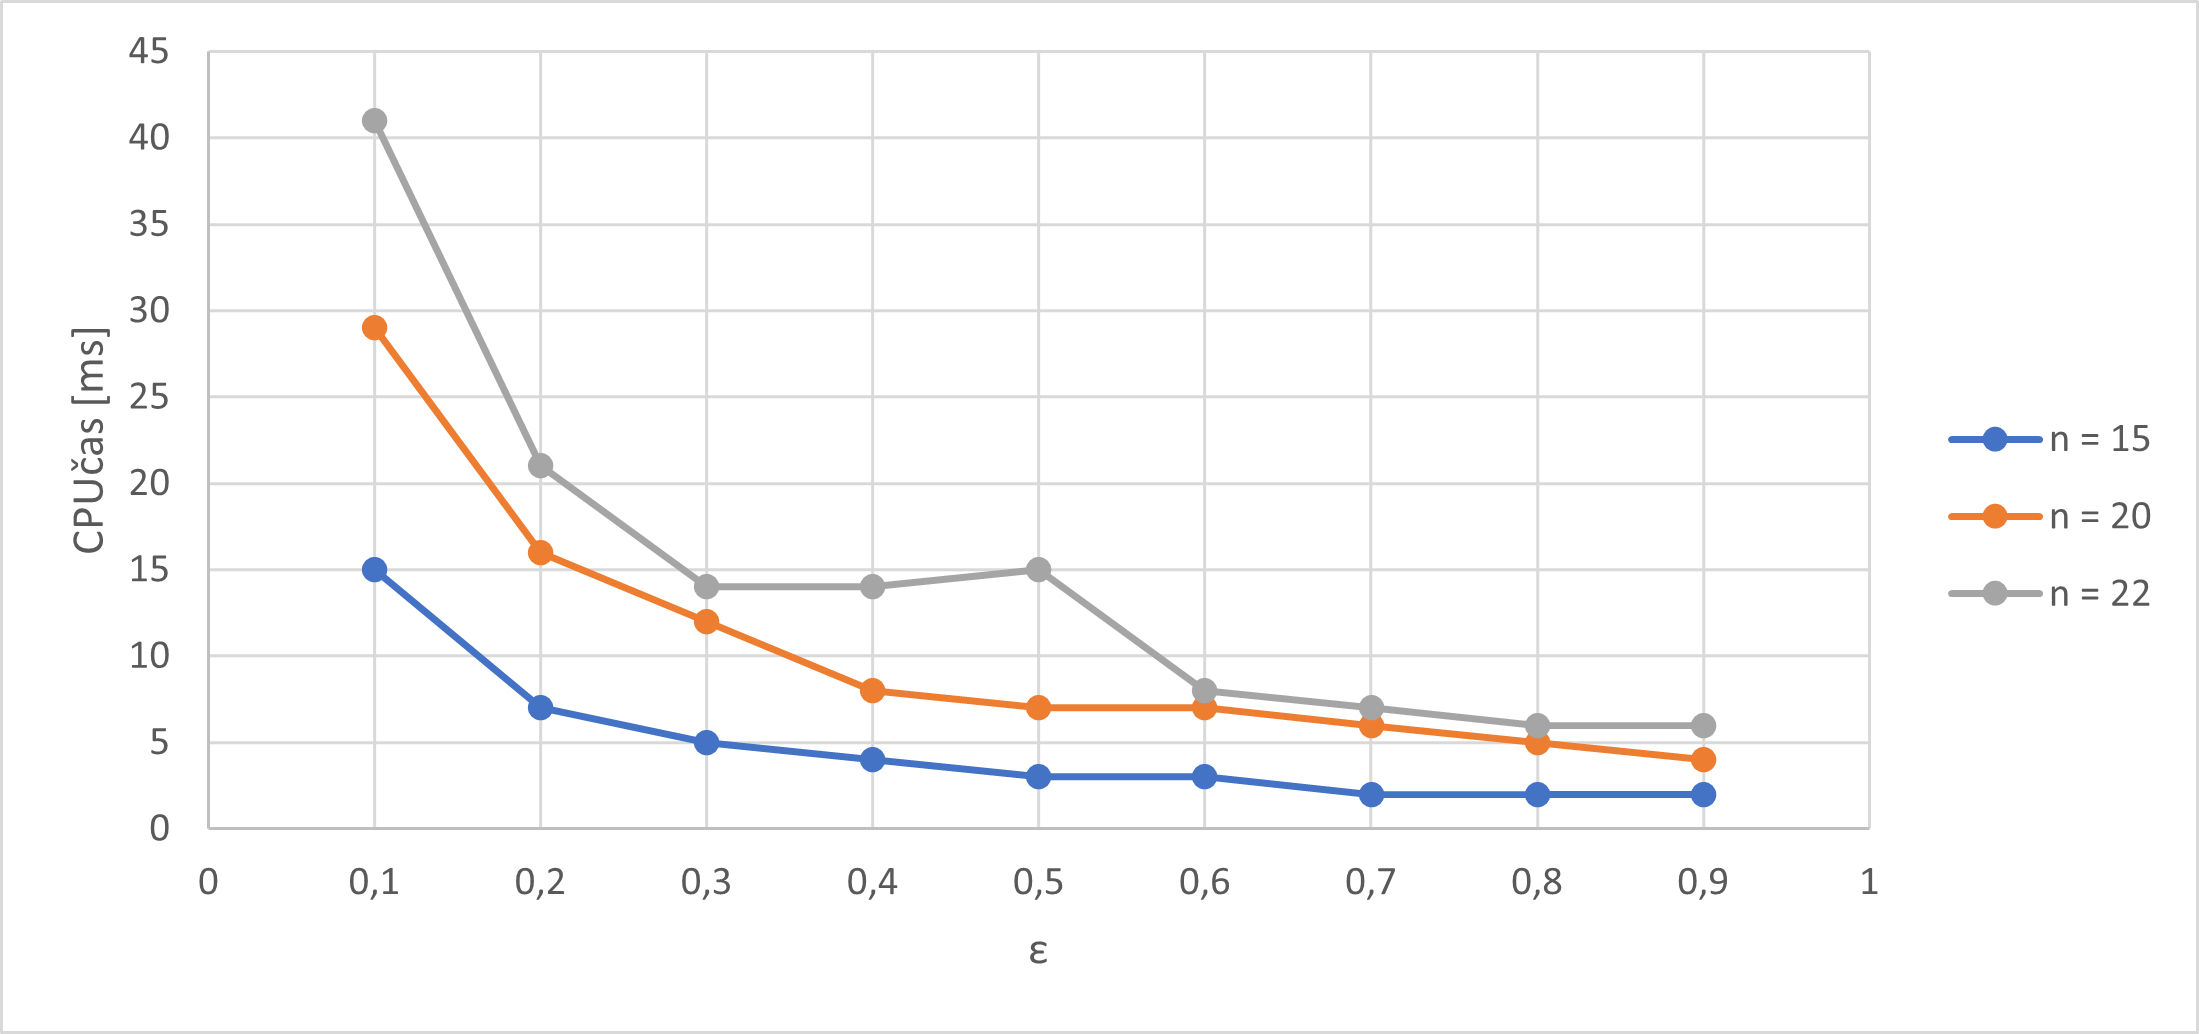
\includegraphics[width=1\textwidth, keepaspectratio]{graphs/NK/fptas/nk_fptas_eps_time_max.png}
    \caption{Závislost maximálního CPU času FPTAS na $\epsilon$ (sada NK)}
    \label{fig:nk_fptas_eps_time_max}
\end{figure}

\begin{table}
    \begin{center}
         \begin{tabular}{|c | c | c | c | c | c | c|} 
         \hline
         $\epsilon$ & n=15 & n=15 (předpoklad) & n=20 & n=20 (předpoklad) & n=22 & n=22 (předpoklad) \\ [0.1ex] 
         \hline\hline
        0,1 & 16 & 1051,700 & 10 & 515,200 & 17 & 658 \\
        \hline
        0,2 & 31 & 2711,200 & 22 & 2538,800 & 30 & 6154,800 \\
        \hline
        0,3 & 55 & 3256,200 & 153 & 1138,800 & 33 & 6969,900 \\
        \hline
        0,4 & 281 & 1734,800 & 153 & 1518,400 & 59 & 5471,200 \\
        \hline
        0,5 & 339 & 2573,500 & 149 & 1898 & 179 & 2024,500 \\
        \hline
        0,6 & 339 & 3088,200 & 153 & 2277,600 & 169 & 2128,800 \\
        \hline
        0,7 & 339 & 3602,900 & 249 & 3975,300 & 179 & 2834,300 \\
        \hline
        0,8 & 281 & 3469,600 & 153 & 3036,800 & 275 & 3239,200 \\
        \hline
        0,9 & 339 & 4632,300 & 249 & 5111,100 & 275 & 3644,100 \\
        \hline
        \end{tabular}
        \caption{Maximální reálné a předpokládané chyby algoritmu FPTAS v závislosti na $\epsilon$ (sada NK)} \label{tab:nk_fptas_eps_error}
    \end{center}
\end{table}

\begin{figure}[ht]\centering
    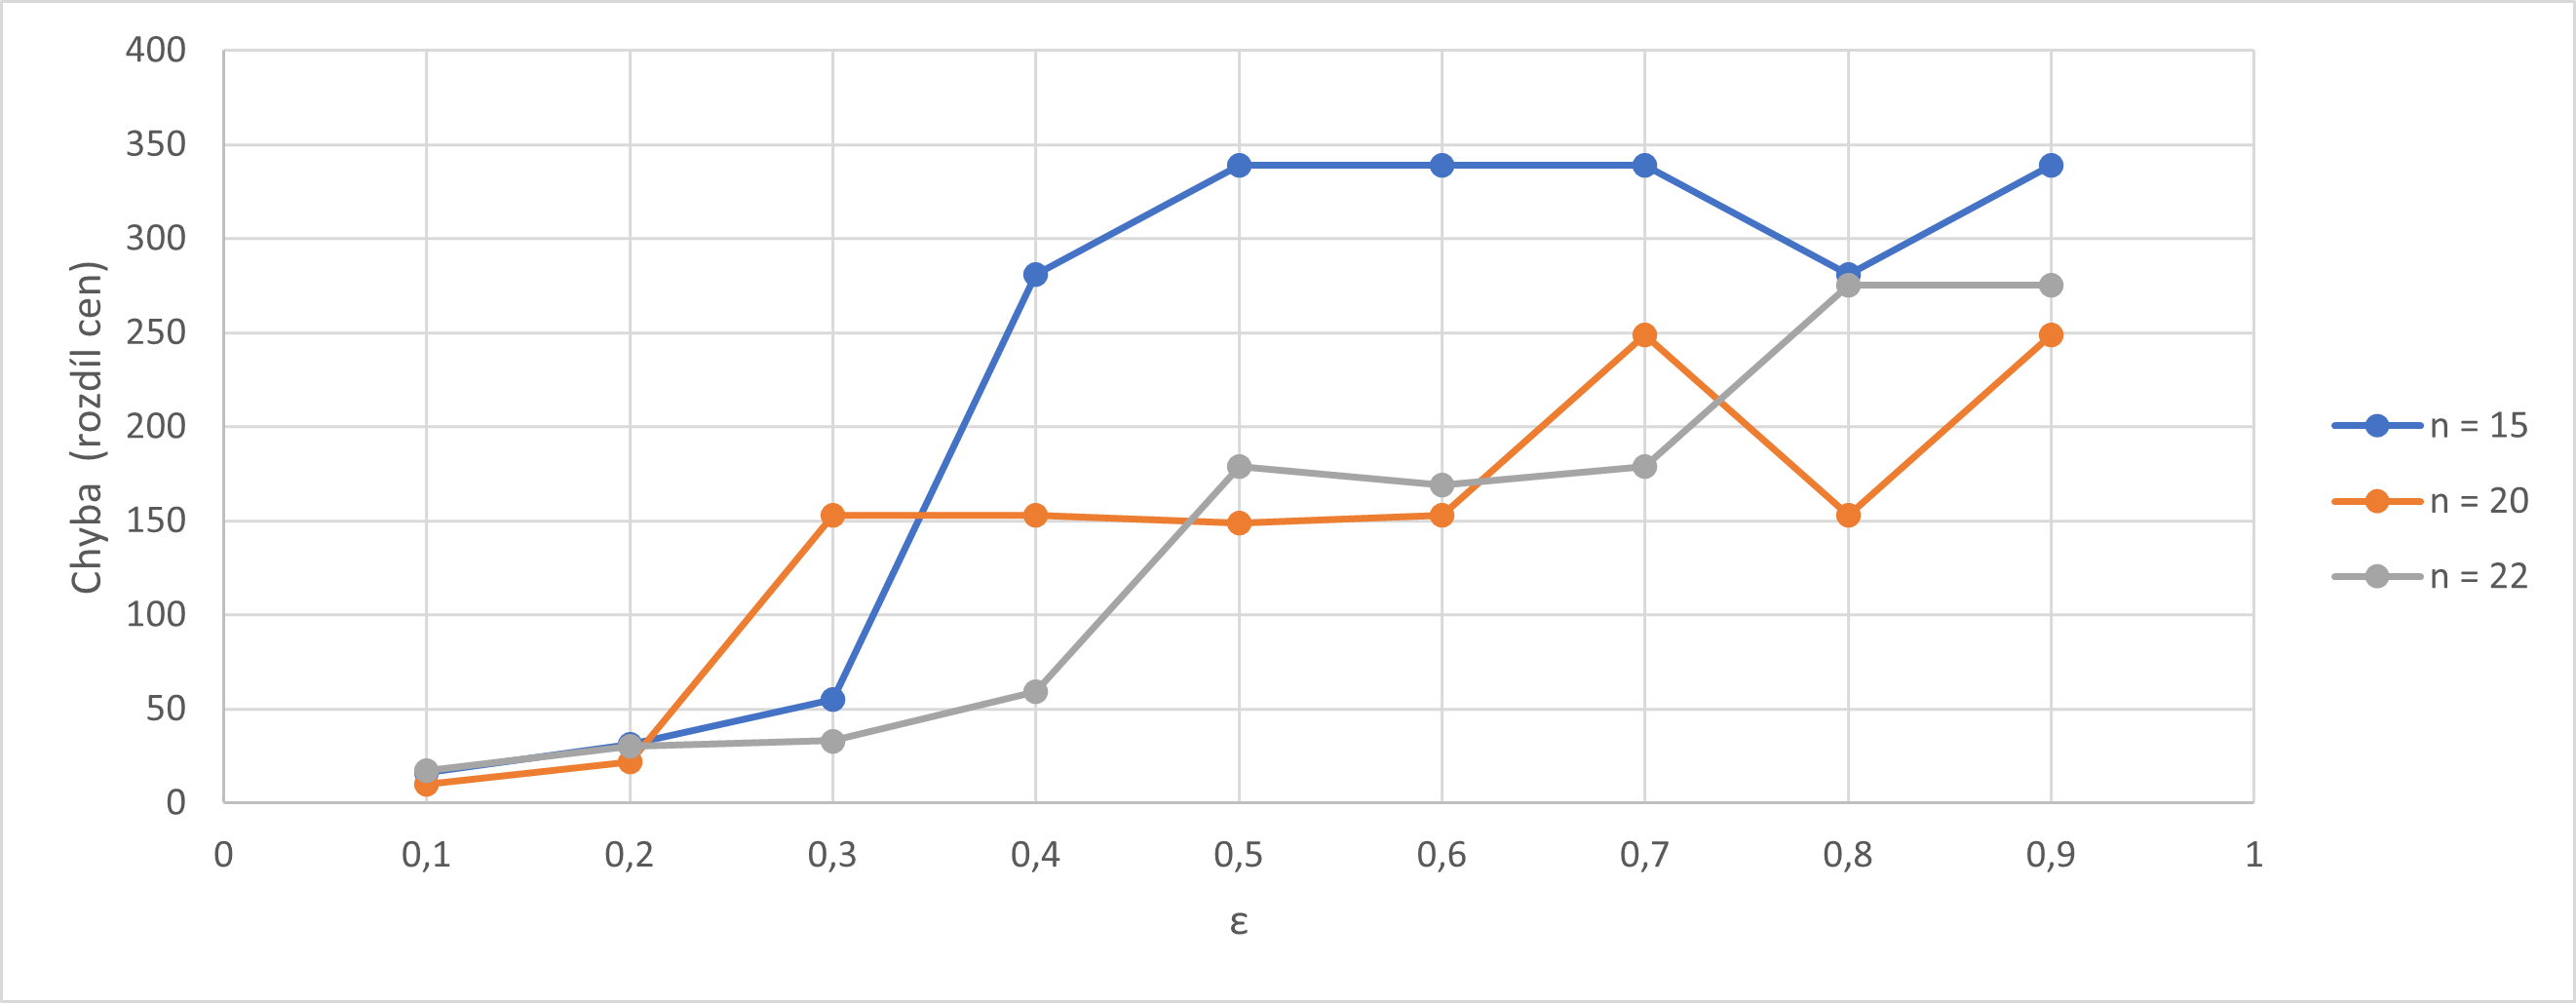
\includegraphics[width=1\textwidth, keepaspectratio]{graphs/NK/fptas/nk_fptas_eps_error.png}
    \caption{Závislost maximální reálné chyby FPTAS na $\epsilon$ (sada NK)}
    \label{fig:nk_fptas_eps_error}
\end{figure}

\begin{figure}[ht]\centering
    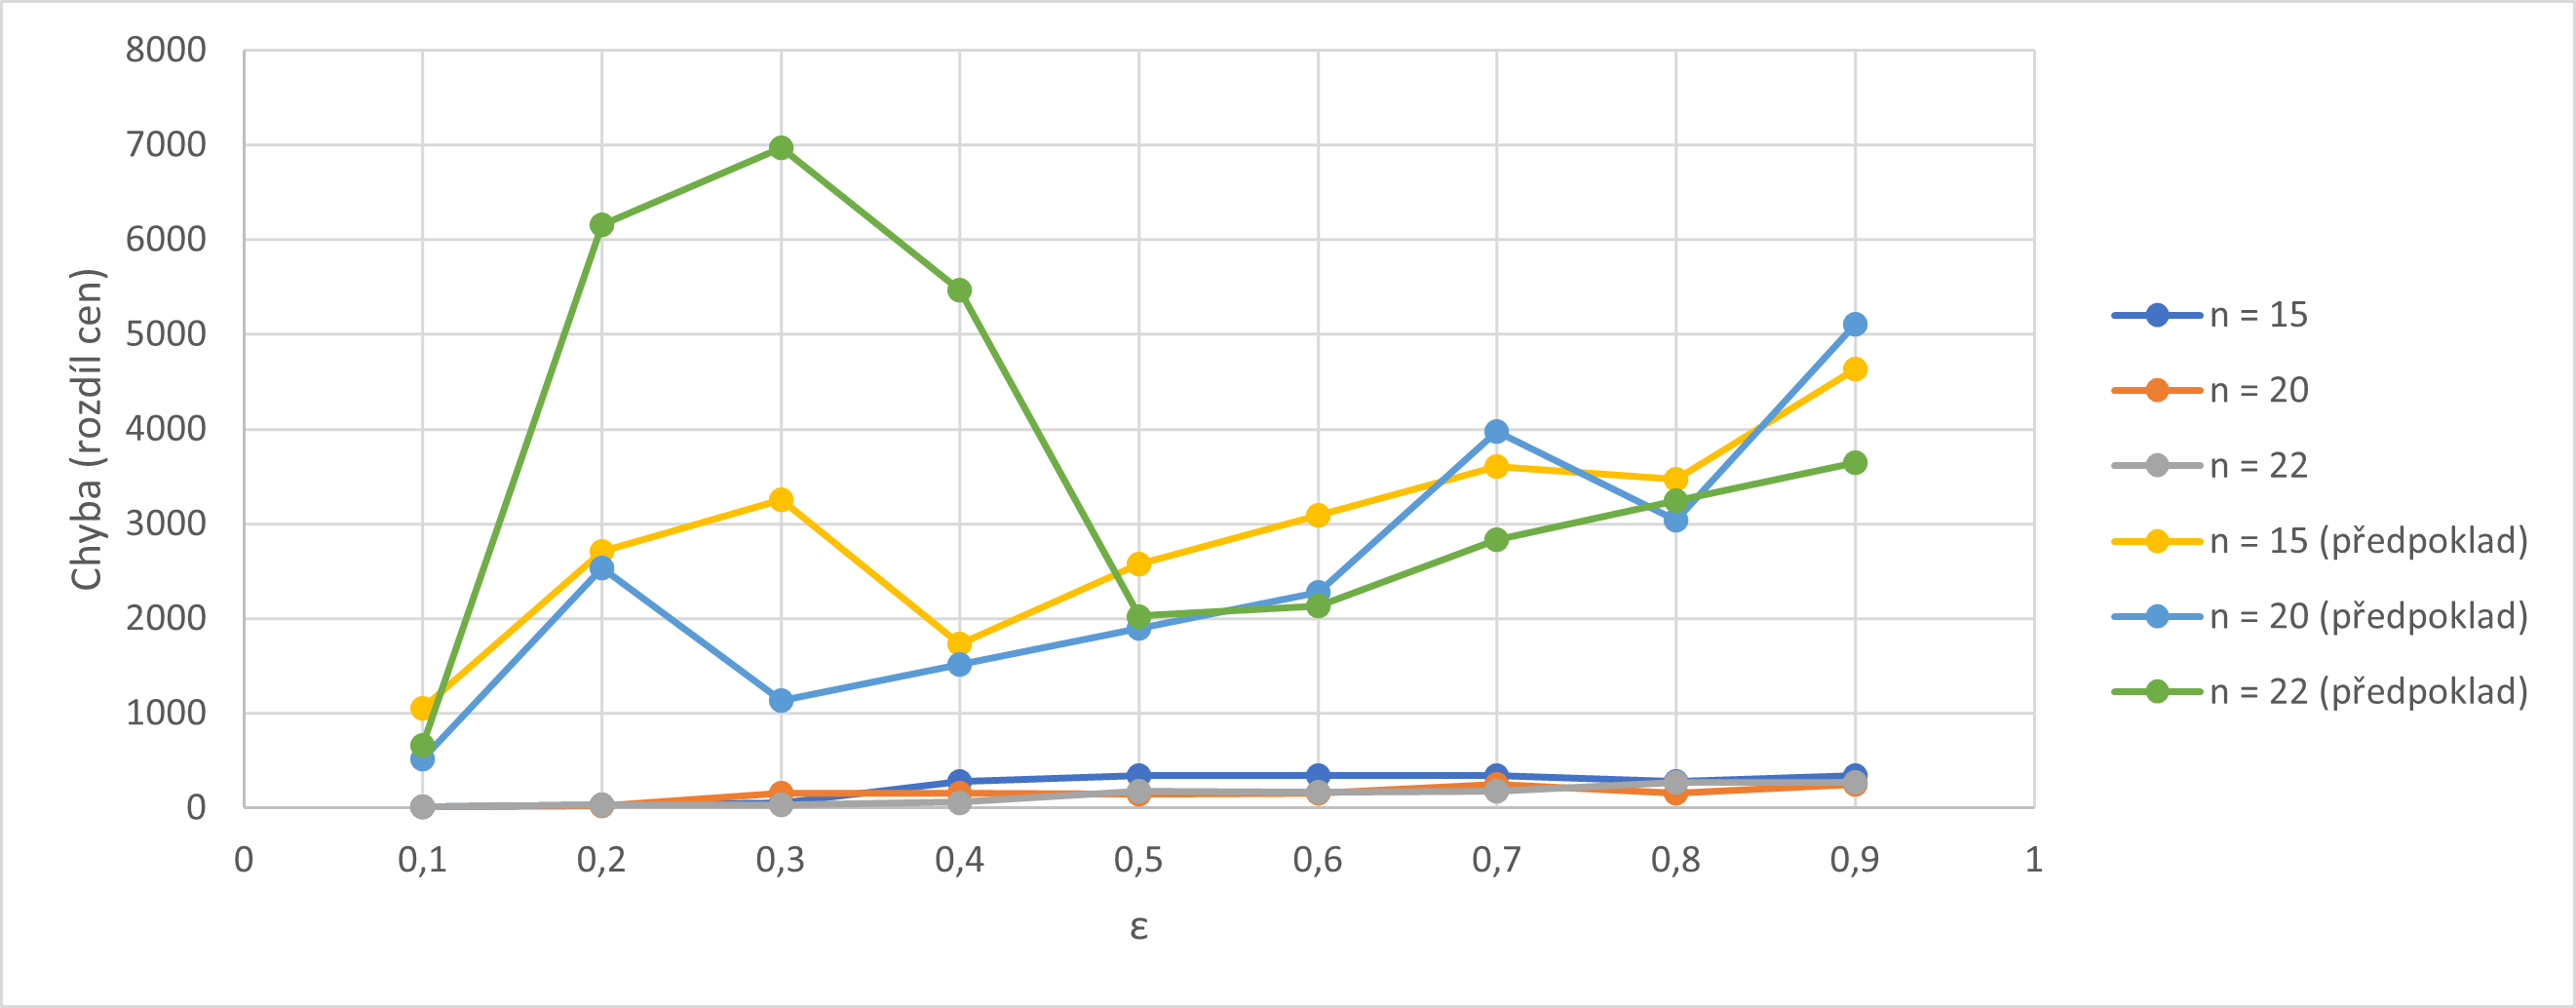
\includegraphics[width=1\textwidth, keepaspectratio]{graphs/NK/fptas/nk_fptas_eps_error_comparison.png}
    \caption{Srovnání maximální reálné chyby FPTAS s předpokládanou horní mezí v závislosti na $\epsilon$ (sada NK)}
    \label{fig:nk_fptas_eps_error_comparison}
\end{figure}

\subsection{Sada ZKC}

\subsubsection{Závislost CPU času na velikosti instance}

Naměřené údaje jsou k dispozici v tabulce \ref{tab:zkc_cpu_times}. Závislosti jsou vizualizovány v grafech \ref{fig:zkc_cpu_time_avg}, \ref{fig:zkc_cpu_time_avg_without_brute_force}, \ref{fig:zkc_cpu_time_max} a \ref{fig:zkc_cpu_time_max_without_brute_force}.

\begin{table}
    \begin{center}
         \begin{tabular}{|c | c | c | c| c | c | c | c | c|} 
         \hline
         n & BF & BF max & B\&B & B\&B max & DP & DP max & Redux & Redux max \\ [0.1ex] 
         \hline\hline
        4 & 0,001 & 0,001 & 0,001 & 0,001 & 11,178 & 18 & 0,001 & 0,001 \\
        \hline
        10 & 4,903 & 11 & 1,551 & 3 & 66,937 & 99 & 0,001 & 0,001 \\
        \hline
        15 & 128,865 & 147 & 26,685 & 52 & 149,499 & 218 & 0,001 & 0,001 \\
        \hline
        20 & 4296,931 & 6207 & 585,058 & 1318 & 305,567 & 436 & 0,001 & 0,001 \\
        \hline
        22 & 16745,207 & 18387 & 1914,046 & 4056 & 376,424 & 541 & 0,001 & 0,001 \\
        \hline
        \end{tabular}
        \caption{CPU časy dle velikosti instance (sada ZKC)}
        \label{tab:zkc_cpu_times}
    \end{center}
\end{table}

\begin{figure}[ht]\centering
    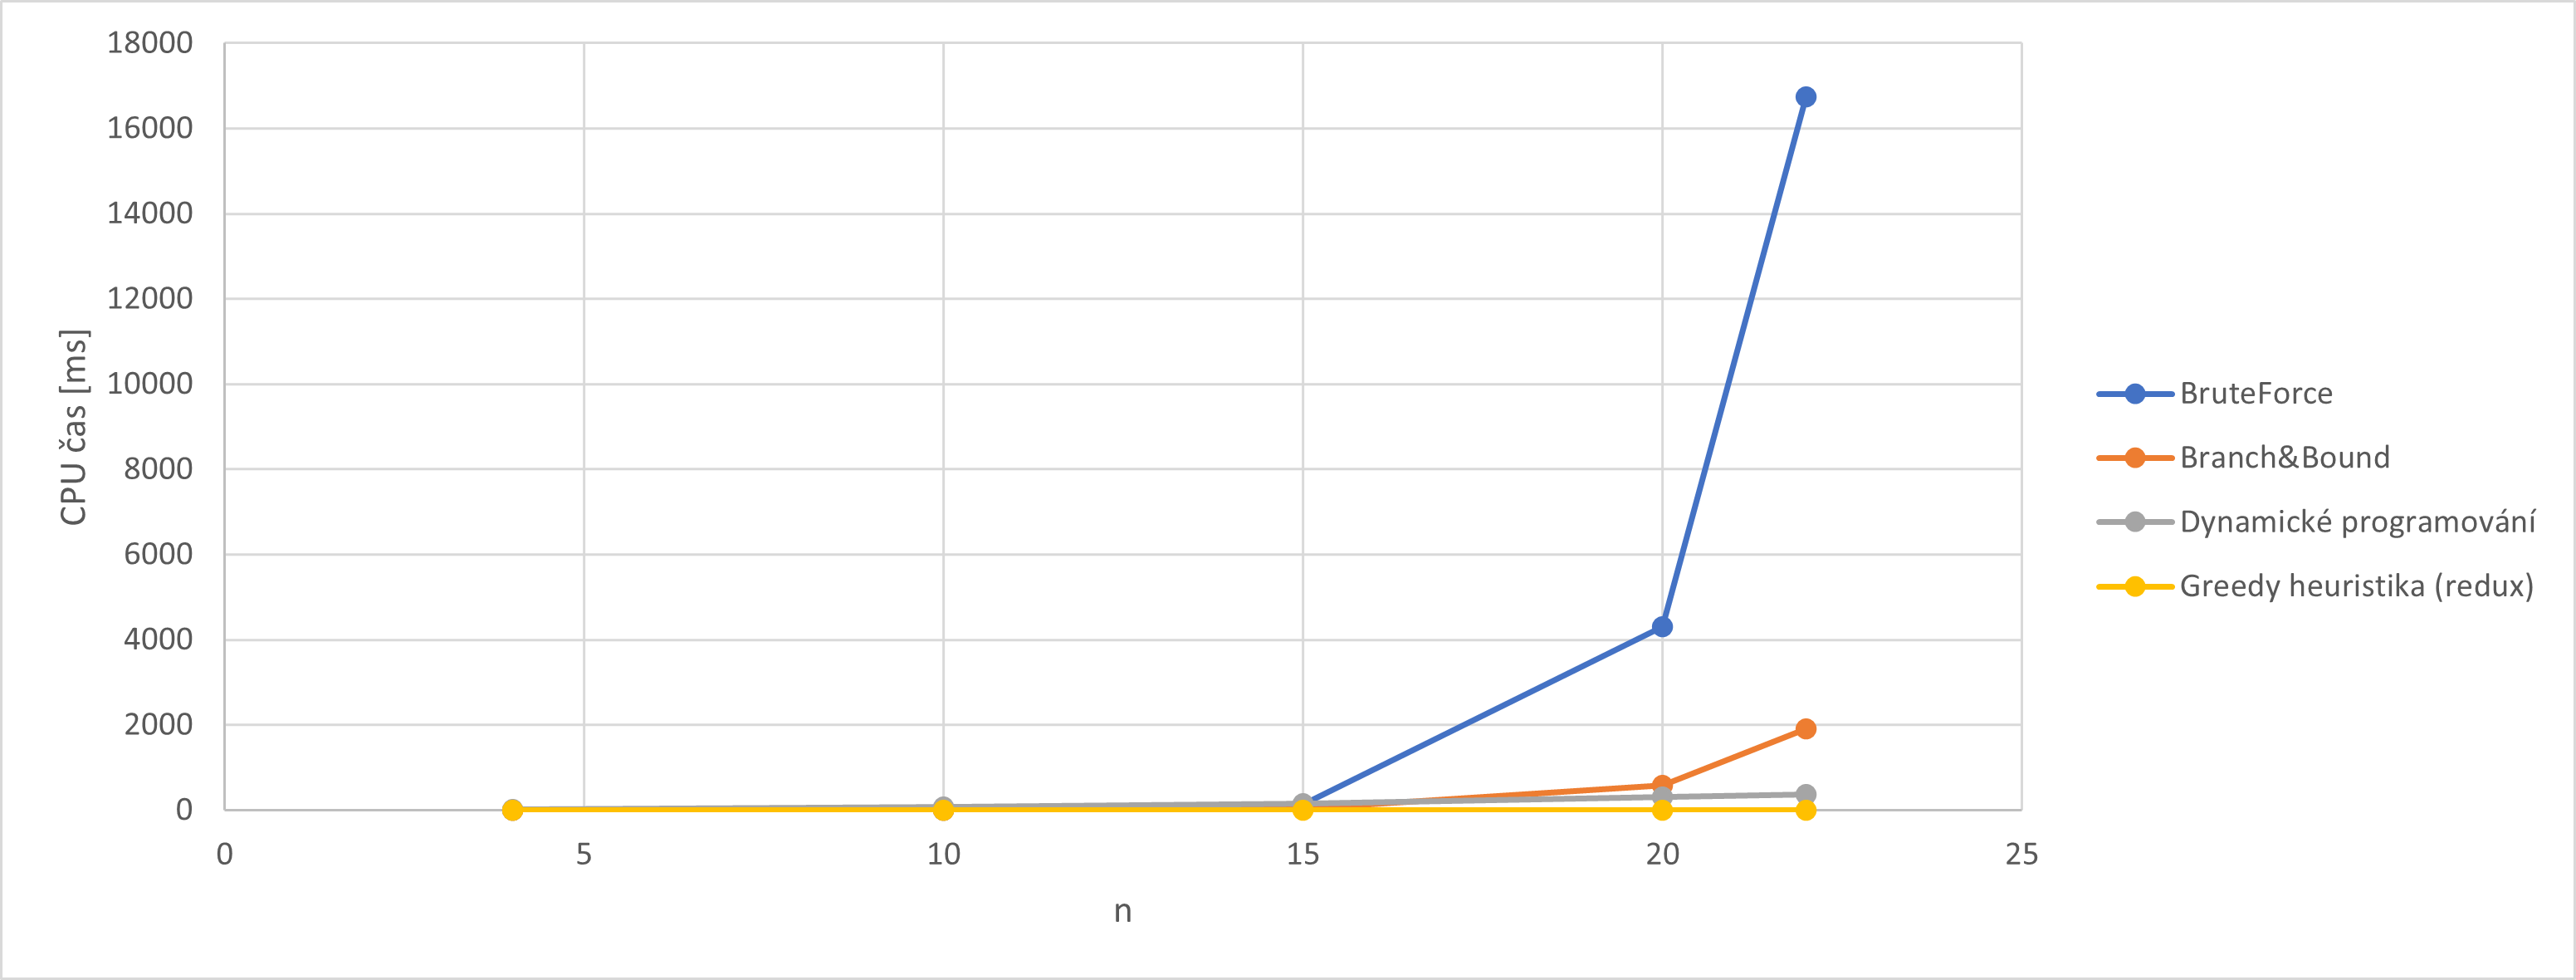
\includegraphics[width=1\textwidth, keepaspectratio]{graphs/ZKC/times/zkc_cpu_time_avg.png}
    \caption{Závislost průměrného CPU času na n (sada ZKC)}
    \label{fig:zkc_cpu_time_avg}
\end{figure}

\begin{figure}[ht]\centering
    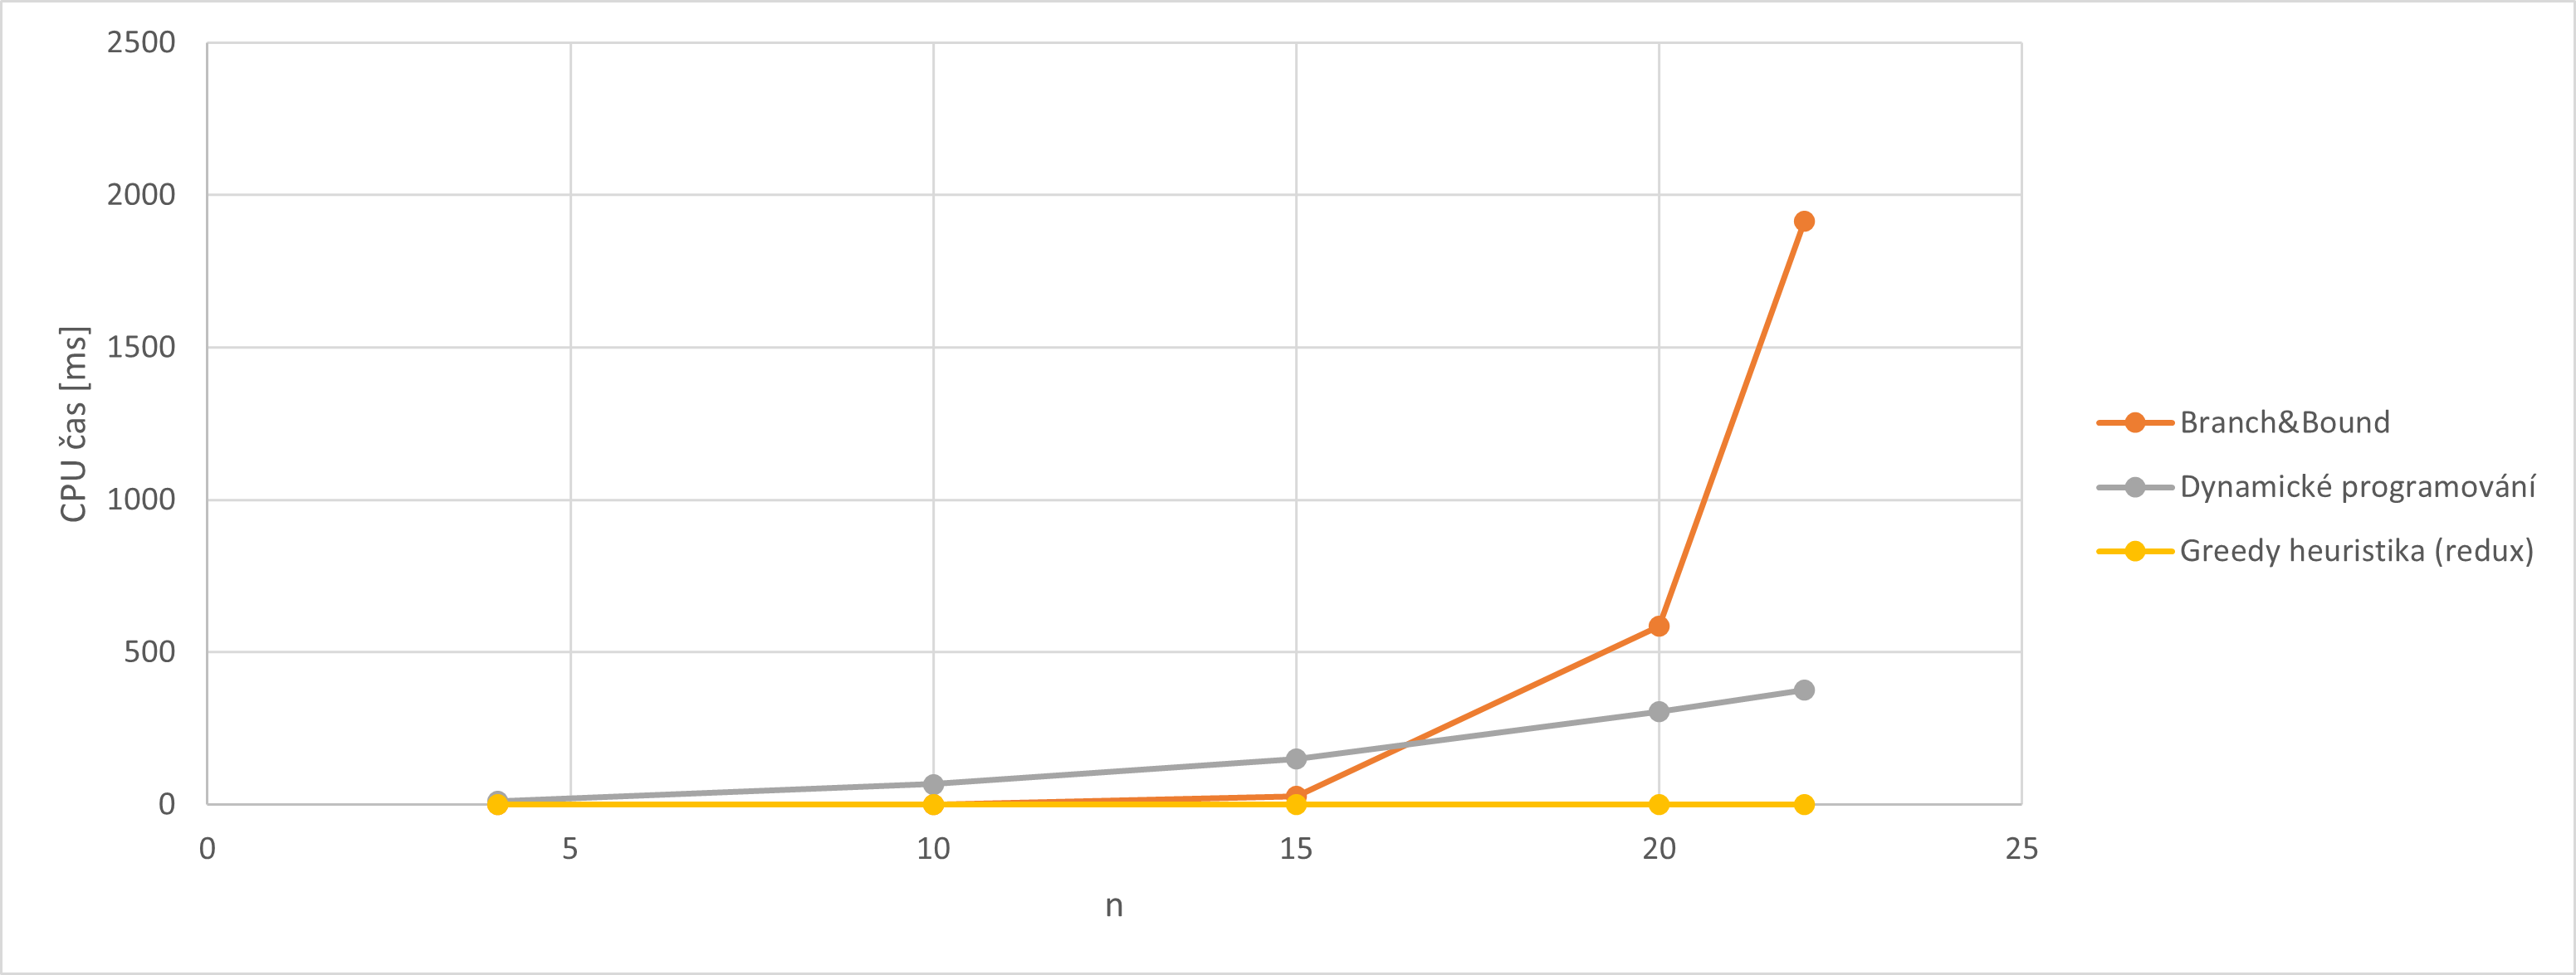
\includegraphics[width=1\textwidth, keepaspectratio]{graphs/ZKC/times/zkc_cpu_time_avg_without_brute_force.png}
    \caption{Závislost průměrného CPU času (bez BruteForce) na n (sada ZKC)}
    \label{fig:zkc_cpu_time_avg_without_brute_force}
\end{figure}

\begin{figure}[ht]\centering
    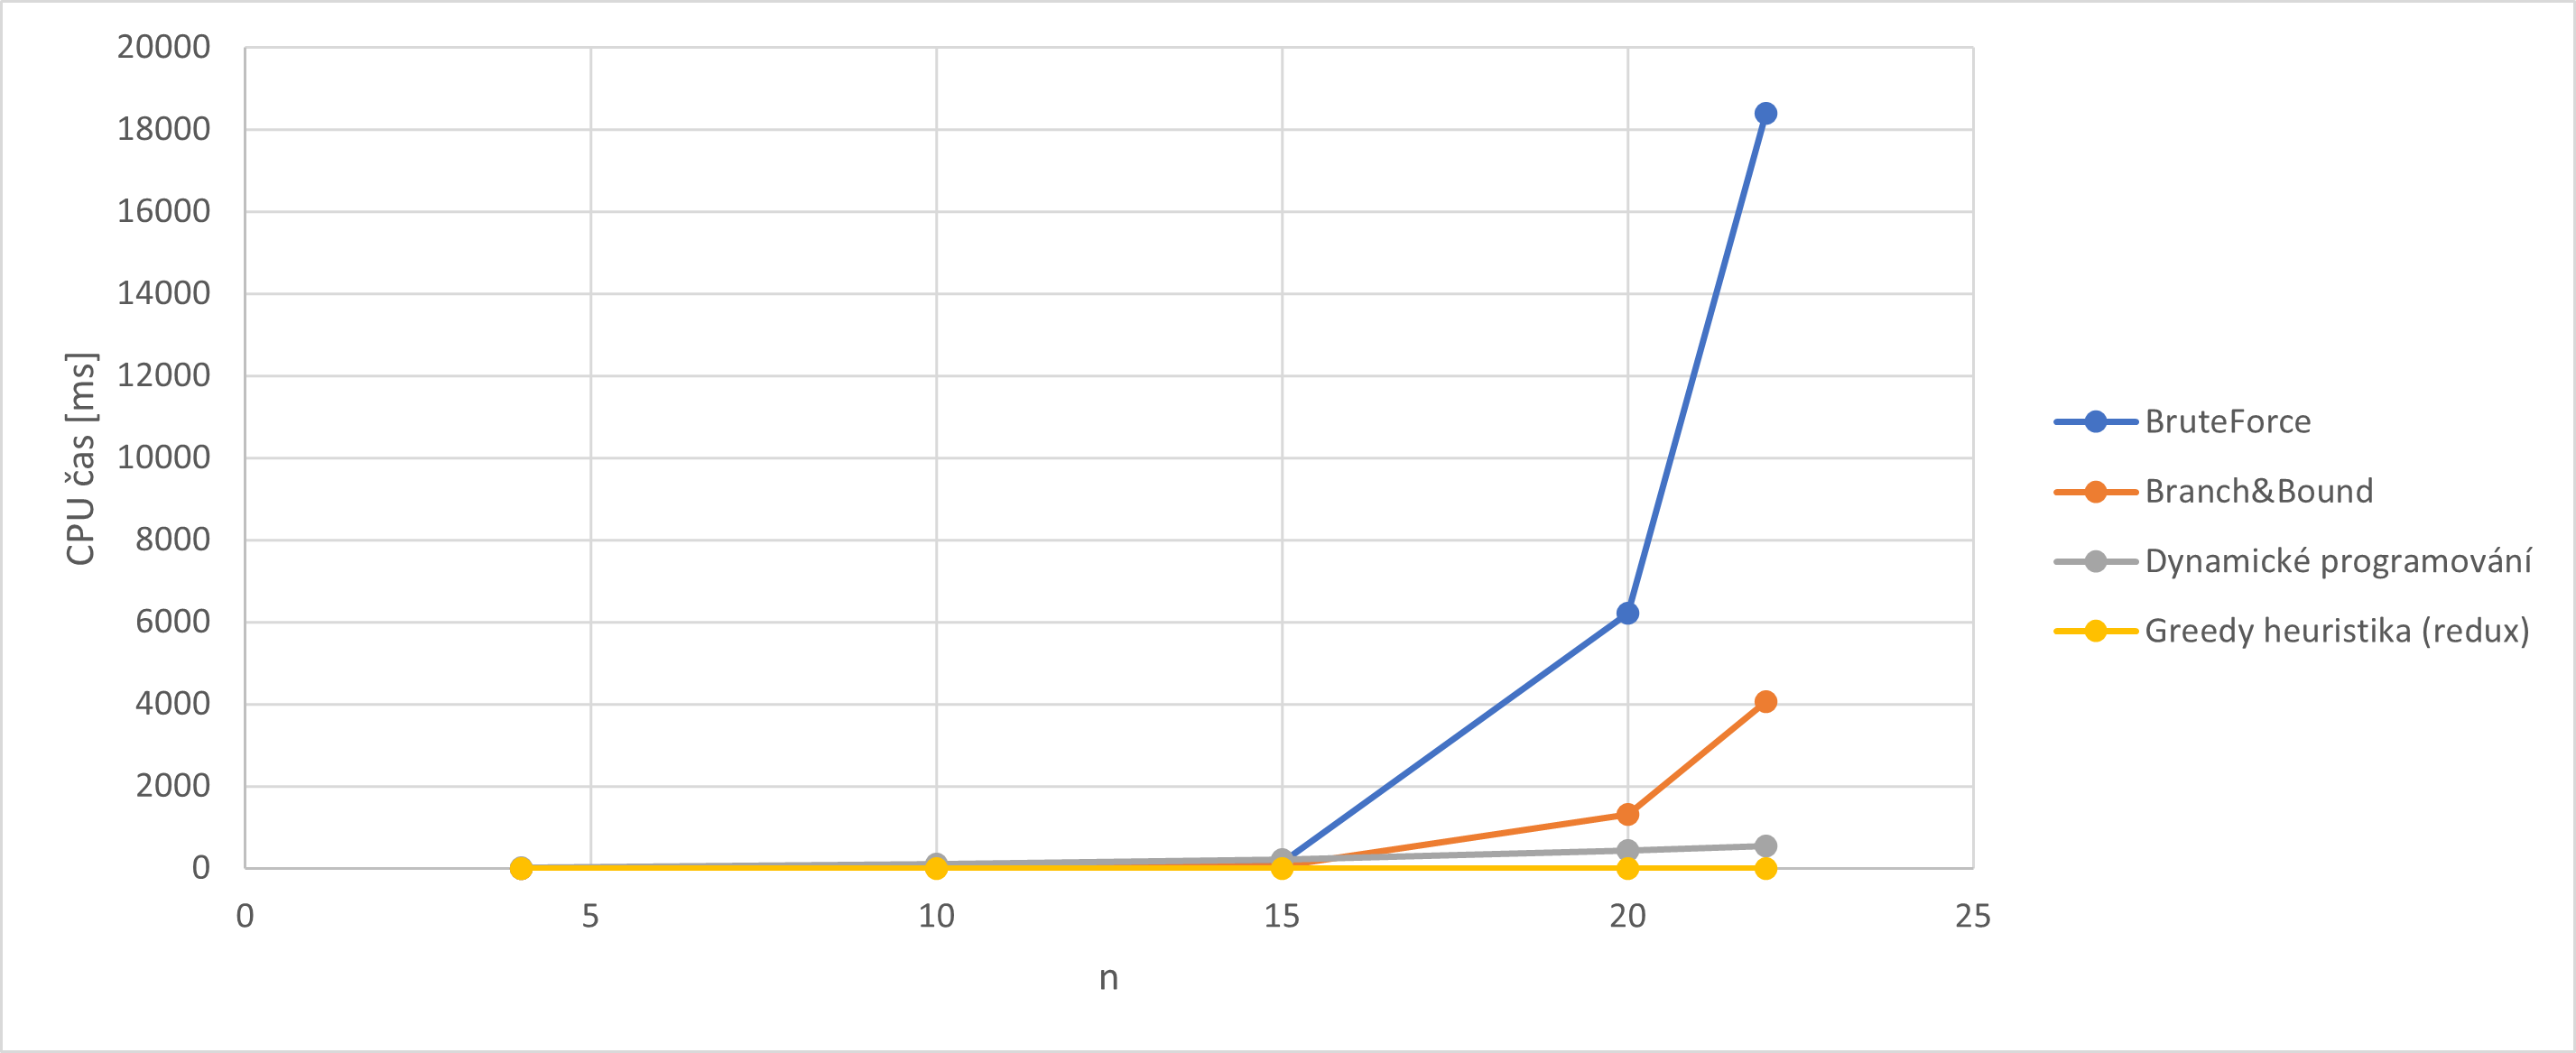
\includegraphics[width=1\textwidth, keepaspectratio]{graphs/ZKC/times/zkc_cpu_time_max.png}
    \caption{Závislost maximálního CPU času na n (sada ZKC)}
    \label{fig:zkc_cpu_time_max}
\end{figure}

\begin{figure}[ht]\centering
    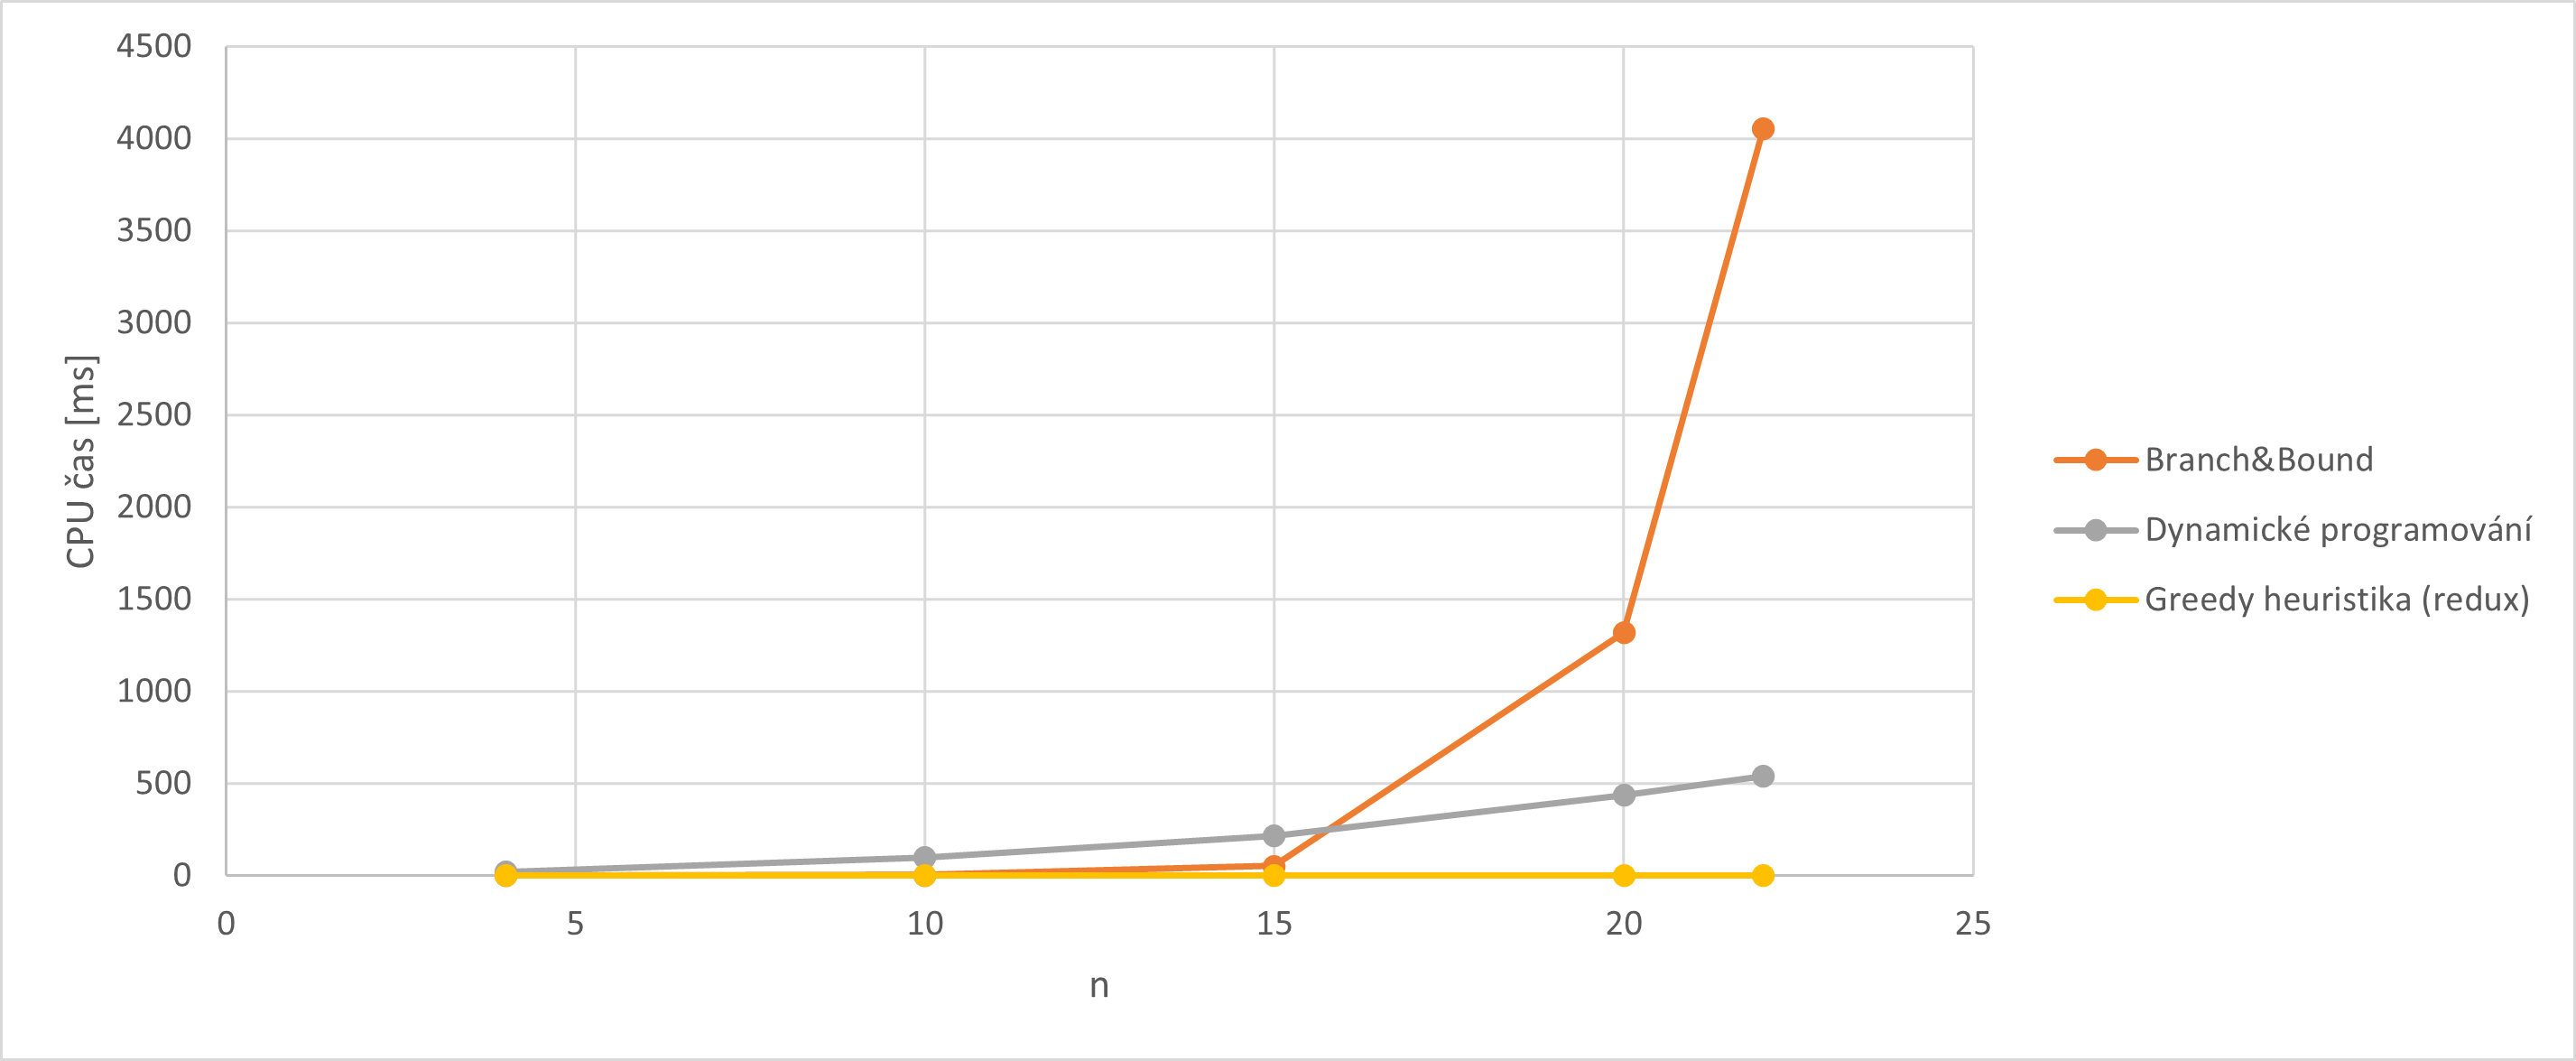
\includegraphics[width=1\textwidth, keepaspectratio]{graphs/ZKC/times/zkc_cpu_time_max_without_brute_force.png}
    \caption{Závislost maximálního CPU času (bez BruteForce) na n (sada ZKC)}
    \label{fig:zkc_cpu_time_max_without_brute_force}
\end{figure}

\subsubsection{Relativní chyby greedy heuristik}

Naměřené údaje jsou k dispozici v tabulce \ref{tab:zkc_greedy_error}. Závislosti jsou vizualizovány v grafech \ref{fig:zkc_greedy_avg} a \ref{fig:zkc_greedy_max}.

\begin{table}
    \begin{center}
         \begin{tabular}{|c | c | c | c | c|} 
         \hline
         n & Greedy & Greedy max & Greedy redux & Greedy redux max \\ [0.1ex] 
         \hline\hline
        4 & 12,940 & 49,030 & 12,430 & 43,088 \\
         \hline
        10 & 9,023 & 24,958 & 9,023 & 24,958 \\
        \hline
        15 & 6,140 & 15,486 & 6,140 & 15,486 \\
        \hline
        20 & 4,991 & 11,174 & 4,991 & 11,174 \\
        \hline
        22 & 4,267 & 10,232 & 4,267 & 10,232 \\
        \hline
        \end{tabular}
        \caption{Relativní chyby greedy heuristik (sada ZKC)} \label{tab:zkc_greedy_error}
    \end{center}
\end{table}

\begin{figure}[ht]\centering
    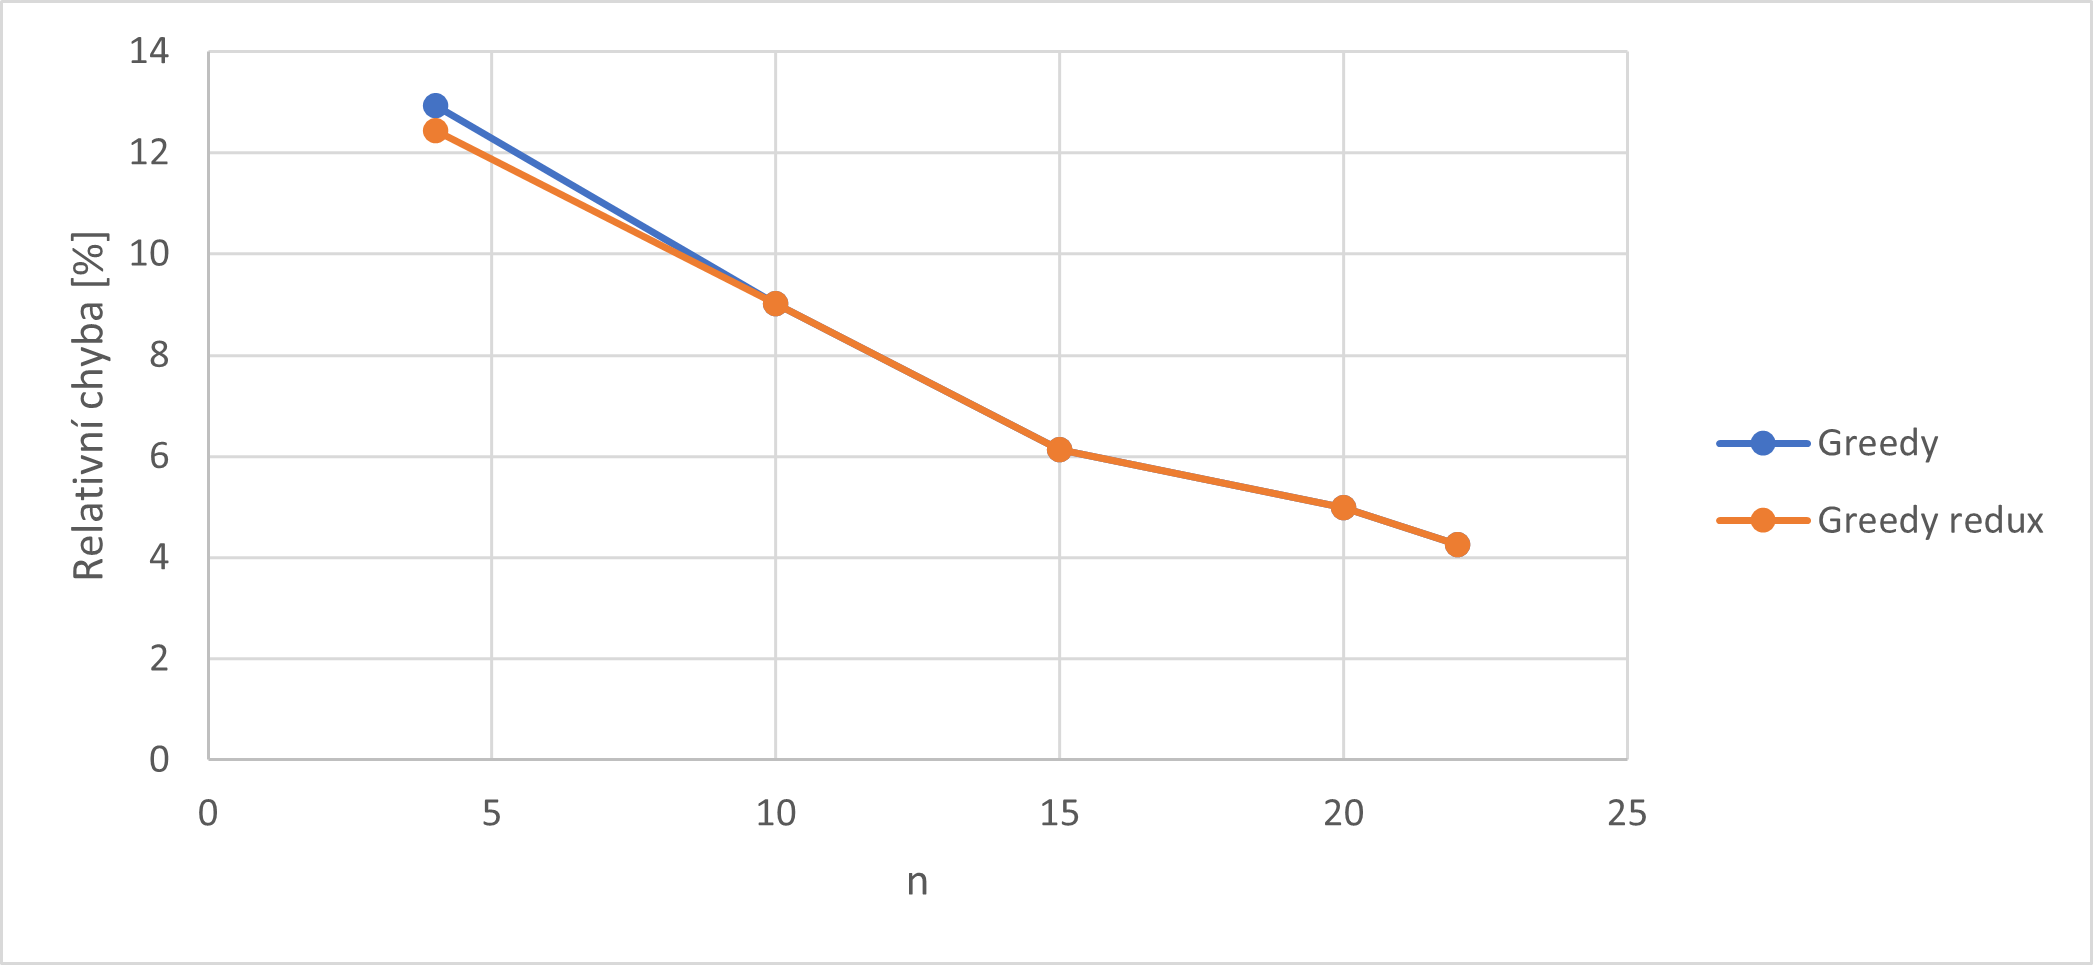
\includegraphics[width=1\textwidth, keepaspectratio]{graphs/ZKC/heuristics/zkc_greedy_avg.png}
    \caption{Průměrná relativní chyba heuristik (sada ZKC)}
    \label{fig:zkc_greedy_avg}
\end{figure}

\begin{figure}[ht]\centering
    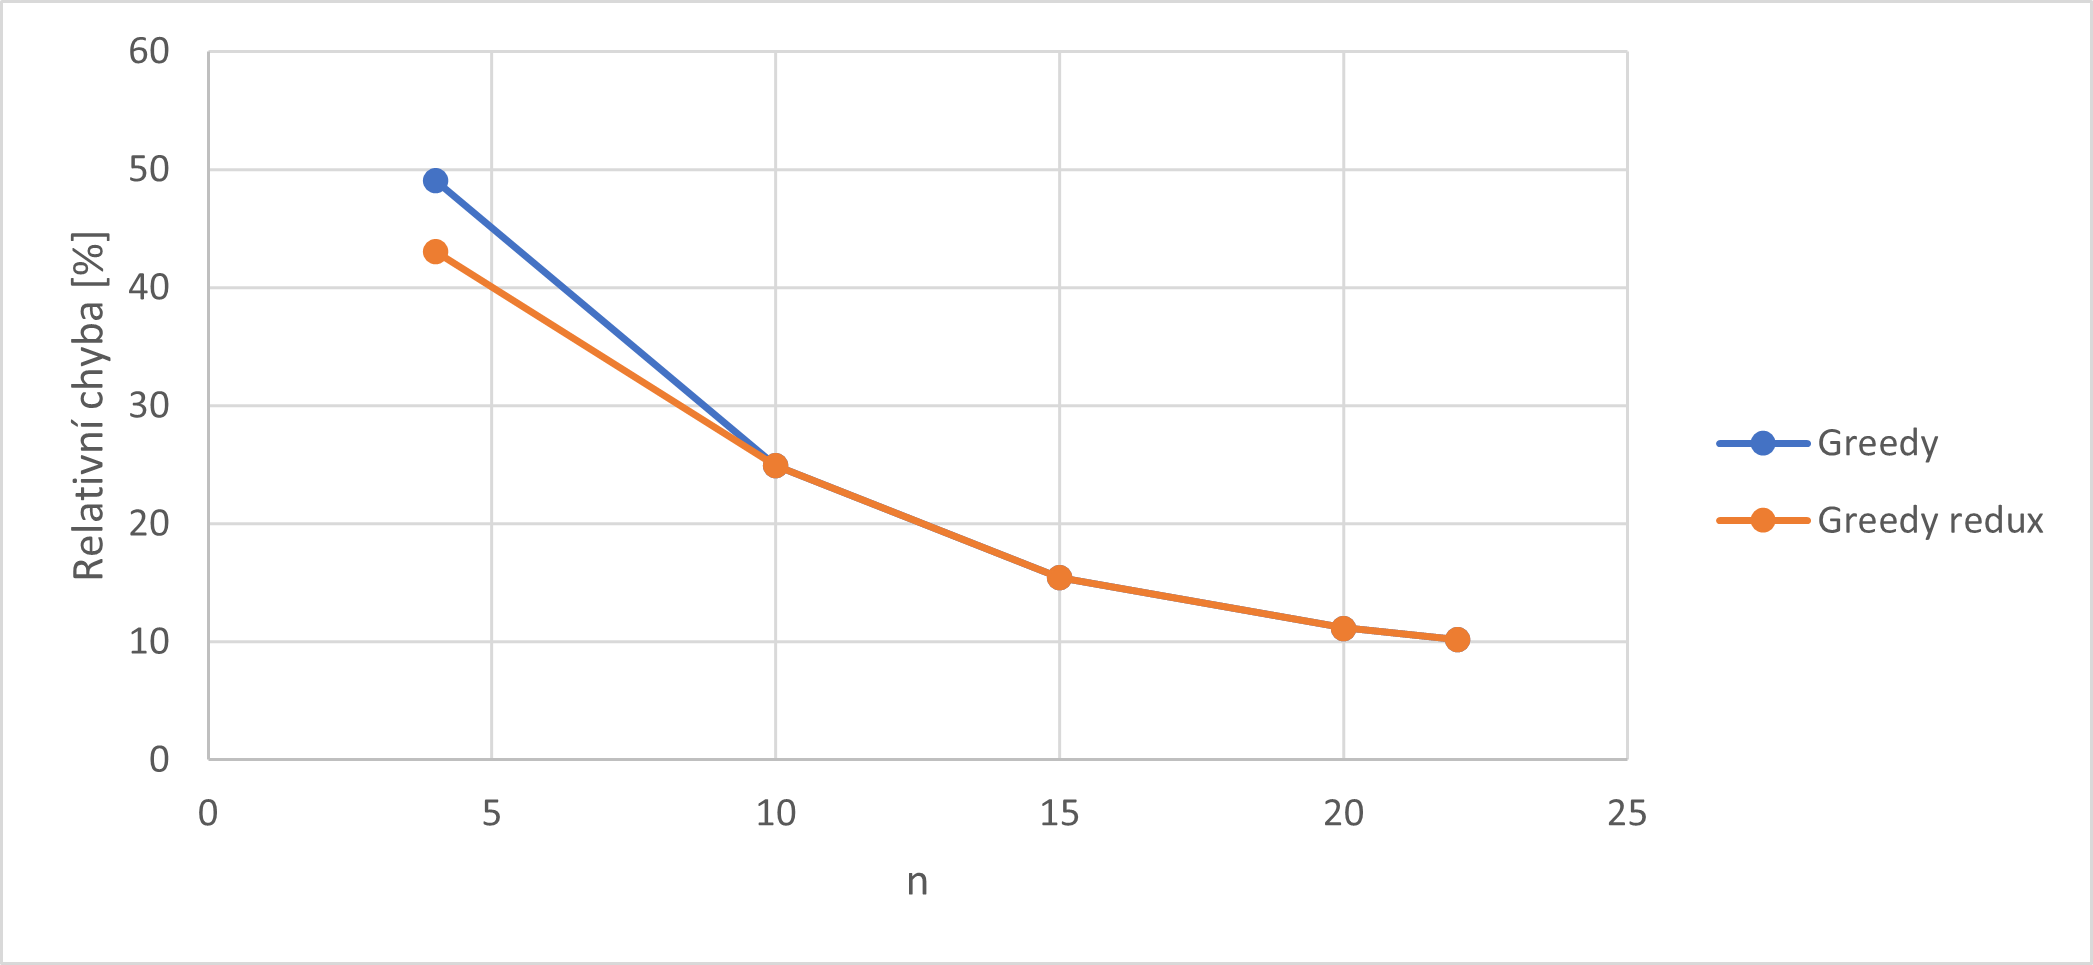
\includegraphics[width=1\textwidth, keepaspectratio]{graphs/ZKC/heuristics/zkc_greedy_max.png}
    \caption{Maximální relativní chyba heuristik (sada ZKC)}
    \label{fig:zkc_greedy_max}
\end{figure}

\subsubsection{CPU čas a chyby algoritmu FPTAS}

Naměřené hodnoty CPU času jsou k dispozici v tabulce \ref{tab:zkc_fptas_eps_times}. Závislosti CPU času jsou vizualizovány v grafech \ref{fig:zkc_fptas_eps_time_avg} a \ref{fig:zkc_fptas_eps_time_max}.
Naměřené hodnoty chyb jsou k dispozici v tabulce \ref{tab:zkc_fptas_eps_error}. Závislosti reálné chyby FPTAS algoritmu jsou vizualizovány v grafu \ref{fig:zkc_fptas_eps_error}. Srovnání reálné a maximální předpokládané chyby algoritmu FPTAS je k dispozici v grafu~\ref{fig:zkc_fptas_eps_error_comparison}.

\begin{table}
    \begin{center}
         \begin{tabular}{|c | c | c | c | c | c | c|} 
         \hline
         $\epsilon$ & n=15 & n=15 (max) & n=20 & n=20 (max) & n=22 & n=22 (max) \\ [0.1ex] 
         \hline\hline
        0,1 & 10,192 & 16 & 23,464 & 34 & 29,930 & 39 \\
        \hline
        0,2 & 5,208 & 8 & 11,869 & 19 & 14,975 & 32 \\
        \hline
        0,3 & 3,539 & 7 & 8,167 & 35 & 10,019 & 14 \\
        \hline
        0,4 & 2,774 & 4 & 5,825 & 13 & 7,518 & 11 \\
        \hline
        0,5 & 2,122 & 4 & 4,514 & 6 & 6,046 & 10,001 \\
        \hline
        0,6 & 1,958 & 3 & 3,778 & 6 & 5,018 & 9 \\
        \hline
        0,7 & 1,661 & 3 & 3,168 & 5 & 4,251 & 7 \\
        \hline
        0,8 & 1,210 & 2 & 2,965 & 9 & 3,790 & 5 \\
        \hline
        0,9 & 1,027 & 2 & 2,541 & 5 & 3,301 & 7 \\
        \hline
        \end{tabular}
        \caption{CPU časy algoritmus FPTAS v závilosti na $\epsilon$ (sada ZKC)} \label{tab:zkc_fptas_eps_times}
    \end{center}
\end{table}

\begin{figure}[ht]\centering
    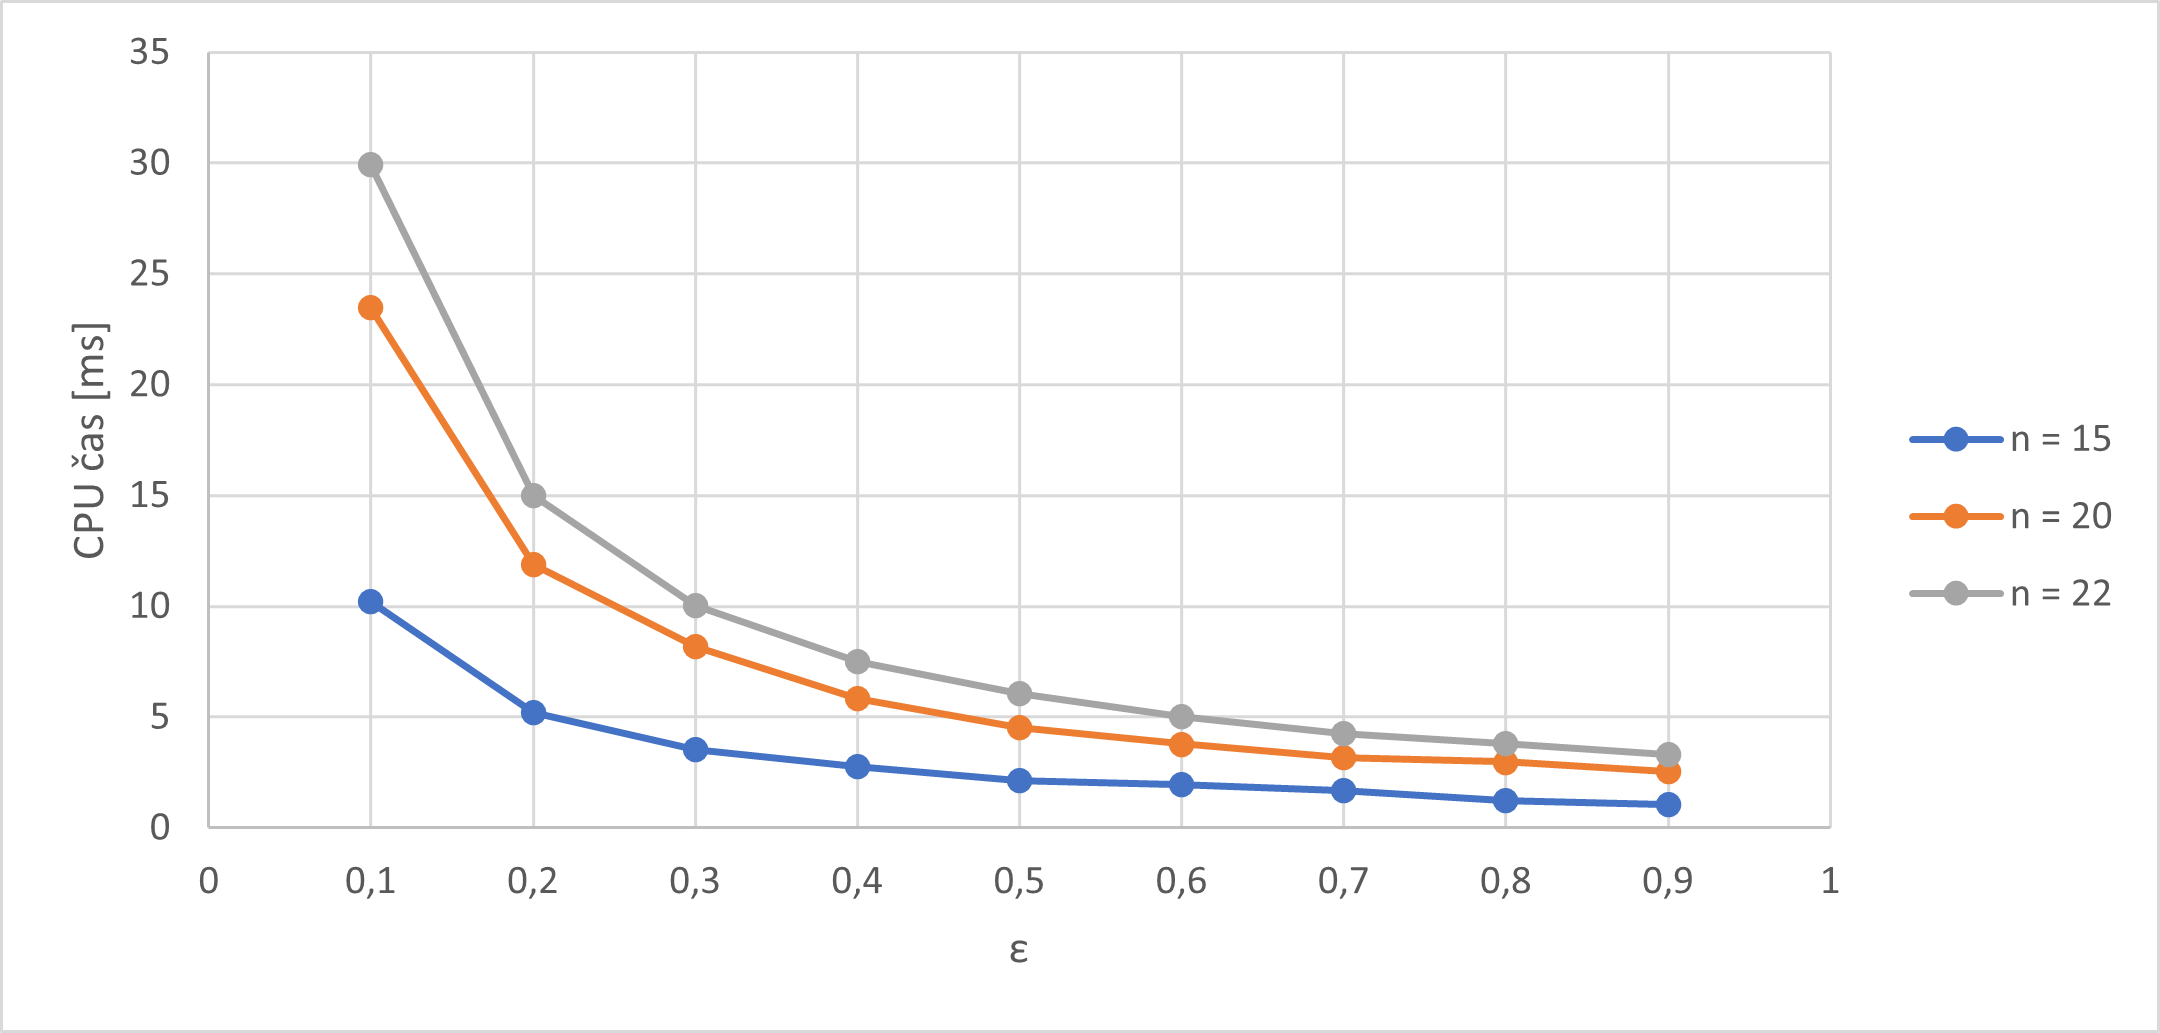
\includegraphics[width=1\textwidth, keepaspectratio]{graphs/ZKC/fptas/zkc_fptas_time_eps_avg.png}
    \caption{Závislost průměrného CPU času FPTAS na $\epsilon$ (sada ZKC)}
    \label{fig:zkc_fptas_eps_time_avg}
\end{figure}

\begin{figure}[ht]\centering
    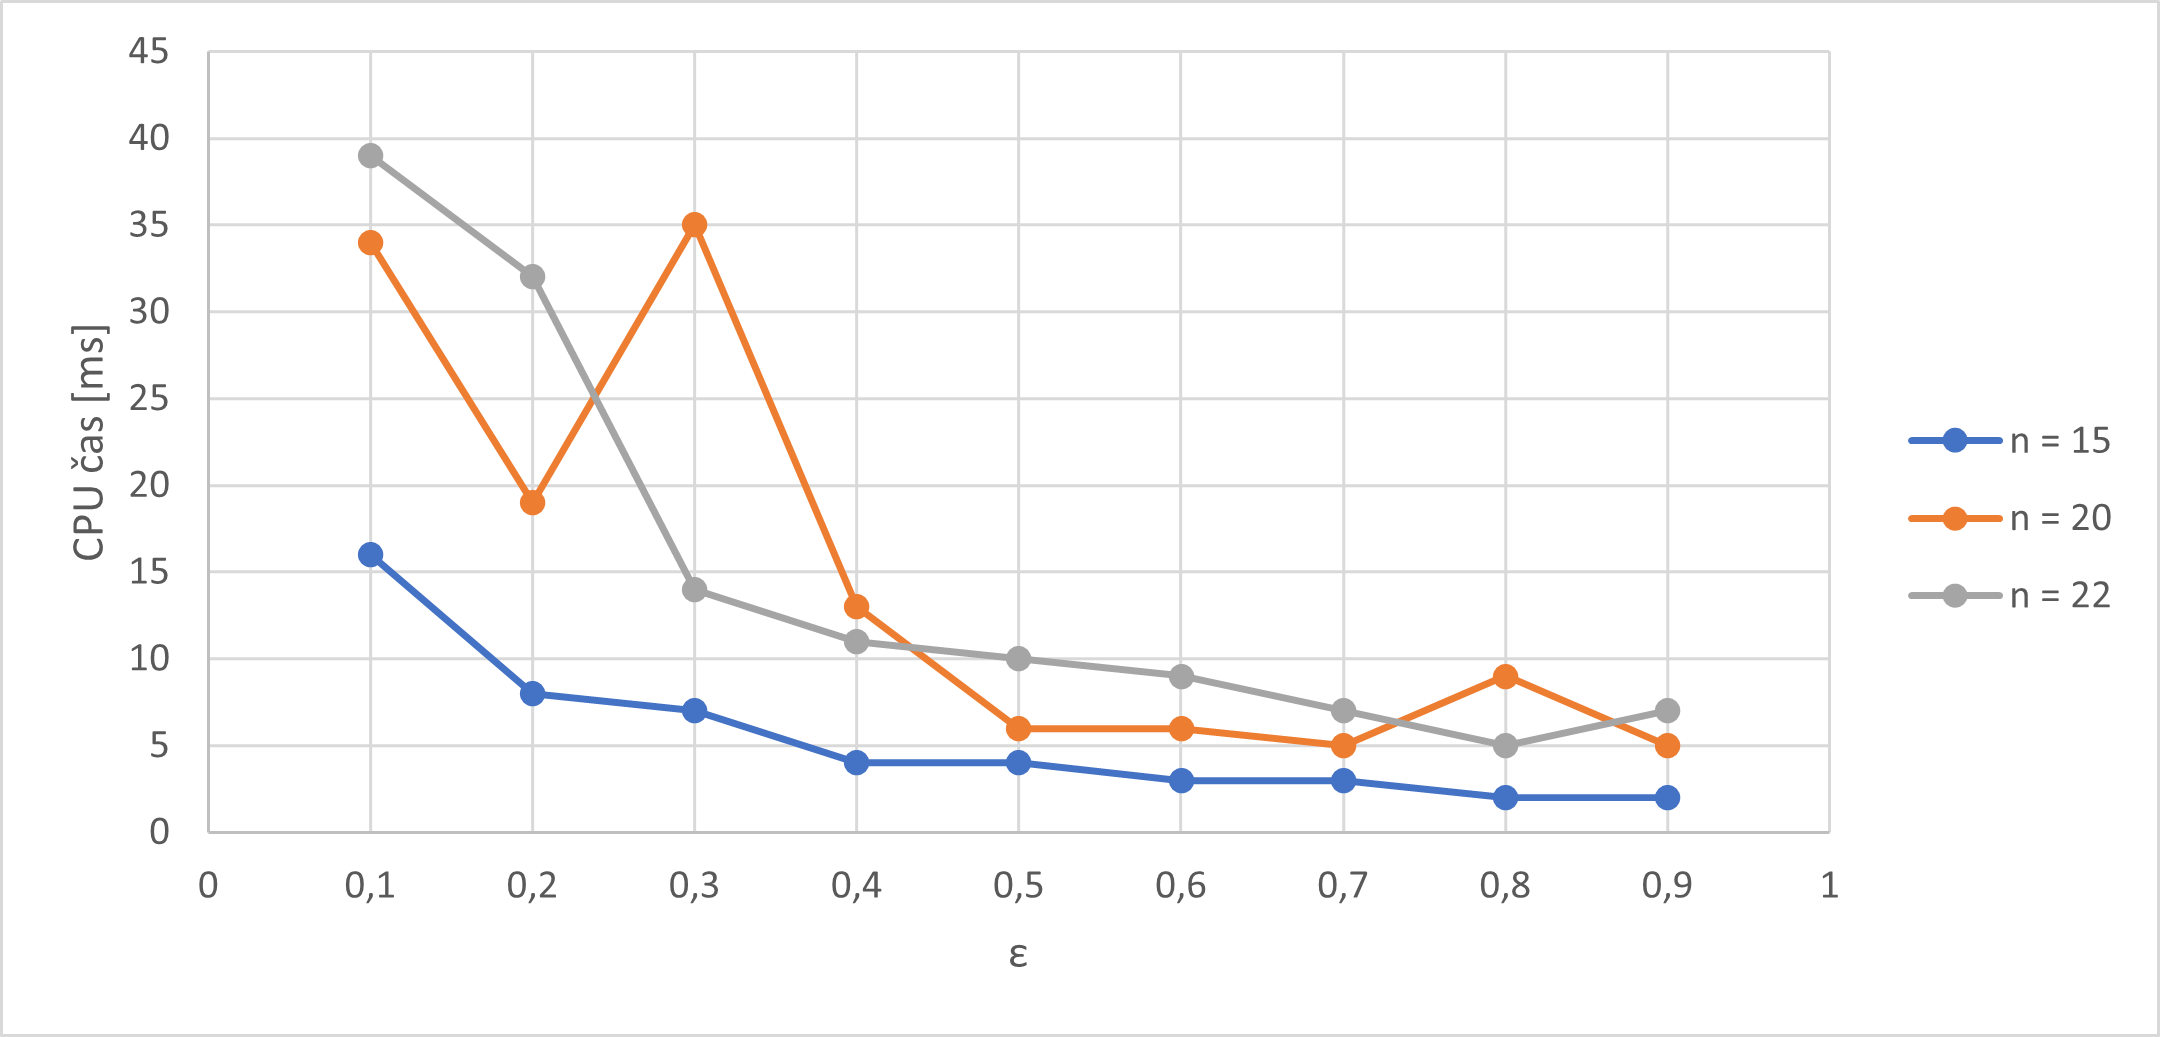
\includegraphics[width=1\textwidth, keepaspectratio]{graphs/ZKC/fptas/zkc_fptas_time_eps_max.png}
    \caption{Závislost maximálního CPU času FPTAS na $\epsilon$ (sada ZKC)}
    \label{fig:zkc_fptas_eps_time_max}
\end{figure}

\begin{table}
    \begin{center}
         \begin{tabular}{|c | c | c | c | c | c | c|} 
         \hline
         $\epsilon$ & n=15 & n=15 (předpoklad) & n=20 & n=20 (předpoklad) & n=22 & n=22 (předpoklad) \\ [0.1ex] 
         \hline\hline
        0,1 & 24 & 1361,700 & 21 & 1728,800 & 22 & 1900,800 \\
        \hline
        0,2 & 58 & 2669,200 & 40 & 3473,400 & 41 & 3635,400 \\
        \hline
        0,3 & 76 & 4600,800 & 58 & 5037,300 & 56 & 6203,400 \\
        \hline
        0,4 & 95 & 5752 & 80 & 7744 & 73 & 7669,600 \\
        \hline
        0,5 & 114 & 7091 & 115 & 7716,500 & 84 & 10244 \\
        \hline
        0,6 & 137 & 7878,600 & 106 & 10820,400 & 91 & 11479,200 \\
        \hline
        0,7 & 262 & 9751 & 246 & 13005,300 & 97 & 12247,900 \\
        \hline
        0,8 & 312 & 9704 & 304 & 14772,800 & 142 & 18288,800 \\
        \hline
        0,9 & 405 & 12574,800 & 299 & 17987,400 & 267 & 18257,400 \\
        \hline
        \end{tabular}
        \caption{Maximální reálné a předpokládané chyby algoritmu FPTAS v závislosti na $\epsilon$ (sada ZKC)} \label{tab:zkc_fptas_eps_error}
    \end{center}
\end{table}

\begin{figure}[ht]\centering
    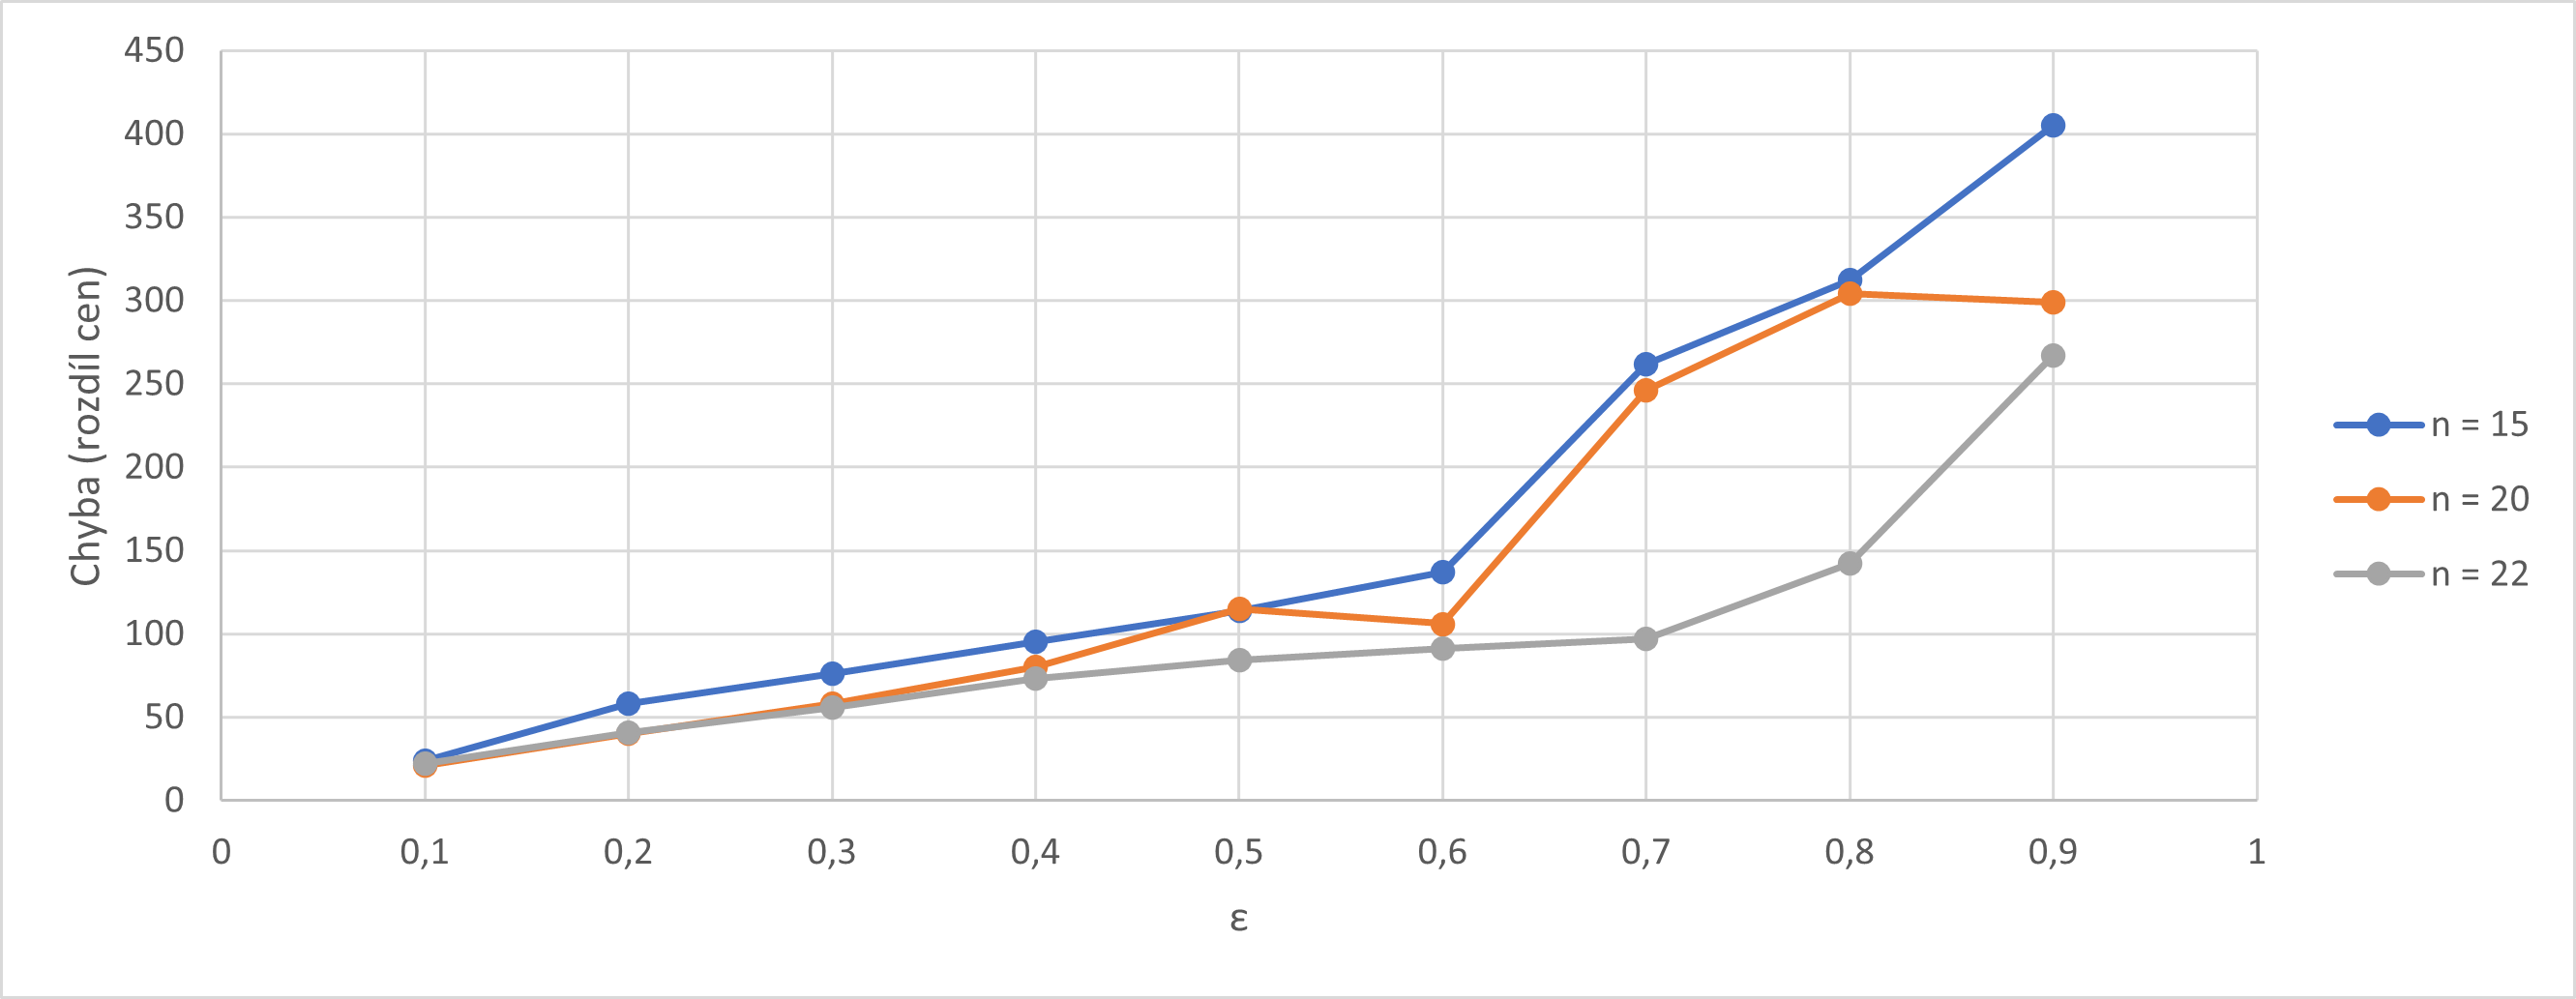
\includegraphics[width=1\textwidth, keepaspectratio]{graphs/ZKC/fptas/zkc_fptas_eps_error.png}
    \caption{Závislost maximální reálné chyby FPTAS na $\epsilon$ (sada ZKC)}
    \label{fig:zkc_fptas_eps_error}
\end{figure}

\begin{figure}[ht]\centering
    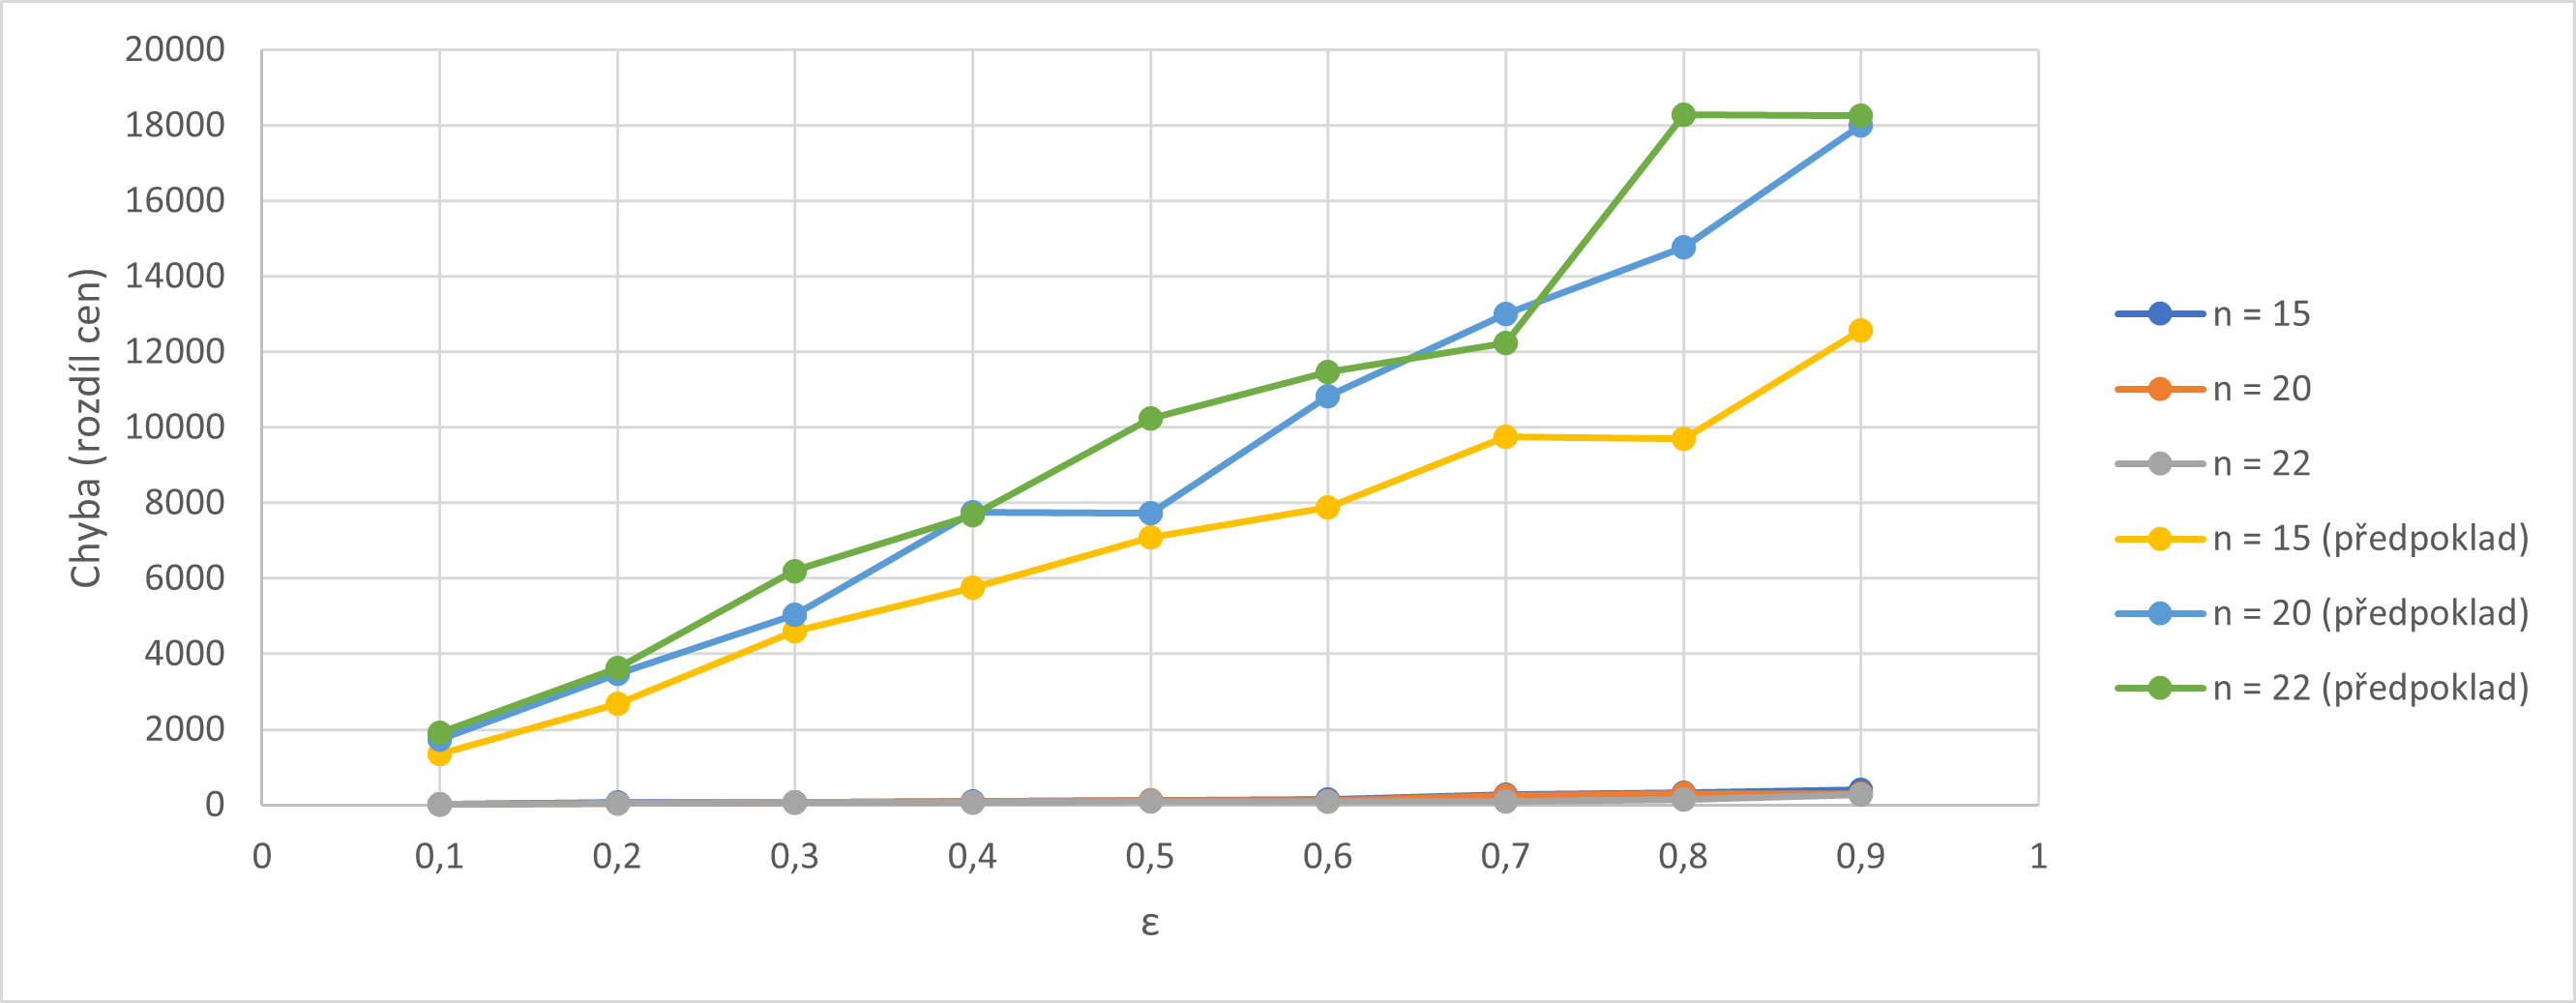
\includegraphics[width=1\textwidth, keepaspectratio]{graphs/ZKC/fptas/zkc_fptas_eps_error_comparison.png}
    \caption{Srovnání maximální reálné chyby FPTAS s předpokládanou horní mezí v závislosti na $\epsilon$ (sada ZKC)}
    \label{fig:zkc_fptas_eps_error_comparison}
\end{figure}

\subsection{Sada ZKW}

\subsubsection{Závislost CPU času na velikosti instance}

Naměřené údaje jsou k dispozici v tabulce \ref{tab:zkw_cpu_times}. Závislosti jsou vizualizovány v grafech \ref{fig:zkw_cpu_time_avg}, \ref{fig:zkw_cpu_time_avg_without_brute_force}, \ref{fig:zkw_cpu_time_max} a \ref{fig:zkw_cpu_time_max_without_brute_force}.

\begin{table}
    \begin{center}
         \begin{tabular}{|c | c | c | c| c | c | c | c | c|} 
         \hline
         n & BF & BF max & B\&B & B\&B max & DP & DP max & Redux & Redux max \\ [0.1ex] 
         \hline\hline
        4 & 0,003 & 2 & 0,001 & 1 & 19,741 & 595 & 0,001 & 0,001 \\
        \hline
        10 & 4,093 & 5 & 0,319 & 4 & 68,516 & 1267 & 0,001 & 0,001 \\
        \hline
        15 & 127,344 & 135 & 1,604 & 61 & 103,989 & 313 & 0,001 & 0,001 \\
        \hline
        20 & 4142,649 & 4845 & 2,463 & 29 & 159,615 & 411 & 0,001 & 0,001 \\
        \hline
        22 & 16832,565 & 17792 & 6,241 & 227 & 216,236 & 2077 & 0,001 & 0,001 \\
        \hline
        \end{tabular}
        \caption{CPU časy dle velikosti instance (sada ZKW)}
        \label{tab:zkw_cpu_times}
    \end{center}
\end{table}

\begin{figure}[ht]\centering
    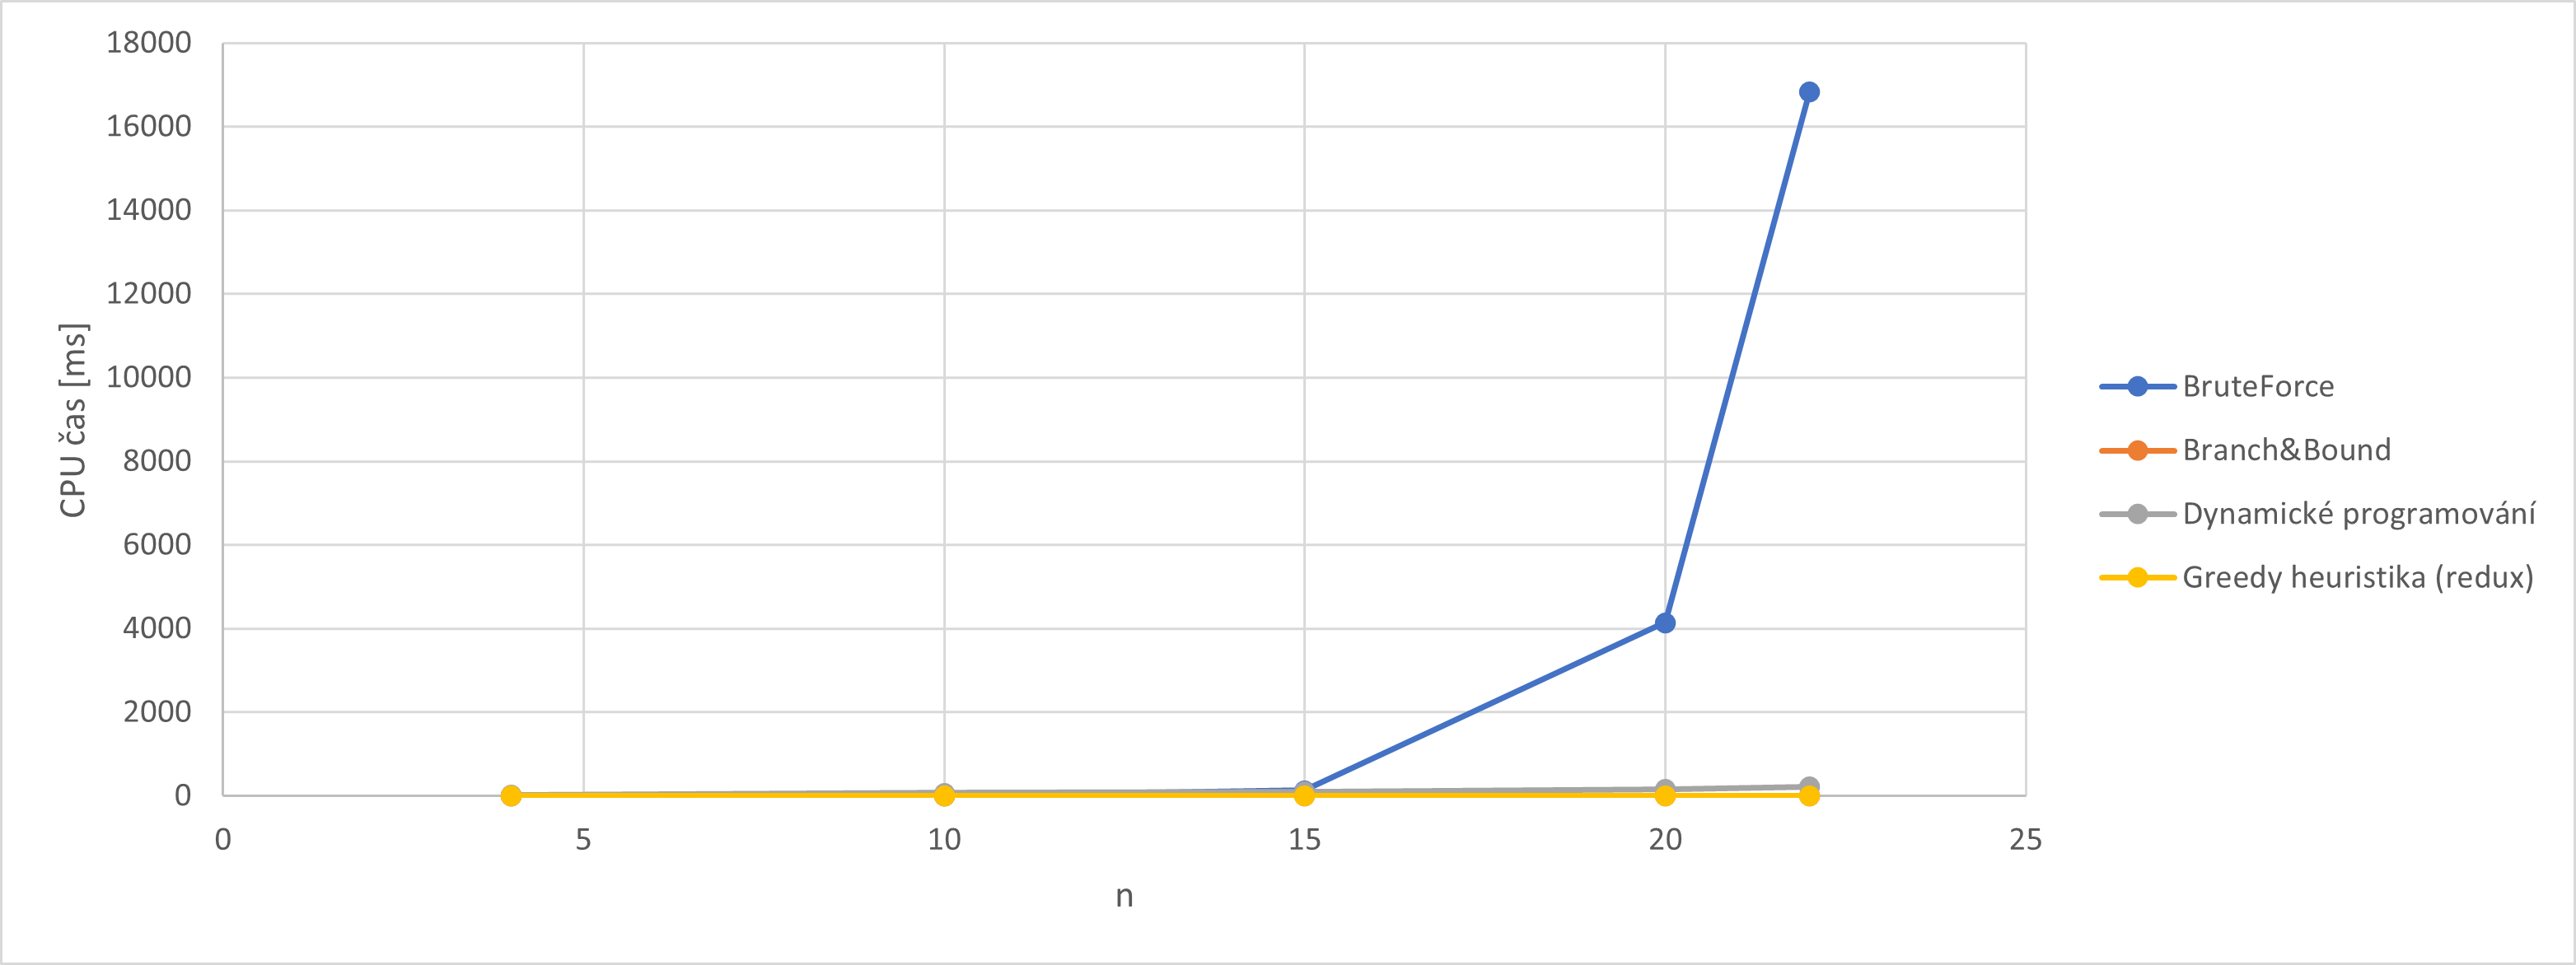
\includegraphics[width=1\textwidth, keepaspectratio]{graphs/ZKW/times/zkw_cpu_time_avg.png}
    \caption{Závislost průměrného CPU času na n (sada ZKW)}
    \label{fig:zkw_cpu_time_avg}
\end{figure}

\begin{figure}[ht]\centering
    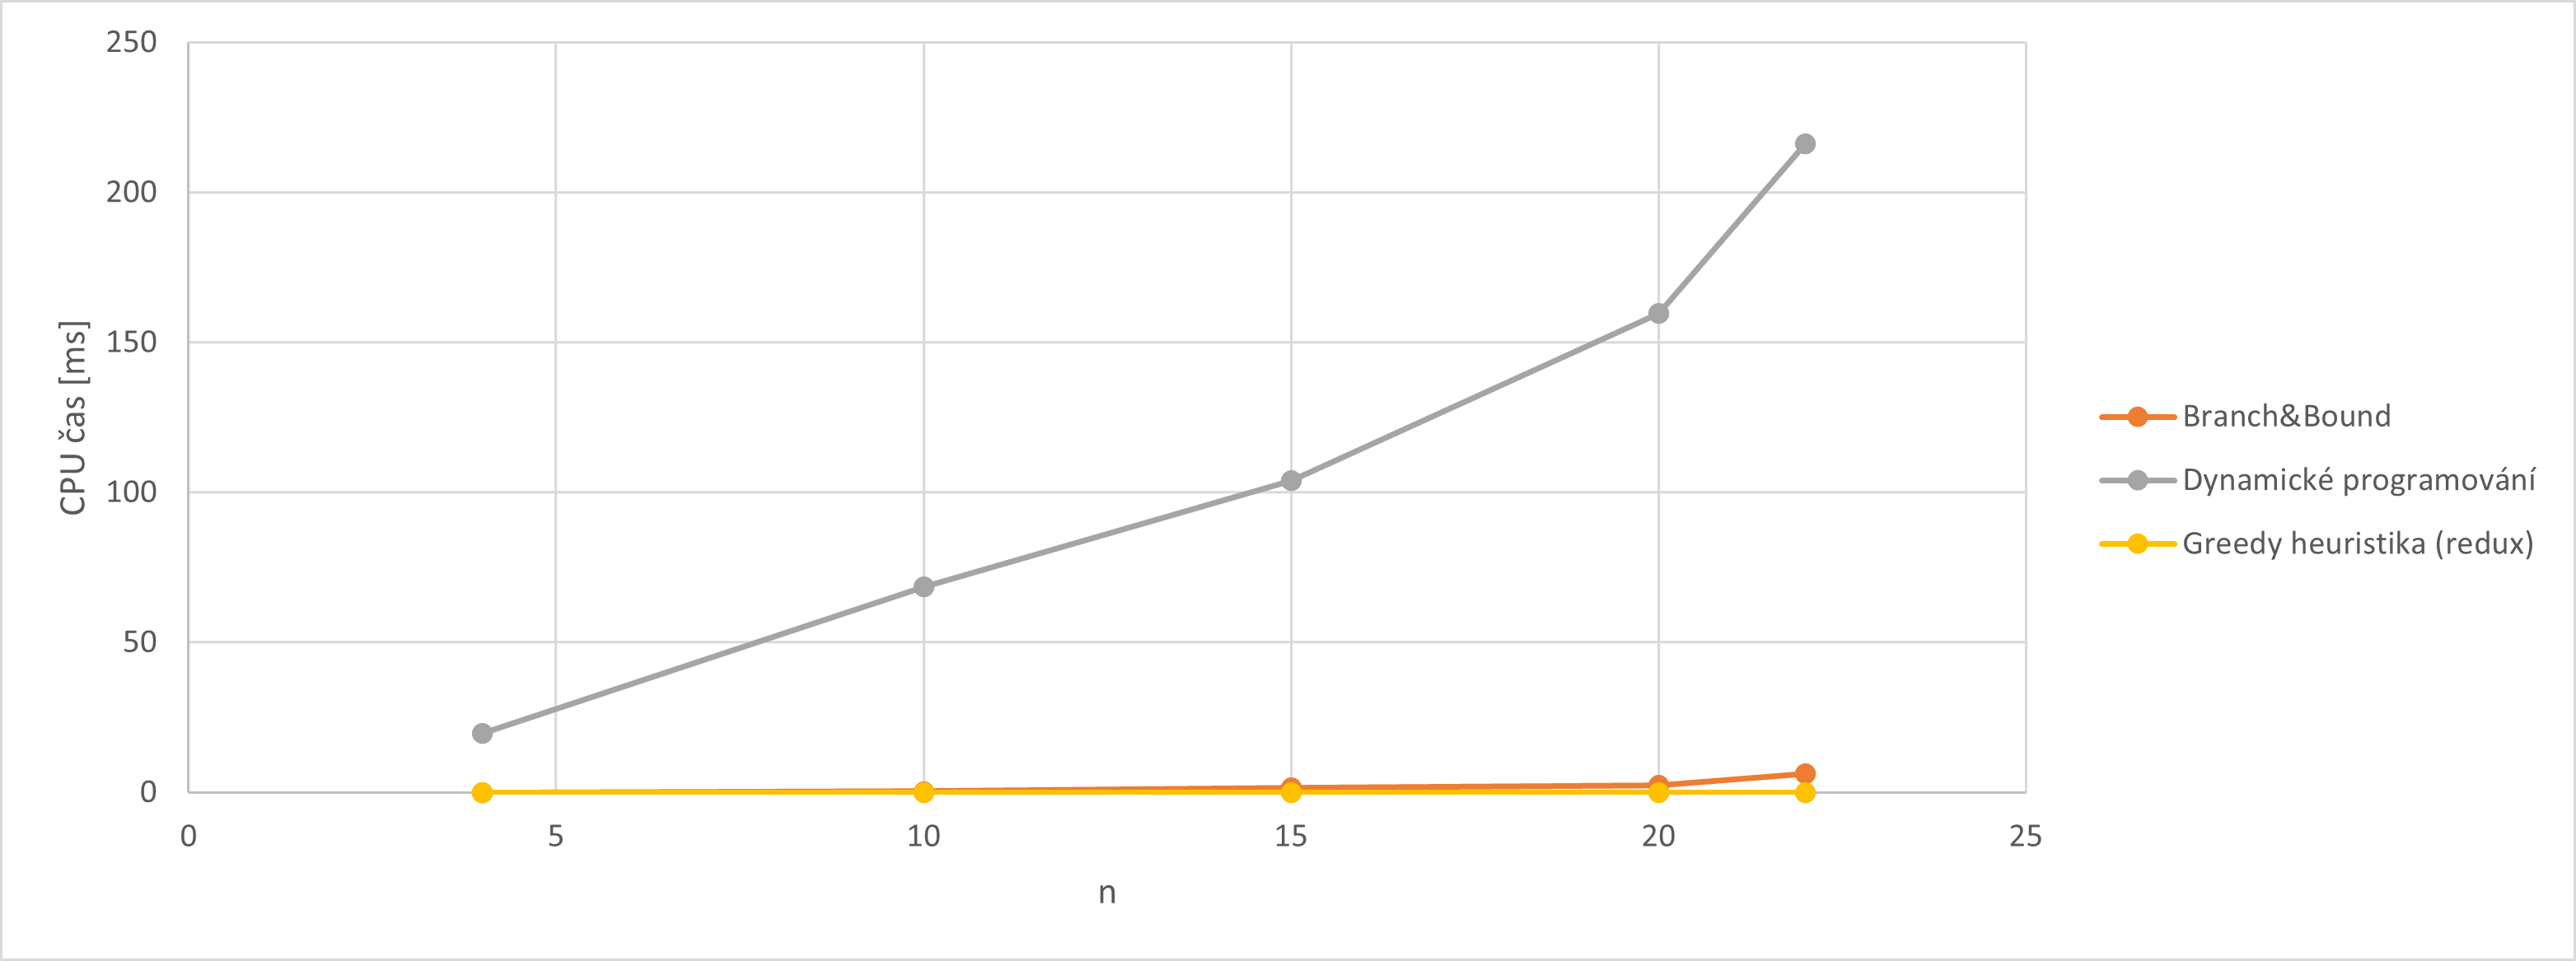
\includegraphics[width=1\textwidth, keepaspectratio]{graphs/ZKW/times/zkw_cpu_time_avg_without_brute_force.png}
    \caption{Závislost průměrného CPU času (bez BruteForce) na n (sada ZKW)}
    \label{fig:zkw_cpu_time_avg_without_brute_force}
\end{figure}

\begin{figure}[ht]\centering
    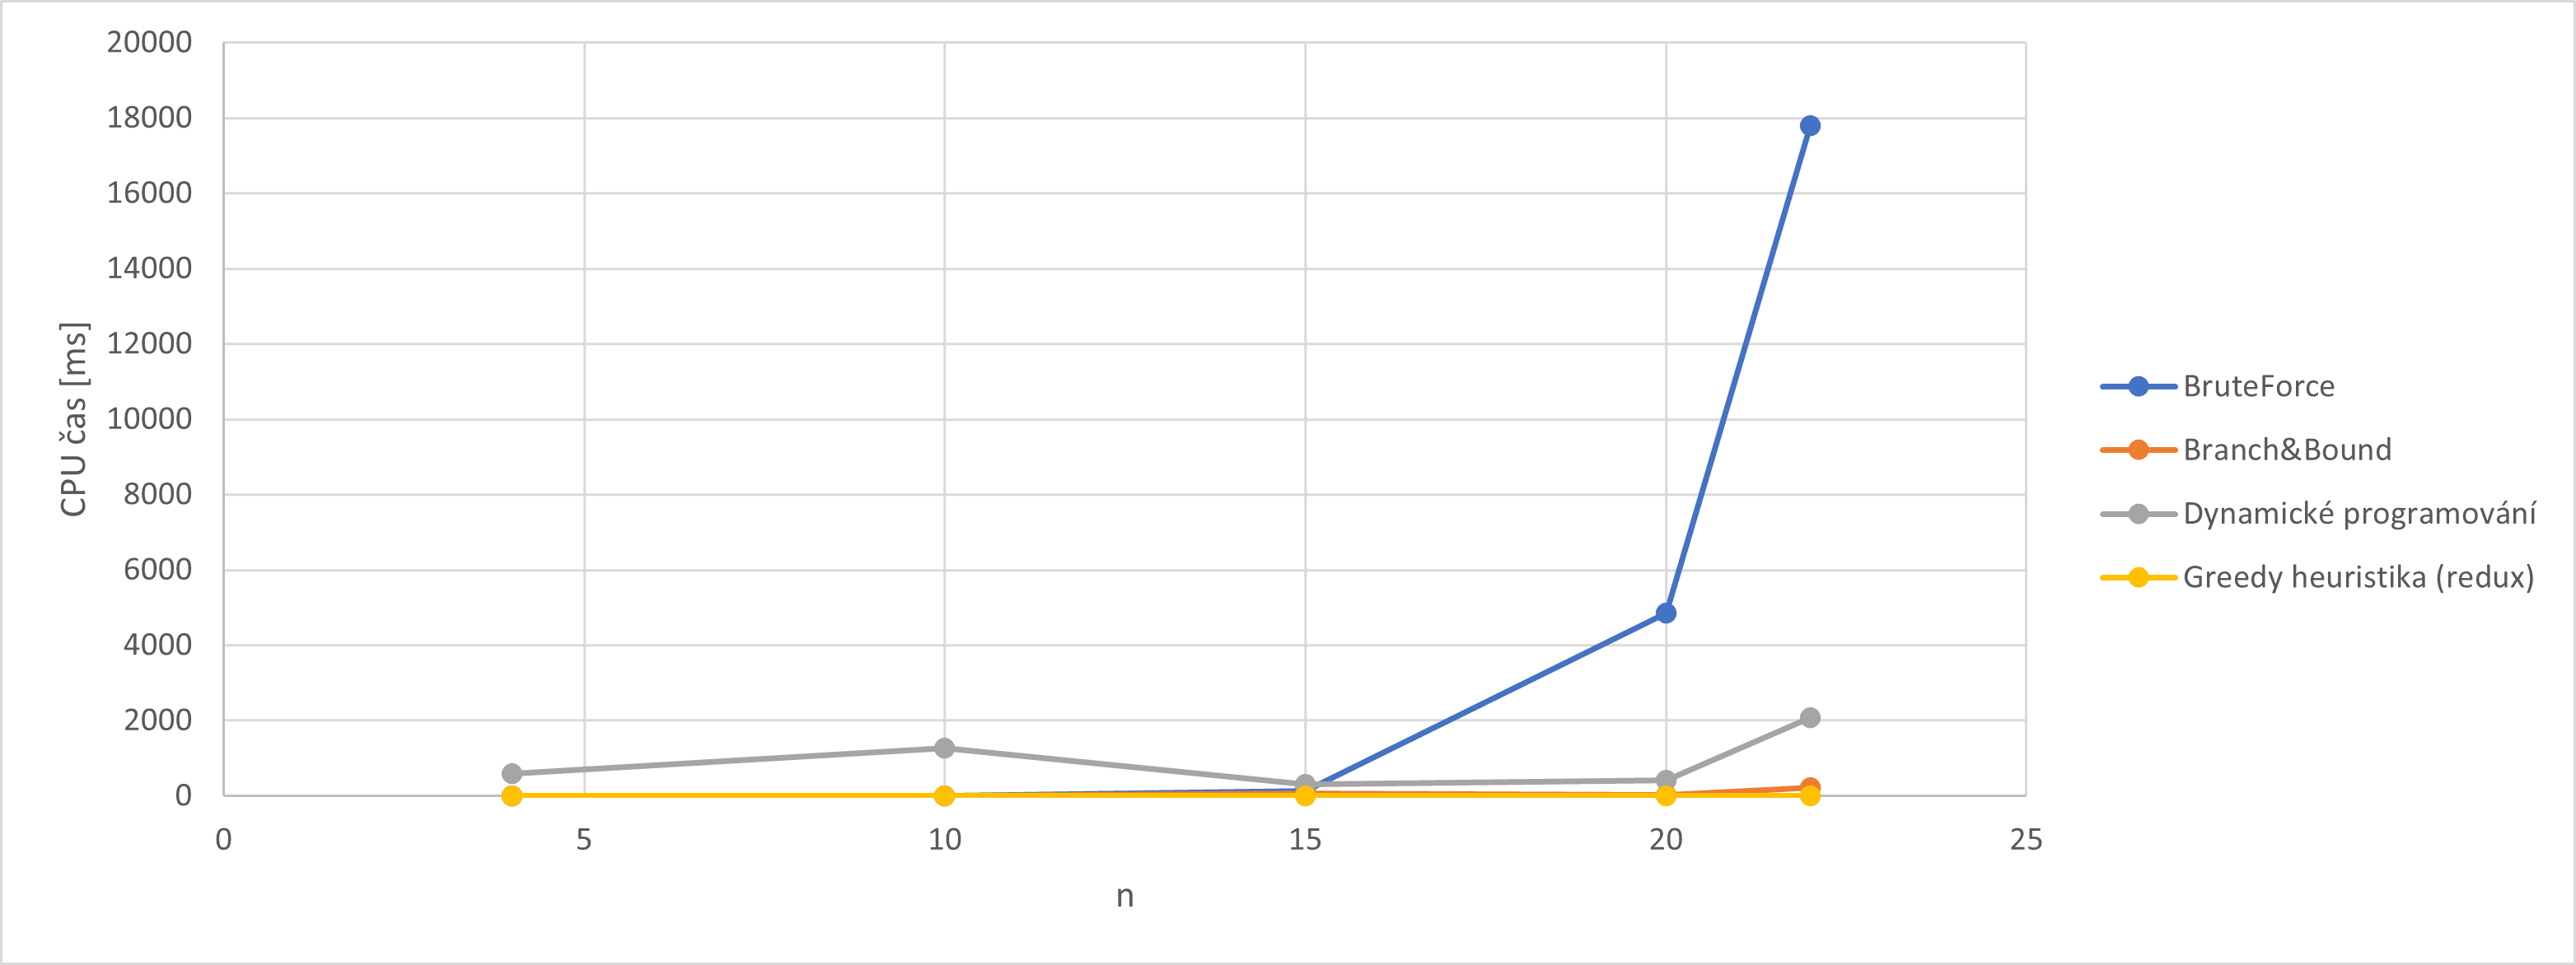
\includegraphics[width=1\textwidth, keepaspectratio]{graphs/ZKW/times/zkw_cpu_time_max.png}
    \caption{Závislost maximálního CPU času na n (sada ZKW)}
    \label{fig:zkw_cpu_time_max}
\end{figure}

\begin{figure}[ht]\centering
    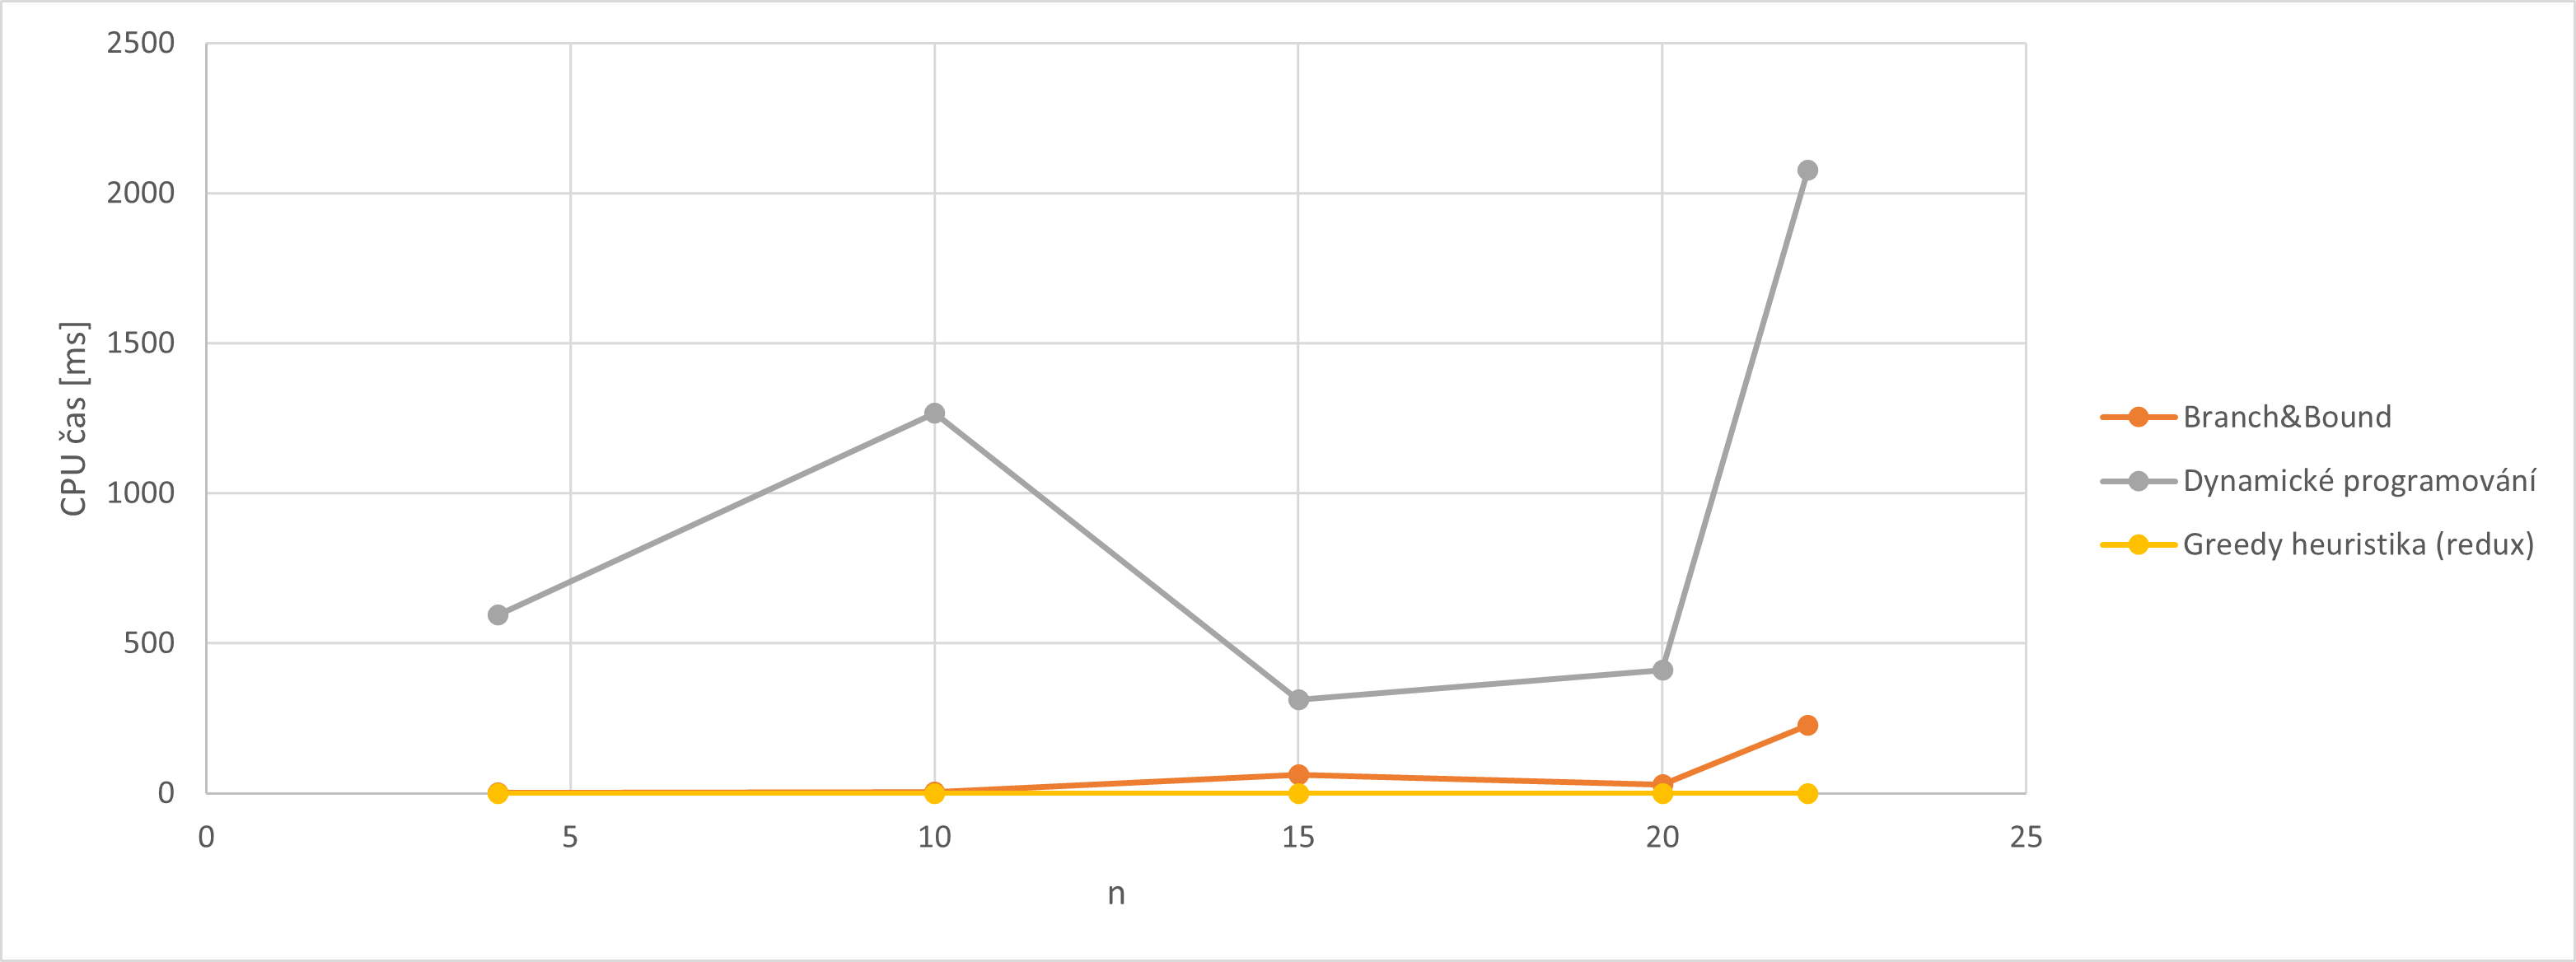
\includegraphics[width=1\textwidth, keepaspectratio]{graphs/ZKW/times/zkw_cpu_time_max_without_brute_force.png}
    \caption{Závislost maximálního CPU času (bez BruteForce) na n (sada ZKW)}
    \label{fig:zkw_cpu_time_max_without_brute_force}
\end{figure}

\subsubsection{Relativní chyby greedy heuristik}

Naměřené údaje jsou k dispozici v tabulce \ref{tab:zkw_greedy_error}. Závislosti jsou vizualizovány v grafech \ref{fig:zkw_greedy_avg} a \ref{fig:zkw_greedy_max}.

\begin{table}
    \begin{center}
         \begin{tabular}{|c | c | c | c | c|} 
         \hline
         n & Greedy & Greedy max & Greedy redux & Greedy redux max \\ [0.1ex] 
         \hline\hline
        4 & 34,446 & 99,422 & 0,001 & 0,001 \\
        \hline
        10 & 23,776 & 98,090 & 0,152 & 9,303 \\
        \hline
        15 & 19,691 & 91,190 & 0,153 & 7,515 \\
        \hline
        20 & 19,641 & 87,070 & 0,266 & 10,455 \\
        \hline
        22 & 23,562 & 98,686 & 0,260 & 8,831 \\
        \hline
        \end{tabular}
        \caption{Relativní chyby greedy heuristik (sada ZKW)} \label{tab:zkw_greedy_error}
    \end{center}
\end{table}

\begin{figure}[ht]\centering
    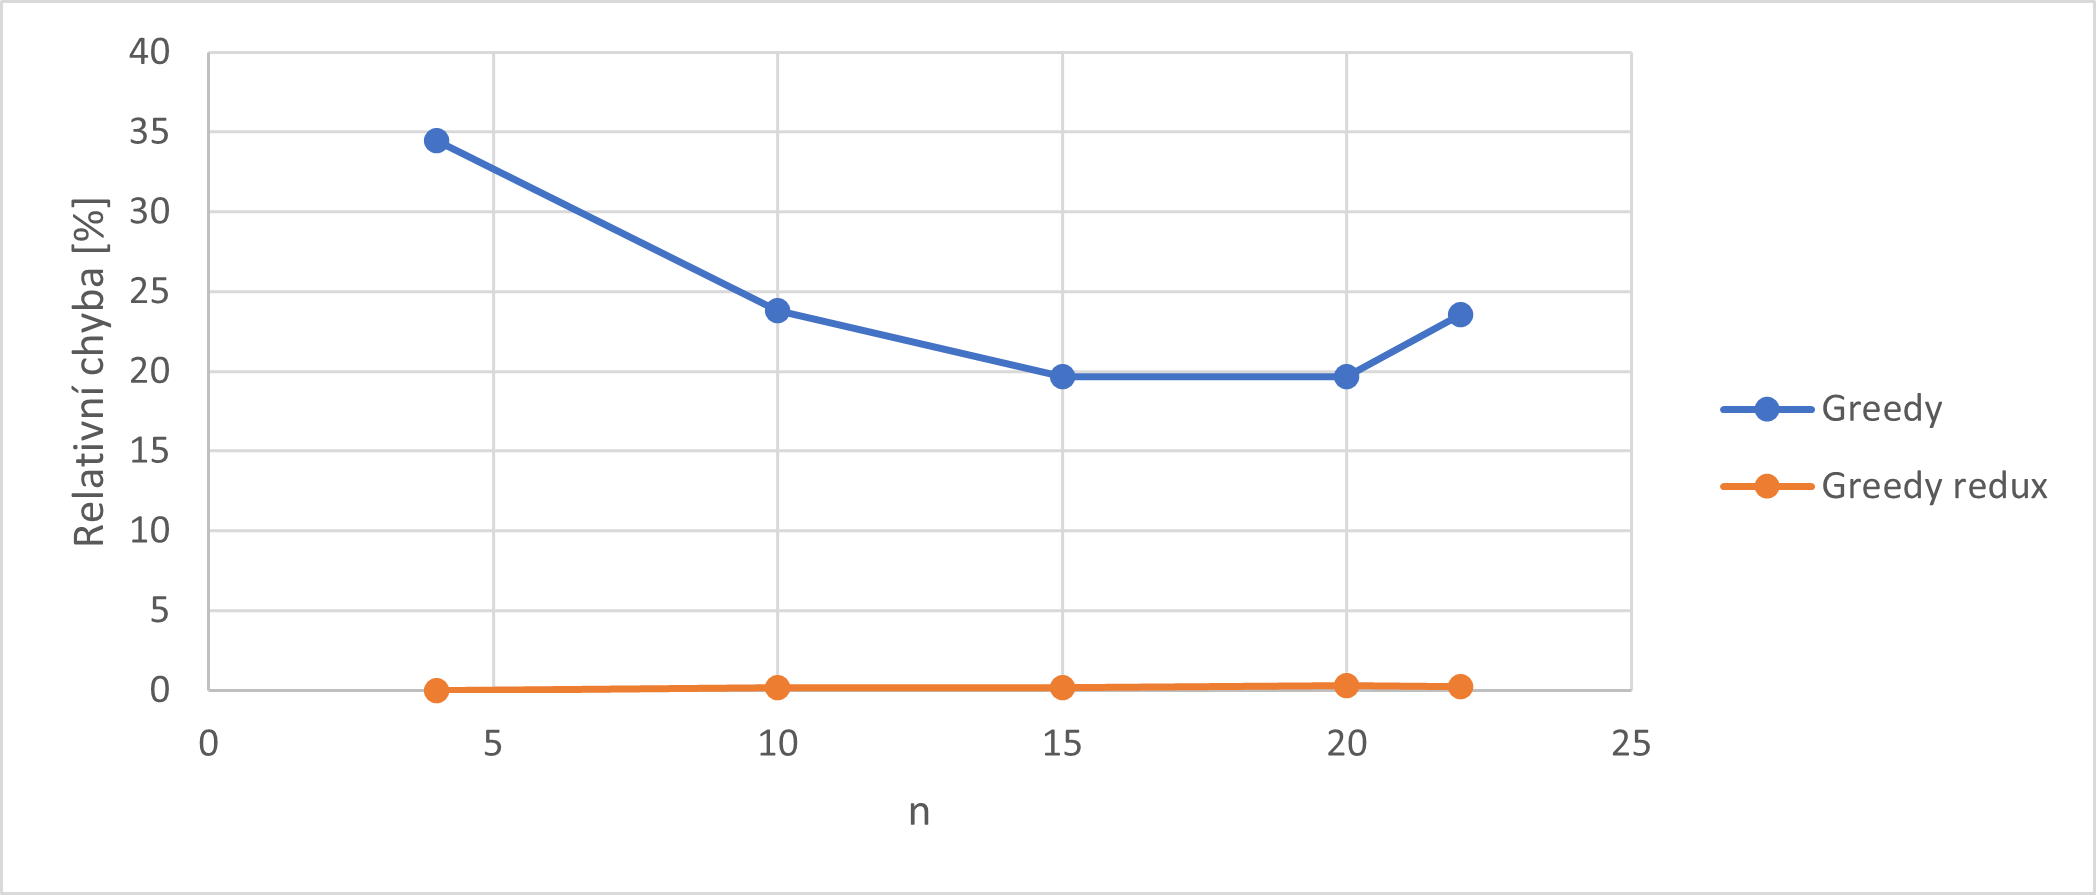
\includegraphics[width=1\textwidth, keepaspectratio]{graphs/ZKW/heuristics/zkw_greedy_avg.png}
    \caption{Průměrná relativní chyba heuristik (sada ZKW)}
    \label{fig:zkw_greedy_avg}
\end{figure}

\begin{figure}[ht]\centering
    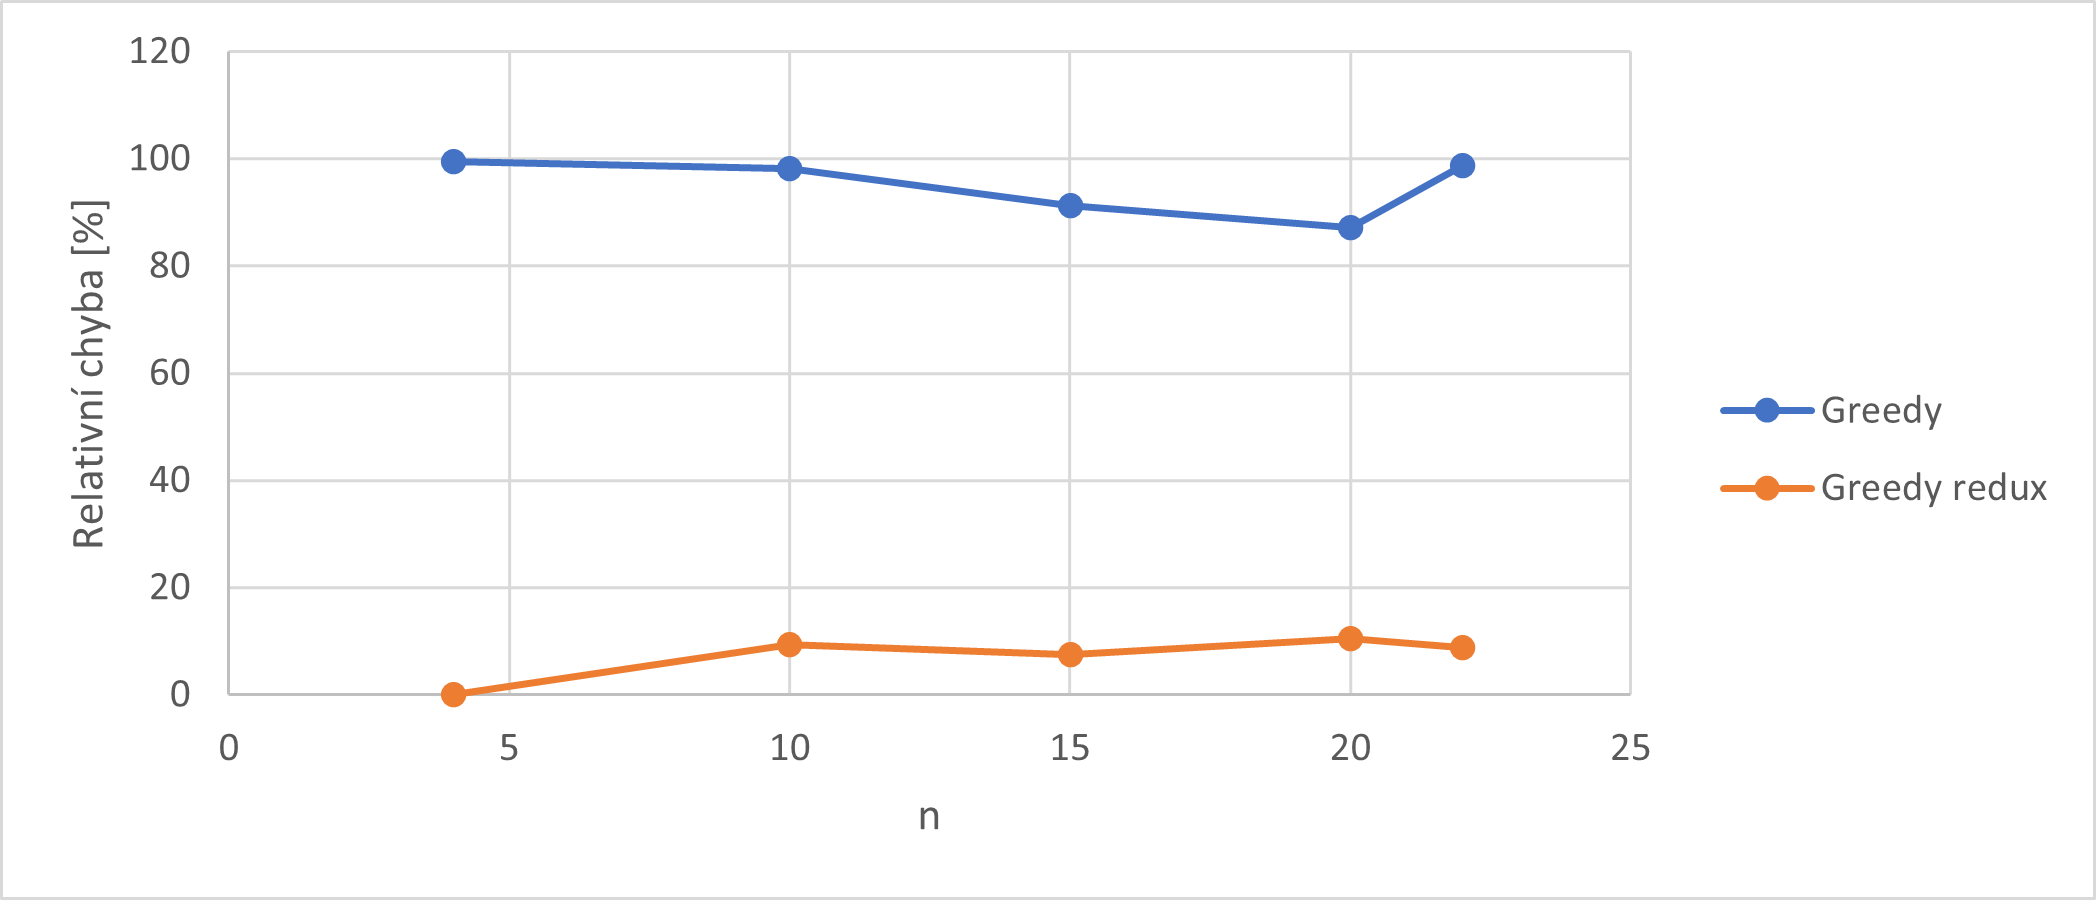
\includegraphics[width=1\textwidth, keepaspectratio]{graphs/ZKW/heuristics/zkw_greedy_max.png}
    \caption{Maximální relativní chyba heuristik (sada ZKW)}
    \label{fig:zkw_greedy_max}
\end{figure}

\subsubsection{CPU čas a chyby algoritmu FPTAS}

Naměřené hodnoty CPU času jsou k dispozici v tabulce \ref{tab:zkw_fptas_eps_times}. Závislosti CPU času jsou vizualizovány v grafech \ref{fig:zkw_fptas_eps_time_avg} a \ref{fig:zkw_fptas_eps_time_max}.
Naměřené hodnoty chyb jsou k dispozici v tabulce \ref{tab:zkw_fptas_eps_error}. Závislosti reálné chyby FPTAS algoritmu jsou vizualizovány v grafu \ref{fig:zkw_fptas_eps_error}. Srovnání reálné a maximální předpokládané chyby algoritmu FPTAS je k dispozici v grafu~\ref{fig:zkw_fptas_eps_error_comparison}.

\begin{table}
    \begin{center}
         \begin{tabular}{|c | c | c | c | c | c | c|} 
         \hline
         $\epsilon$ & n=15 & n=15 (max) & n=20 & n=20 (max) & n=22 & n=22 (max) \\ [0.1ex] 
         \hline\hline
        0,1 & 2,139 & 8 & 3,147 & 11 & 3,726 & 16 \\
        \hline
        0,2 & 1,006 & 3 & 1,615 & 6 & 1,840 & 8 \\
        \hline
        0,3 & 0,617 & 2 & 1,004 & 4 & 1,194 & 5 \\
        \hline
        0,4 & 0,500 & 2 & 0,771 & 3 & 0,903 & 4 \\
        \hline
        0,5 & 0,431 & 1 & 0,623 & 2 & 0,747 & 3 \\
        \hline
        0,6 & 0,383 & 1 & 0,476 & 2 & 0,608 & 3 \\
        \hline
        0,7 & 0,323 & 1 & 0,381 & 2 & 0,481 & 2 \\
        \hline
        0,8 & 0,240 & 1 & 0,312 & 1 & 0,409 & 2 \\
        \hline
        0,9 & 0,128 & 1 & 0,281 & 1 & 0,342 & 2 \\
        \hline
        \end{tabular}
        \caption{CPU časy algoritmus FPTAS v závilosti na $\epsilon$ (sada ZKC)} \label{tab:zkw_fptas_eps_times}
    \end{center}
\end{table}

\begin{figure}[ht]\centering
    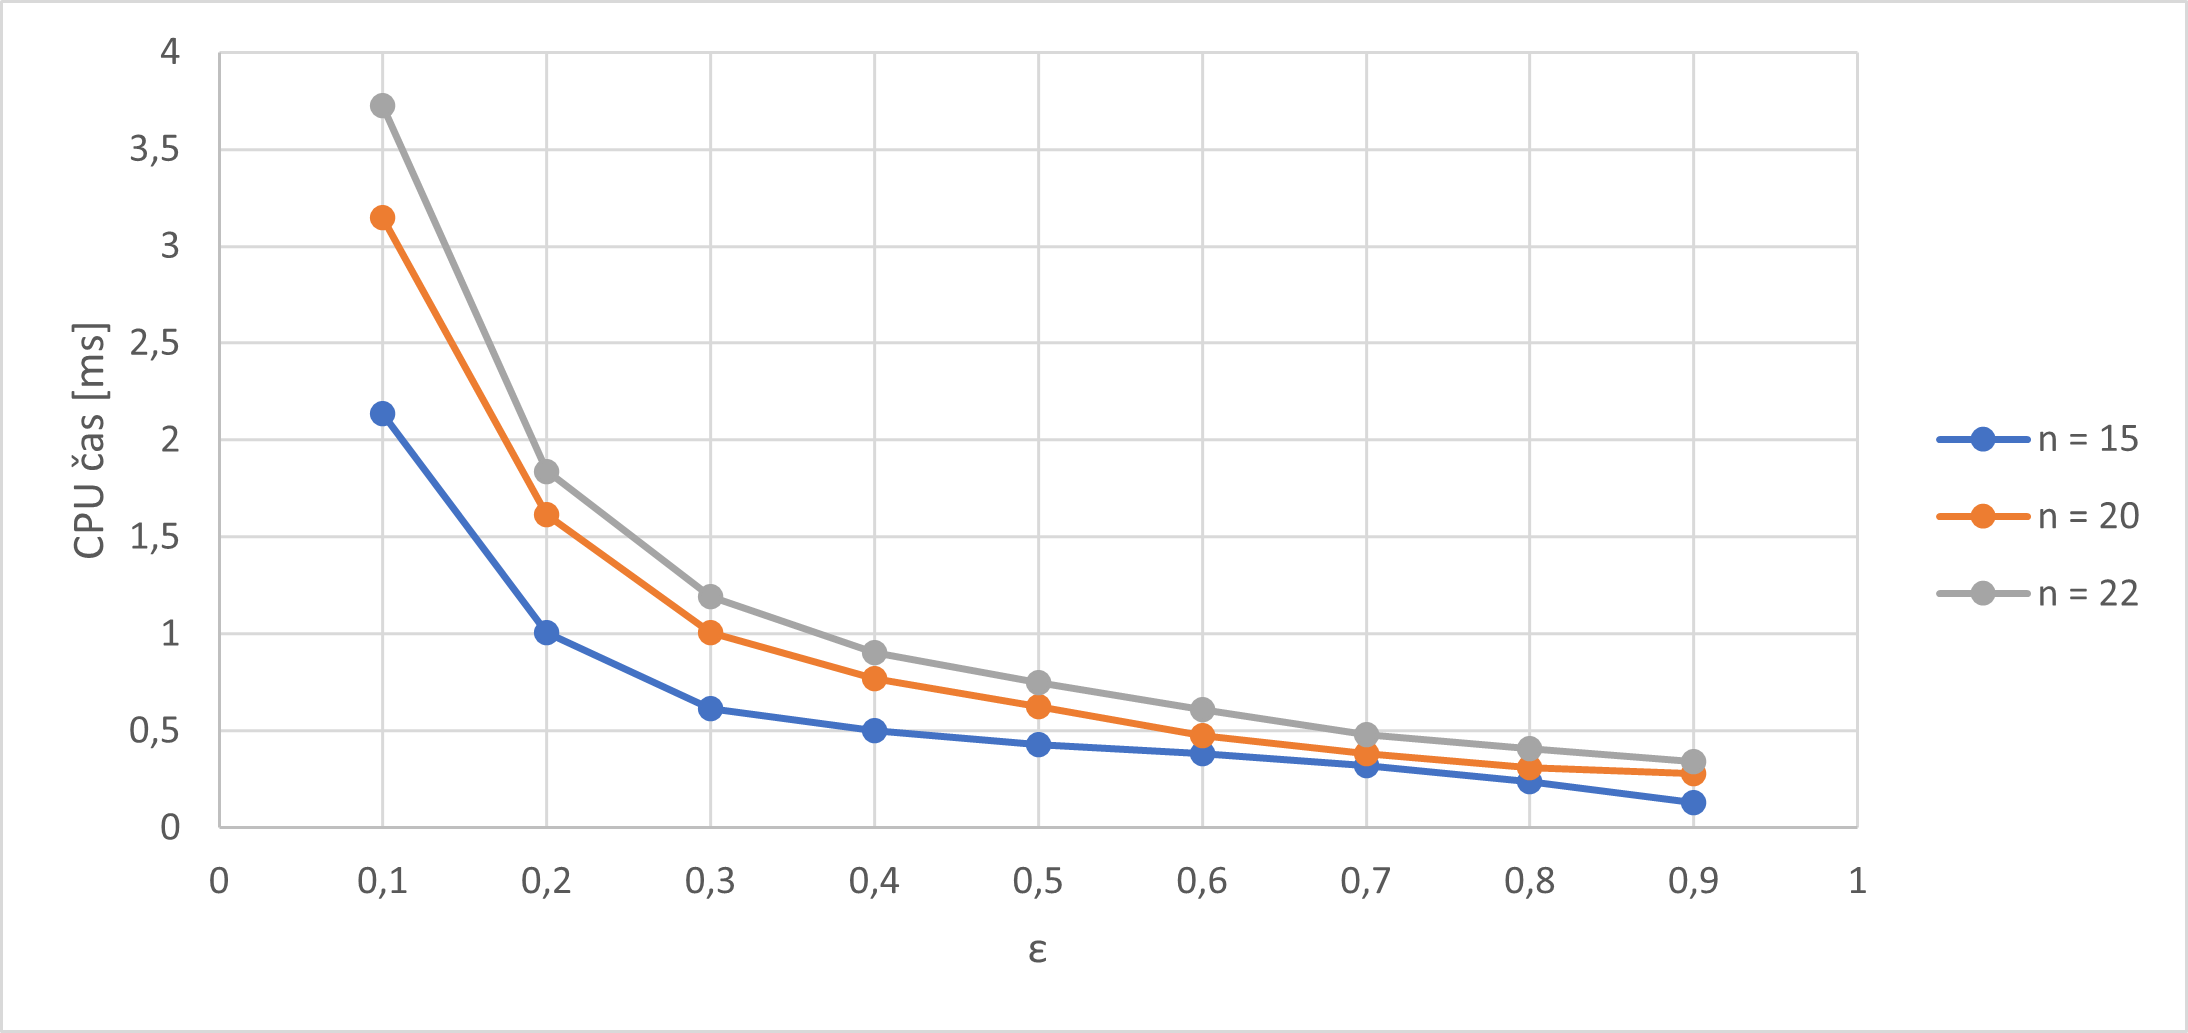
\includegraphics[width=1\textwidth, keepaspectratio]{graphs/ZKW/fptas/zkw_fptas_time_eps_avg.png}
    \caption{Závislost průměrného CPU času FPTAS na $\epsilon$ (sada ZKW)}
    \label{fig:zkw_fptas_eps_time_avg}
\end{figure}

\begin{figure}[ht]\centering
    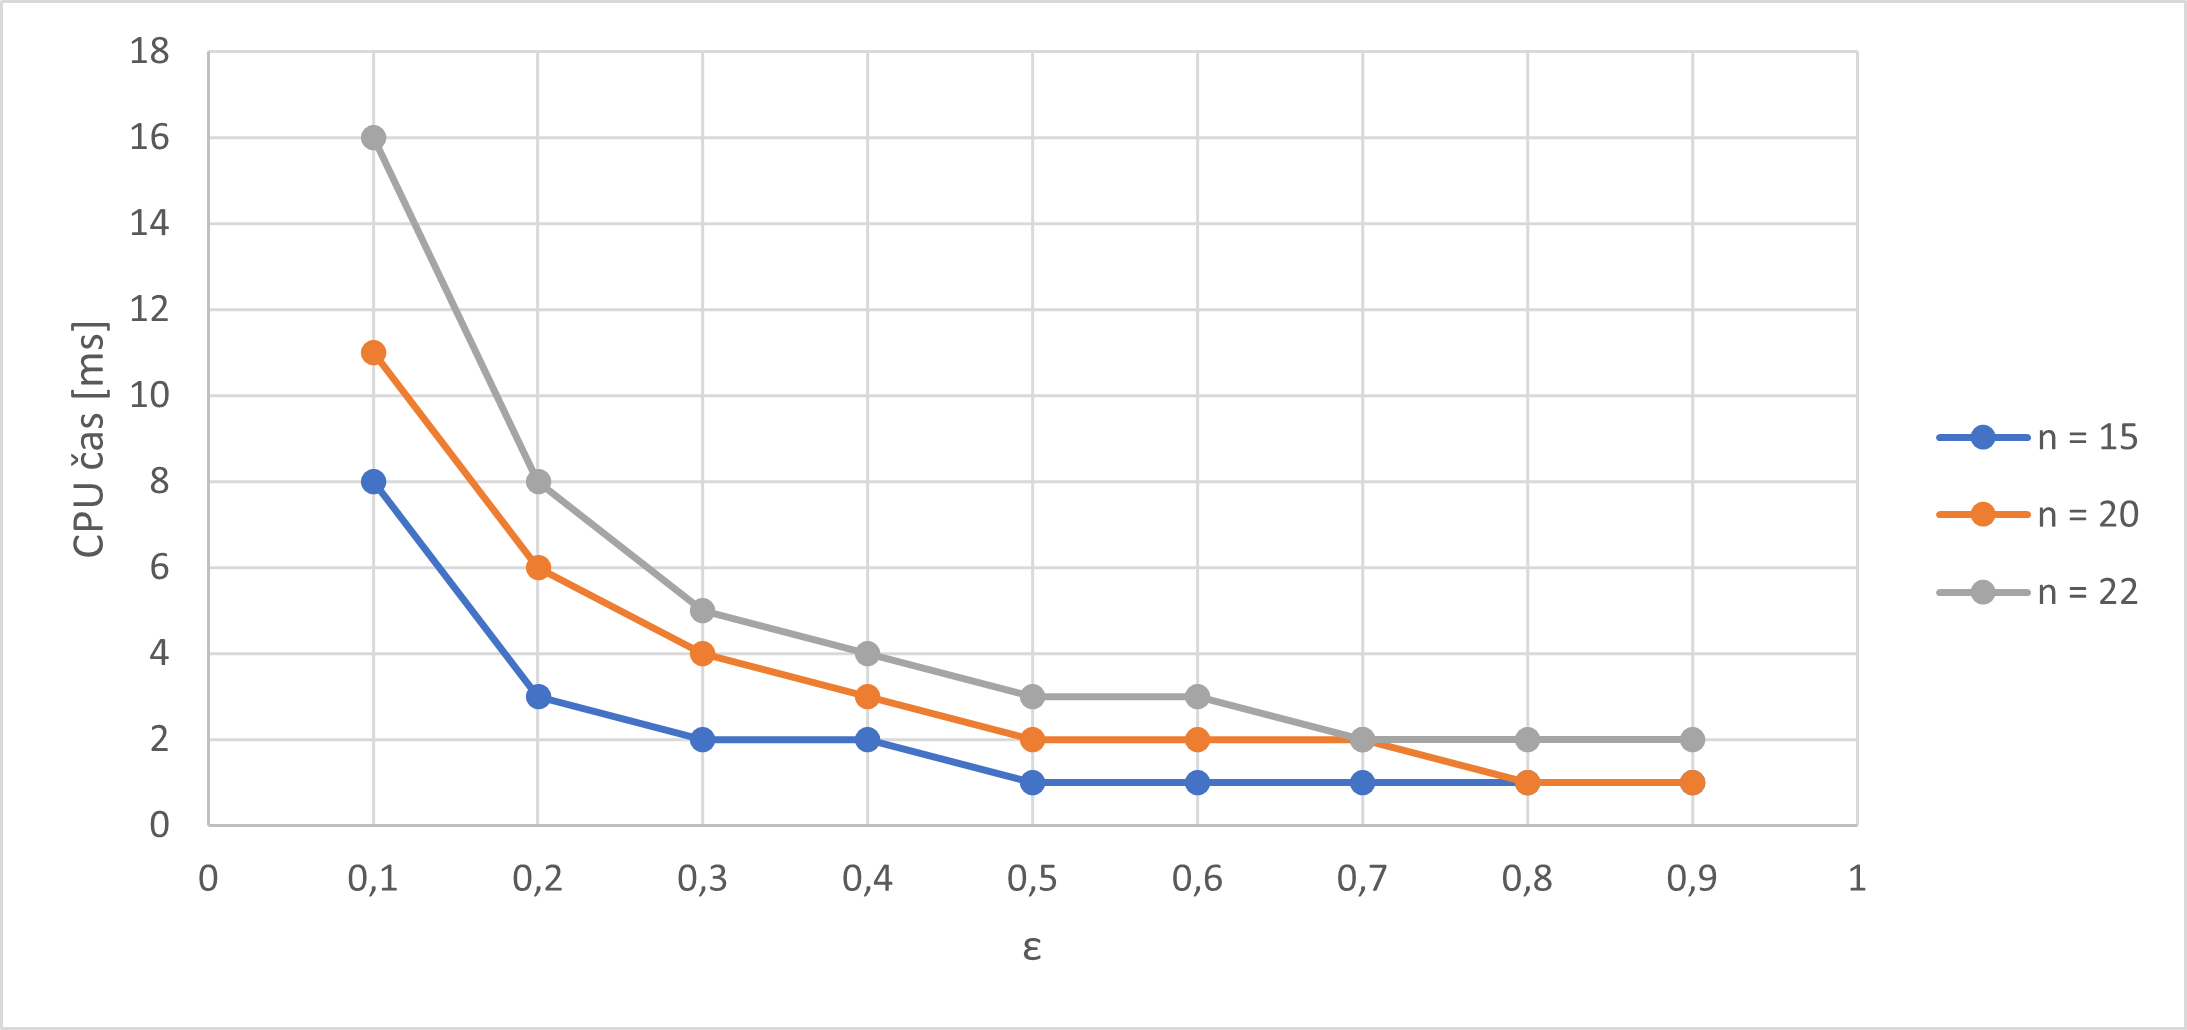
\includegraphics[width=1\textwidth, keepaspectratio]{graphs/ZKW/fptas/zkw_fptas_time_eps_max.png}
    \caption{Závislost maximálního CPU času FPTAS na $\epsilon$ (sada ZKW)}
    \label{fig:zkw_fptas_eps_time_max}
\end{figure}

\begin{table}
    \begin{center}
         \begin{tabular}{|c | c | c | c | c | c | c|} 
         \hline
         $\epsilon$ & n=15 & n=15 (předpoklad) & n=20 & n=20 (předpoklad) & n=22 & n=22 (předpoklad) \\ [0.1ex] 
         \hline\hline
        0,1 & 65 & 664,800 & 109 & 414,500 & 22 & 672,400 \\
        \hline
        0,2 & 507 & 2799,800 & 128 & 1450 & 63 & 830,800 \\
        \hline
        0,3 & 731 & 3421,800 & 205 & 629,100 & 183 & 3325,200 \\
        \hline
        0,4 & 731 & 4562,400 & 173 & 1861,200 & 201 & 1389,600 \\
        \hline
        0,5 & 731 & 5703 & 268 & 3361 & 183 & 5542 \\
        \hline
        0,6 & 731 & 6843,600 & 268 & 4033,200 & 201 & 2084,400 \\
        \hline
        0,7 & 1146 & 7564,900 & 724 & 1723,400 & 350 & 2834,300 \\
        \hline
        0,8 & 803 & 6473,600 & 804 & 6521,600 & 701 & 3239,200 \\
        \hline
        0,9 & 1146 & 9726,300 & 764 & 8974,800 & 1140 & 11349 \\
        \hline
        \end{tabular}
        \caption{Maximální reálné a předpokládané chyby algoritmu FPTAS v závislosti na $\epsilon$ (sada ZKW)} \label{tab:zkw_fptas_eps_error}
    \end{center}
\end{table}

\begin{figure}[ht]\centering
    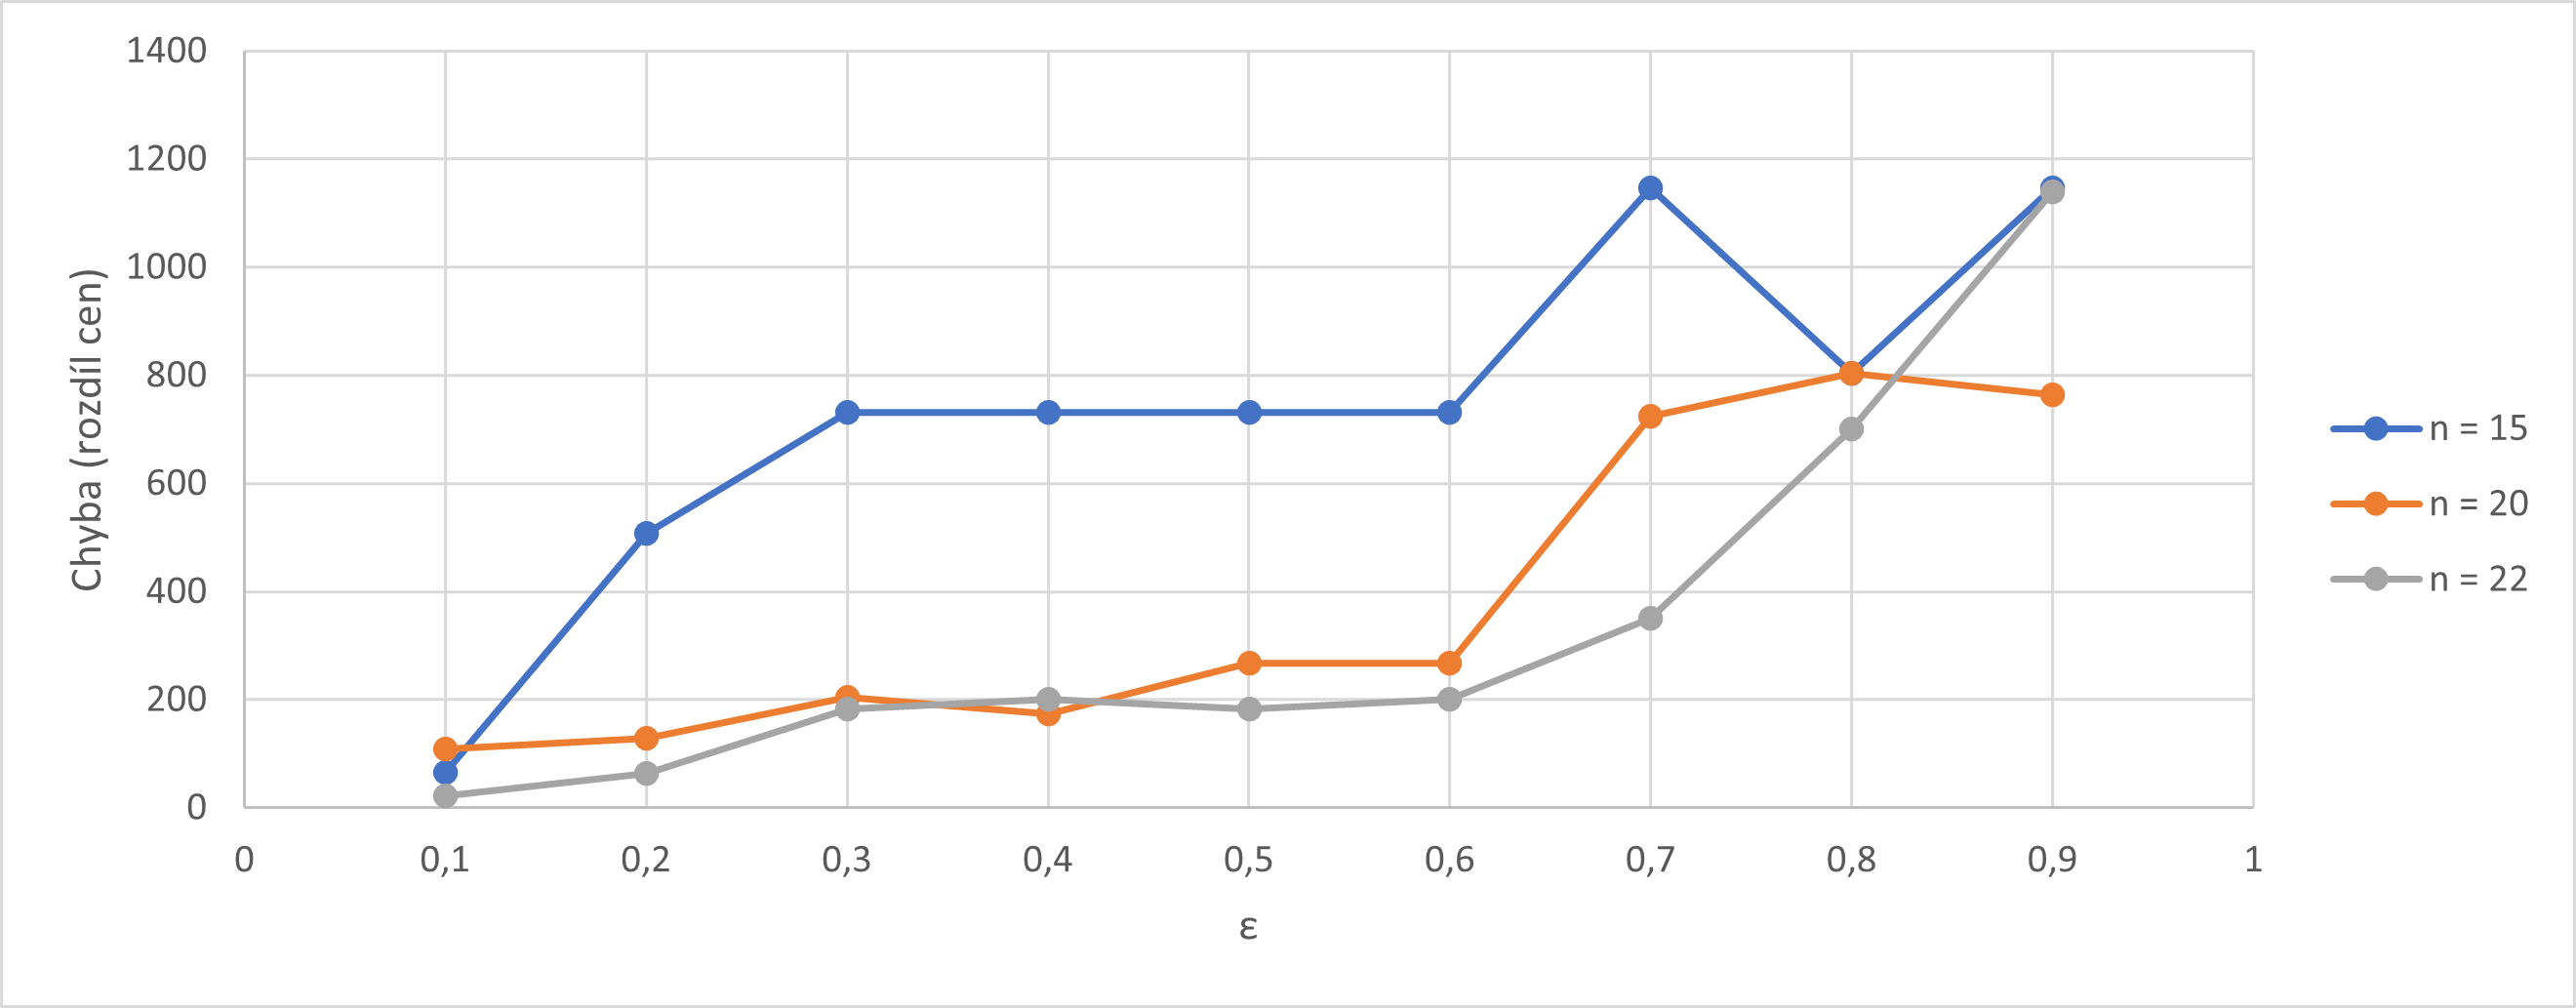
\includegraphics[width=1\textwidth, keepaspectratio]{graphs/ZKW/fptas/zkw_fptas_eps_error.png}
    \caption{Závislost maximální reálné chyby FPTAS na $\epsilon$ (sada ZKW)}
    \label{fig:zkw_fptas_eps_error}
\end{figure}

\begin{figure}[ht]\centering
    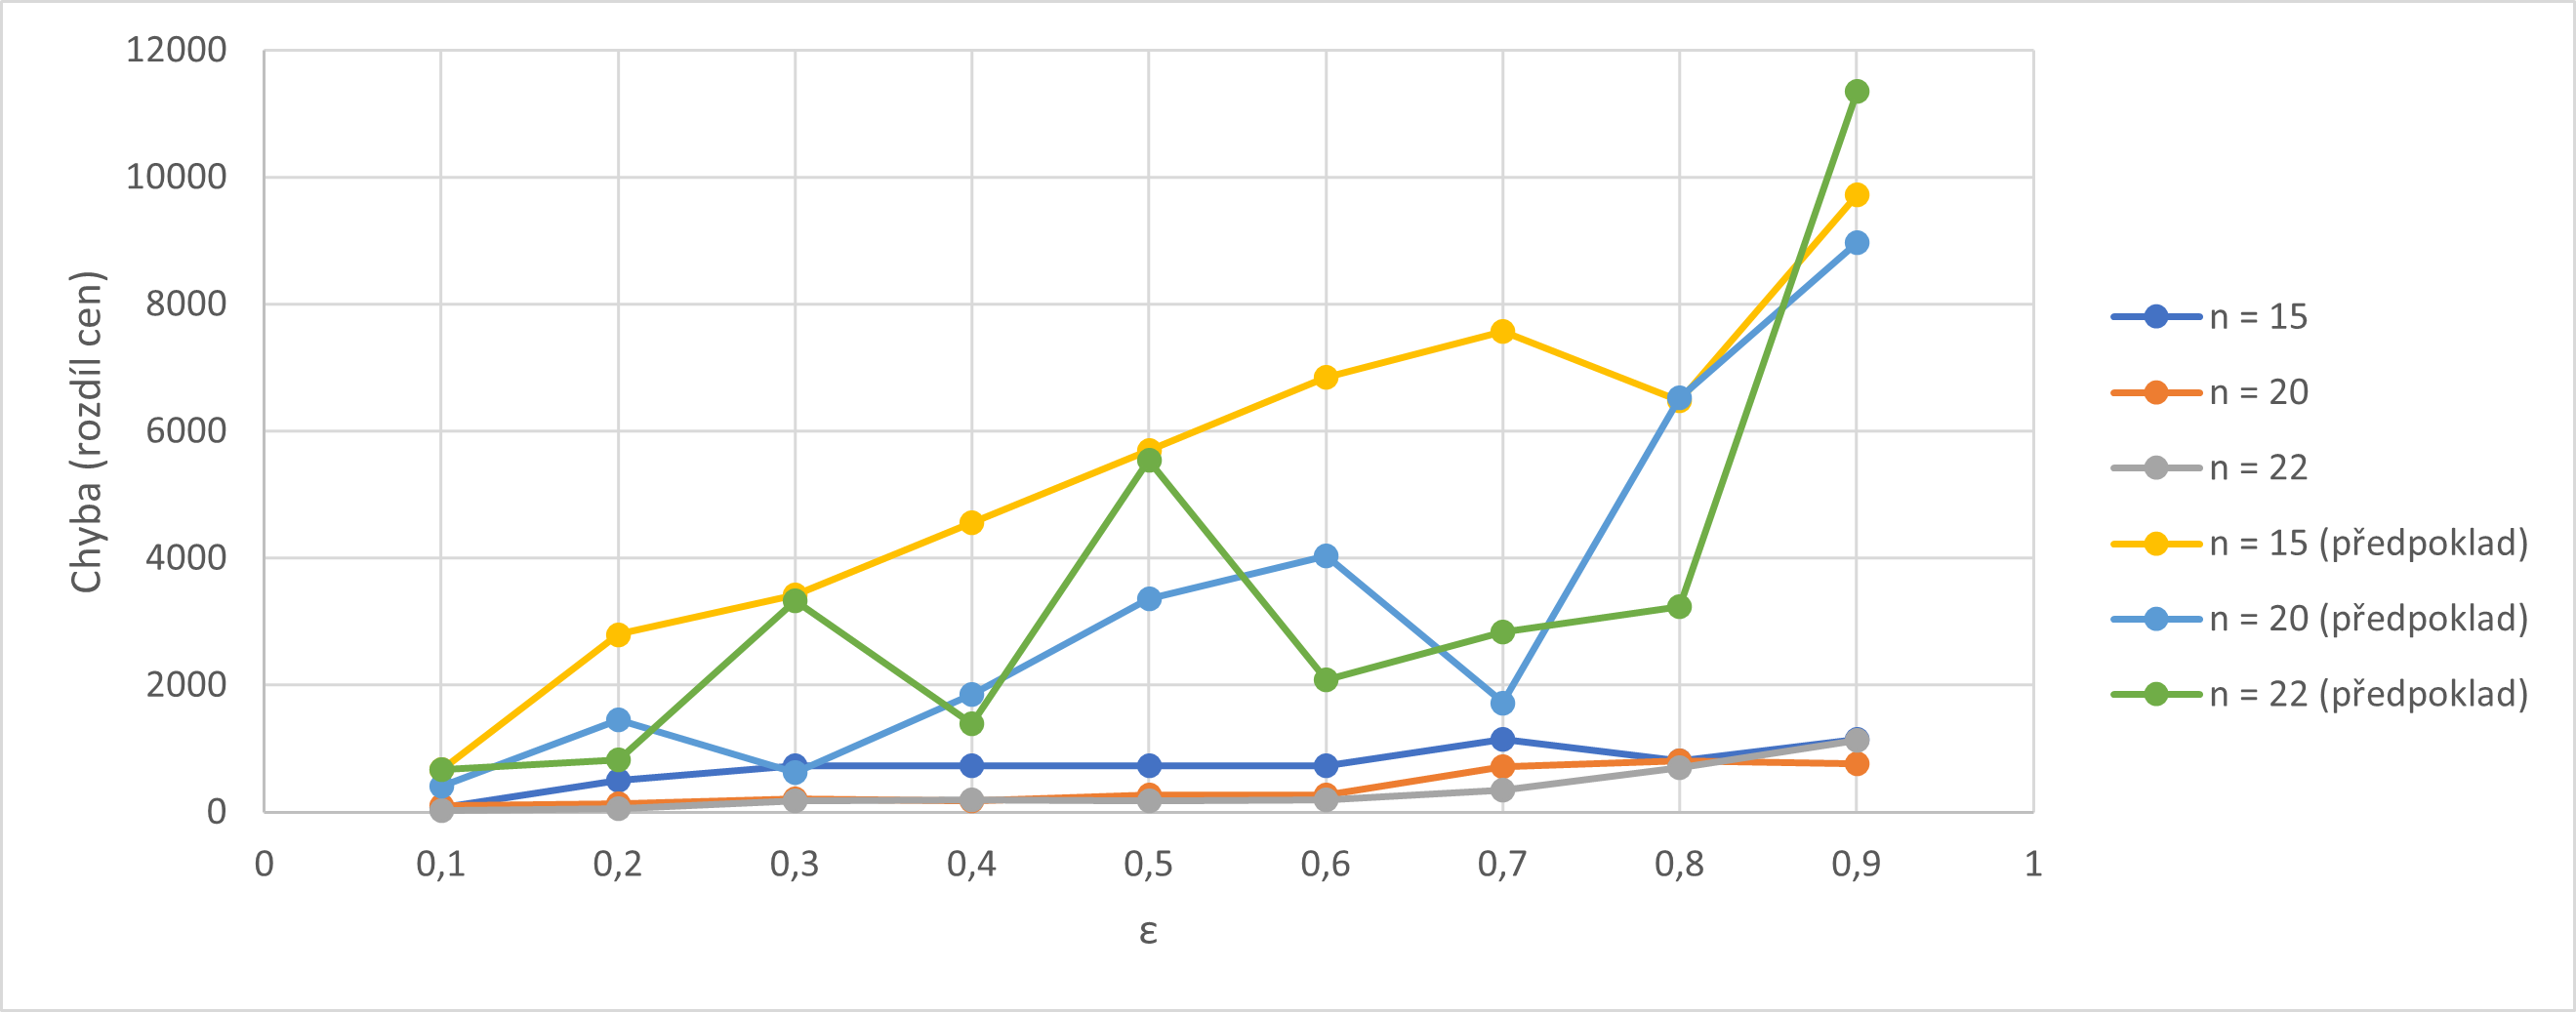
\includegraphics[width=1\textwidth, keepaspectratio]{graphs/ZKW/fptas/zkw_fptas_eps_error_comparison.png}
    \caption{Srovnání maximální reálné chyby FPTAS s předpokládanou horní mezí v závislosti na $\epsilon$ (sada ZKW)}
    \label{fig:zkw_fptas_eps_error_comparison}
\end{figure}

\section{Zhodnocení naměřených výsledků}

Z naměřených dat můžeme pozorovat, že CPU čas metod BruteForce i B\&B má v závislosti na velikosti instance exponenciální tendenci růstu na všech datových sadách. Růst CPU času metody BruteForce je ve všech případech výrazně rychlejší. Nejpomaleji roste CPU čas metody B\&B na datové sadě ZKW. Průměrný CPU čas DP na sadách NK a ZKW a maximální CPU čas DP na ZKW je vyšší než v případě B\&B. Greedy herustika ve srovnání s ostatními metodami roste velmi pomalu.

Můžeme pozorovat, že relativní chyba redux heuristiky je shora omezena relativní chybou základní greedy heuristiky. Na sadách NK a ZKC lze pozorovat, že relativní chyba má s rostoucí velikostí instance tentenci klesat. V případě sady ZKW se chyba základní greedy heuristiky pro instance o velikosti 22 mírně zvýšila. Zároveň lze pozorovat vysokou chybovost základní greedy heuristiky na sadě ZKW. Maximální chyba základní heuristiky překročila hranici 50 \% relativní chyby také při měření maximální rel. chyby nad sadou NK. Redux heuristika dle očekávání tuto hranici při žádném z měření nepřekročila. Nejmenší rozdíl mezi heuristikami lze pozorovat při měření nad sadou ZKC, výrazný rozdíl je pak vidět při měření nad sadou ZKW.

Dále lze pozorovat závislost mezi CPU časem algoritmu FPTAS a maximální povolenou relativní chybou $\epsilon$. S menší povolenou chybou CPU čas roste. Trend růstu přitom připomíná exponenciálu. Nejméně stabilní bylo měření maximální chyby nad sadou ZKC.

Můžeme pozorovat rostoucí reálnou chybu FPTAS algoritmu při zvyšujícím se $\epsilon$. Při srovnání naměřené reálné chyby s předpokládanou maximální chybou jsou naměřené chyby dle očekávání shora omezeny předpokládaným maximem. Nejméně stabilní bylo měření maximální reálné chyby nad sadou ZKW, kde se naměřené hodnoty také nejvíce blížily předpokládanému maximu.

\end{document}
